% $Id$
% \def\QM {{,\kern -0.9 pt ,}}
\setcounter{theorem}{0}
\setcounter{definition}{0}

% ..........................................................................
% --------------------------------------------------------------------------
% ++++++++++++++++++++++++++++++++++++++++++++++++++++++++++++++++++++++++++
%              E l e m e n t a r e  Z a h l e n t h e o r i e
% /~~~~~~~~~~~~~~~~~~~~~~~~~~~~~~~~~~~~~~~~~~~~~~~~~~~~~~~~~~~~~~~~~~~~~~~~~

\newpage
\hypertarget{Chapter_ElementaryNT}{}
\chapter{Introduction to Elementary Number Theory with Examples}
\label{Chapter_ElementaryNT}
(Bernhard Esslinger, July 2001; Updates: Dec. 2001, June 2002, May 2003,
 May 2005, March 2006, June 2007, July 2009) \\

This ``introduction'' is for people with a mathematical interest. There is no
more pre-knowledge necessary than what you learn in the secondary school.\par

We intentionally had ``beginners'' in mind; we did not take the approach
of mathematical textbooks, called ``introduction'', which cannot be
understood at the first reading further than page 5 and which have the real
purpose to deliver all information that special monographs can be read.



% ++++++++++++++++++++++++++++++++++++++++++++++++++++++++++++++++++++++++++
\section{Mathematics and cryptography}
A large proportion of modern, asymmetric cryptography\index{Encryption!asymmetric} is based on mathematical knowledge -- on the properties 
(``laws'') of whole numbers, which are investigated in elementary \index{Number theory!elementary} number 
theory. Here, the word ``elementary'' means that questions raised in number theory are essentially rooted in the set 
of natural and whole numbers.

Further mathematical disciplines currently used in cryptography include
(see \cite[p. 2]{nt:Bauer1995}, \cite[p. 3]{nt:Bauer2000}) :
\begin{itemize}
    \item Group theory\index{Group}
    \item Combination theory
    \item Complexity theory
    \item Ergodic theory
    \item Information theory.
\end{itemize}

Number theory or arithmetic (the emphasis here is more on the aspect of 
performing calculations with numbers) was established 
by Carl Friedrich Gauss\footnote{%
  Carl Friedrich Gauss, German mathematician and astronomer,
  Apr 30, 1777$-$Feb 23, 1855.
}
\index{Gauss, Carl Friedrich} as a special mathematical discipline. Its 
elementary features include the greatest common divisor\footnote{This 
article deals with the gcd (greatest common 
divisor)\index{Gcd} in appendix~\ref{NumberTheory_Appendix_GCD}.}
(gcd), congruence (remainder classes), factorization, the Euler-Fermat theorem
and primitive roots. However, the most important 
aspect is prime numbers and their multiplicative operation.

For a long time, number theory was considered to be the epitome of pure research, the ideal example of research 
in the ivory tower. It delved into ``the mysterious laws of the realm of numbers'', giving rise to philosophical 
considerations as to whether it described elements that exist everywhere in nature or whether it artificially 
constructed elements (numbers, operators and properties).

We now know that patterns from number theory can be found everywhere in nature. 
For example, the ratio of 
%laevorotary and dextrorotary 
rotating counterclockwise and rotating clockwise 
spirals in a sunflower is equal to two consecutive 
Fibonacci\index{Fibonacci} numbers\footnote{%
The sequence of Fibonacci numbers $(a_i)_{i \in \mathbb{N}}$ is defined 
by the ``recursive'' rule $a_1 := a_2 := 1$ and for all numbers  $n=1,2,3,\cdots$ 
we define $a_{n+2} := a_{n+1}+a_n$.  
This historical sequence can be found in many interesting forms in nature 
(for example, see \cite[p. 290 ff]{nt:Graham1994}\index{Graham 1994} or the 
website of \hyperlink{knott}{Ron Knott}\index{Knott, Ron}, which is devoted 
to Fibonacci\index{Fibonacci} numbers). A lot is known about the Fibonacci 
sequence and it is used today as an important tool in mathematics.}, for 
example $21 : 34$.

Also, at the latest when number theory was applied in modern cryptography, it became clear that a discipline that 
had been regarded as purely theoretical for centuries actually had a practical use. Today, experts in this field are 
in great demand on the job market.

Applications in (computer) security now use cryptography because this mathematical discipline is simply better 
and easier to prove than all other ''creative'' substitution procedures that have been developed over the course of 
time and better than all sophisticated physical methods such as those used to print bank notes \cite[p. 4]{nt:Beutelspacher1996}.

This article explains the basics of elementary number theory in a way that you can easily understand. It provides 
numerous examples and very rarely goes into any proofs (these can be found in mathematical textbooks).

The goal is not to exhaustively explain the number theory findings, but 
to show the essential procedures. The volume of the content is so oriented
that the reader can understand and apply the RSA method\index{RSA}.

For this purpose we will use both theory and examples to explain how 
to perform calculations in finite sets and describe how these techniques
are applied in cryptography. Particular attention will be paid to the 
traditional Diffie-Hellman\index{Diffie-Hellman} (DH) and RSA public 
key procedures.\index{RSA}

Additionally I added some qualified statements about the security of the RSA algorithm.



\vskip +40 pt

\begin{center}
\fbox{\parbox{15cm}{{\em Carl Friedrich Gauss\index{Gauss, Carl Friedrich}:}\\
Mathematics is the queen of sciences and number theory is the queen of
mathematics.}}
\end{center}

%\begin{quote}
%{\em Carl Friedrich Gauss:}\\
%Mathematics is the queen of sciences and number theory is the queen of mathematics.
%\end{quote}

% ++++++++++++++++++++++++++++++++++++++++++++++++++++++++++++++++++++++++++
\section{Introduction to number theory} \index{Number theory!introduction}

Number theory arose from interest in positive whole numbers $1, 2, 3, 4, \cdots$, also referred to as the set of natural numbers 
\index{Number!natural} {\em natural numbers} $\mathbb{N}$. These are the first mathematical constructs 
used by human civilization. According to Kronecker\footnote{Leopold
  Kronecker, German mathematician, Dec 7, 1823 $-$ Dec 29, 1891}\index{Kronecker, Leopold}, they are a creation of God. 
In Dedekind's\footnote{Julius Wilhelm Richard Dedekind,
  German mathematician, Oct 6, 1831 $-$ Feb 12, 1916.}\index{Dedekind, Julius} opinion, they are a creation of the human intellect. Dependent upon one's ideology,
this is an unsolvable contradiction or one and the same thing.

In ancient times, no distinction was made between number theory and numerology,
which attributed a mystical significance to specific numbers. In the same way
as astronomy and chemistry gradually detached themselves from astrology and
alchemy during the Renaissance (from the 14th century), number theory also
separated itself from numerology.

Number theory has always been a source of fascination -- for both amateurs and
professional mathematicians. In contrast to other areas of mathematics, many
of the problems and theorems in number theory can be understood by non-experts.
On the other hand, the solutions to these problems or the prove to the theorems
often resisted to the mathematicians for a very long time.
It is therefore one thing to pose good questions but quite another matter to
find the answer. One example of this is what is known as Fermat's Last (or
large) theorem\footnote{One of the things we learn in mathematics at school
   is Pythagoras' theorem, which states the following for a right-angle
   triangle: $a^2 + b^2 = c^2$, where $a$ and $b$ are the lengths of the sides
   containing the right angle and $c$ is the length of the hypotenuse.
   Fermat famously proposed that $a^n + b^n \not= c^n$
   for $a,b,c \in \mathbb{N}$ and whole-number exponents $n > 2$.
   Unfortunately, the letter in which Fermat made the claim did not have
   enough space for him to prove it. The theorem was not proven until over
   300 years later \cite[p. 433-551]{nt:Wiles1994}\index{Wiles, Andrew}. }.

Up until the mid 20th century, number theory was considered to be the purest area of mathematics, an area that 
had no practical use in the real world. This changed with the development of computers and digital 
communication, as number theory was able to provide several unexpected solutions to real-life tasks. At the same 
time, advances in information technology allowed specialists in number theory to make huge progress in 
factorizing large numbers, finding new prime numbers, testing (old) conjectures and solving numerical problems 
that were previously impossible to solve. Modern number theory \index{Number theory!modern} is made up of 
areas such as:
\begin{itemize}
    \item Elementary number theory
    \item Algebraic number theory
    \item Analytic number theory
    \item Geometric number theory
    \item Combinatorial number theory
    \item Numeric number theory
    \item Probability theory.
\end{itemize}

All of the different areas are concerned with questions regarding whole numbers (both positive and negative 
whole numbers plus zero). However, they each have different methods of dealing with them.

This article only deals with the area of elementary number theory.


% --------------------------------------------------------------------------
\newpage
\subsection{Convention}
Unless stated otherwise: 
\begin{itemize}
\item The letters $a, b, c, d, e, k, n, m, p, q$ are used to present whole numbers.
\item The letters $i$ ~\mbox{and} $j$ represent natural numbers. 
\item The letters $p$ always represents a prime number.
\item The sets $\mathbb{N} = \{ 1, 2, 3, \cdots \}$ and $\mathbb{Z} =\{ \cdots, -3, -2, -1, 0, 1, 2, 3, \cdots \}$ 
are the {\em natural} and {\em whole} numbers respectively.
\end{itemize}

% \vskip +40 pt
\newpage

\begin{center}
\fbox{\parbox{15cm}{{\em Joanne\index{Rowling,
Joanne} K. Rowling\footnotemark\:}\newline This isn't 
magic -- it's logic -- a puzzle. A lot of the greatest 
wizards haven't got an ounce of logic.}}
\end{center}

\addtocounter{footnote}{0}\footnotetext{Joanne K. Rowling,~``Harry Potter and the Philosopher's Stone'', Bloomsbury, (c) 
1997, chapter ``Through the trapdoor'', p. 307, by Hermine.}


%\begin{quote}
%{\em Joanne K. Rowling\footnote{Joanne K. Rowling,~``Harry Potter and the Philosopher's Stone'', Carlsen, (c) 
%1997, chapter ``Through the trapdoor'', p. 310.}:}\newline This isn't magic -- it's logic -- a puzzle. A 
%lot of the greatest wizards haven't got an ounce of logic.
%\end{quote}


% ++++++++++++++++++++++++++++++++++++++++++++++++++++++++++++++++++++++++++
\section{Prime numbers and the first fundamental theorem of elementary number theory}
\index{Number theory!elementary} Many of the problems in elementary number theory are concerned with prime 
numbers.

Every whole number has divisors or factors. The number 1 has just one -- itself, whereas the number 12 has the 
six factors 1, 2, 3, 4, 6 and 12\footnote{Due to the fact that 12 has so many factors, this number -- and multiples 
of this number -- is often found in everyday life: the 12-hour scale on clocks, the 60 minutes in an hour, the 
360-degree scale for measuring angles, etc. If we divide these scales into segments, the segments often turn out to be whole numbers. 
These are easier to use in mental arithmetic than fractions.}. Many numbers are only divisible by themselves and 
by 1. When it comes to multiplication, these can be regarded as the ``atoms'' in the realm of numbers.

\begin{definition}\label{def-zth-prime} \index{Prime number}
{\bf Prime numbers} are natural numbers greater than 1 that can only be divided by 1 and themselves.
\end{definition}

By definition, $1$ is not a prime number.

If we write down the prime numbers in ascending order (prime number sequence), then we get:
$$2,~ 3,~ 5,~ 7,~11,~ 13,~ 17,~ 19,~ 23,~ 29,~ 31,~ 37,~ 41,~ 43,~ 47,~ 53,~ 59,~ 61,~ 67,~ 71,
~73,~ 79,~ 83,~ 89,~ 97, \cdots.$$

The first $100$ numbers include precisely $25$ prime numbers. After this, the percentage of primes decreases, 
but never reaches zero.

We come across whole numbers that are prime fairly often. In the last decade only, three years were prime: 
$1993, 1997$ and $1999$. If they were rare, cryptography would not be able to work with them to the extent it 
does.

Prime numbers can be factorized in a unique (``{\em trivial}'') way:
\begin{eqnarray*}
5 & = & 1 * 5 \nonumber \\
17 & =  & 1 * 17 \nonumber \\
1013 &  = & 1 * 1013 \nonumber \\
1,296,409 & = & 1 * 1,296,409. \nonumber
\end{eqnarray*}

\begin{definition}\label{def-zth-composite} \index{Number!composite}
Natural numbers greater than $1$ that are not prime are called {\bf composite numbers}. These have at least two 
factors other than $1$.
\end{definition}


Examples of the decomposition of such numbers into prime 
factors\index{Prime factor!decomposition}:
\begin{eqnarray*}
4 & = & 2*2  \nonumber \\
6 & = & 2*3  \nonumber \\
91 & = & 7*13  \nonumber \\
161 & = & 7*23  \nonumber \\
767 & = & 13*59  \nonumber \\
1029 & = & 3 * 7^3  \nonumber \\
5324 & = & 22 * 11^3.  \nonumber 
\end{eqnarray*}

\begin{theorem}\label{thm-zth-cnum}
Each composite number $a$ has a lowest factor greater than $1$. This factor is a prime number $p$ and is less 
than or equal to the square root of $a$.
\end{theorem}

All whole numbers greater than $1$ can be expressed as a product of prime numbers --- in a {\em unique} way.

This is the claim of the 1st {\em fundamental theorem of number theory} 
(= fundamental theorem of arithmetic = fundamental building block of all positive integers). This was 
formulated precisely for the first time by Carl Friedrich Gauss in his Disquisitiones Arithmeticae (1801).  
\index{Number theory!fundamental theorem}  \index{Gauss, Carl Friedrich}

\begin{theorem}\label{thm-zth-mthm}{\bf Gauss 1801}
Every even natural number greater than $1$ can be written as the product of prime numbers. Given two such 
decompositions $a =  p_1*p_2*\cdots*p_n  =  q_1*q_2*\cdots*q_m,$ these can be resorted such that $n = m$  and, for all 
$i,  p_i = q_i$.
\end{theorem}

In other words: Each natural number other than $1$ can be written as a product of prime numbers in precisely 
one way, if we ignore the order of the factors. The factors are therefore unique
(the ``expression as a product of factors'' is unique)!

For example, $60 = 2*2*3*5 = 2^2*3*5$. And this --- other than changing the order of the factors --- is the only 
way in which the number $60$ can be factorized\index{Prime factor}.

If you allow numbers other than primes as factors, there are several ways of factorizing integers and the {\em 
uniqueness} is lost:
$$60 = 1*60 = 2*30 = 4*15 = 5*12 = 6*10 = 2*3*10 = 2*5*6 = 3*4*5 = \cdots$$
The 1st fundamental theorem only appears to be obvious. We can construct numerous other sets of 
numbers\footnote{These sets are formed especially from the set of natural numbers. An example of
this can be found in this \hyperlink{uniqueness}{script} on 
page~\pageref{thm-pz-euklid} % TODO: should be \pageref{remFundTheoOfArithm}, but
                             % hyperref seems to be buggy
at the end of chapter~\ref{primesinmath}.
}
for which numbers in the 
set {\em cannot} be expressed 
uniquely as a product of the prime numbers of the set.

In order to make a mathematical statement, therefore, it is important to 
state not only the operation for which it is defined but also the basic set
on which the operation is defined.

For more details on prime numbers (e.g. how ``Fermat's Little Theorem'' can
be used to test extremely large numbers to determine whether they are prime),
please refer to the article on \hyperlink{Kapitel_2}{prime numbers, 
chapter~\ref{Label_Kapitel_2}} in this script.



% ++++++++++++++++++++++++++++++++++++++++++++++++++++++++++++++++++++++++++
\section[Divisibility, modulus and remainder classes]
           {Divisibility, modulus and remainder classes\footnotemark}
\footnotetext{%
    \index{NT, Learning Tool for Number Theory}%
    \index{Educational tool NT}%
    With the educational tool for number theory {\bf NT} you can have a
    playful view at the calculation with congruences, discussed in this and
    the next chapter (see learning unit 2.1, pages 2-9/40).\\
    NT can be called in CrypTool\index{CrypTool} via the menu path
    {\bf Indiv. Procedures \textbackslash{} Number Theory Interactive
    \textbackslash{} Learning Tool for Number Theory}.
    See appendix~\ref{s:appendix-Learn-NT}.
}
\index{Modulus} \index{Divisibility} 

If whole numbers are added, subtracted or multiplied, the result is always
another whole number.

The division of two whole numbers does not always result in a whole number.
For example, if we divide $158$ by $10$ 
the result is the decimal number $15.8$, which is not a whole number!

If, however, we divide $158$ by $2$ the result $79$ is a whole number.
In number theory we express this by saying that $158$ is {\em divisible} 
by $2$ but not by $10$. In general, we say:

\begin{definition}\label{def-zth-divisibility} \index{Divisibility}
A whole number $n$ is {\bf divisible} by a whole number $d$ if the
quotient $n/d$ is a whole number $c$ such that $n = c * d$.
\end{definition}

$n$ is called a {\em multiple} of $d$, whereas $d$ is called a \index{Divisor} {\em divisor} or \index{Factor} {\em factor} of $n$.

The mathematical notation for this is $d | n$  (read ``$d$ divides $n$'').
The notation $d \!\!\not| n$ means that $d$ does not divide the number $n$.

In our example therefore: $10 \!\!\not| 158$ but $2 | 158$.


% --------------------------------------------------------------------------
\subsection{The modulo operation -- working with congruence} \index{Congruence}

When we investigate divisibility, it is only the remainder of the division that is important. When dividing a 
number $n$ by $m$, we often use the following notation:
$$\frac{n}{m} = c + \frac{r}{m} ,$$
where $c$ is a whole number and $r$ is a number with the values $0,1,\cdots, m-1$. This notation is called division 
with remainder, whereby $c$ is called the whole-number ``quotient'' and $r$ is the ``remainder'' of the division.

\begin{example}{:}
$$\frac{19}{7} = 2 + \frac{5}{7} \quad (m=7, ~c = 2, ~r = 5)$$
\end{example}

What do the numbers $5, 12, 19, 26, \cdots$ have in common for division by $7$? The remainder is always $r = 5$.
For division by $7$, only the following remainders are possible:
$$r = 0, 1, 2, \cdots, 6.$$

The numbers that result in the same remainder $r$ when divided by $7$ are combined to form
the ``remainder 
class $r$ modulo $7$''. Two numbers $a$ and $b$ ~\mbox{belonging} to the same remainder class modulo $7$ are said to 
be ``congruent modulo 7''. Or in general:

\begin{definition}\label{def-zth-remainder} \index{Remainder class}
The {\bf remainder class r modulo m} is the set of all whole numbers a that have the same remainder $r$ when 
divided by $m$.
\end{definition}

\newpage
\begin{example}{:}
\begin{itemize}
\item[] Remainder class $0$ modulo 
        4 = \\ 
        \strut\quad $\{ x | x = 4 * n; \; n \in \mathbb{Z} \} = \{ \dots, -16, -12, -8, -4, 0, 4, 8, 12, 16, \dots \}$
\item[] Remainder class $3$ modulo 
        4 = \\ 
        \strut\quad $\{ x | x = 4 * n + 3;\; n \in \mathbb{Z} \} = \{ \dots, -13, -9, -5, -1, 3, 7, 11, 15, \dots \}$
\end{itemize}
\end{example}
As only the remainders $0, 1, 2, \cdots, m-1$ are possible for division modulo $m$, modular arithmetic works with finite sets. 
For each modulo $m$ there are precisely $m$ remainder classes.

\begin{definition}\label{def-zth-congruence} \index{Congruence}
Two numbers $a, b \in \mathbb{N}$  are said to be congruent modulo $m \in 
\mathbb{N}$ if and only if they have the same remainder when divided by $m$.
\end{definition}

We write: $a \equiv b {\rm ~(mod~} m)$ (read $a$ is congruent $b$ modulo $m$), which 
means that $a$ and $b$ belong to the same remainder class. The modulo is therefore the 
divisor. This notation was introduced by Gauss. Although the divisor is usually positive, $a$ and $b$ can also be any 
whole numbers.

\begin{example}{:}
\begin{itemize}
   \item[] $19 \equiv 12 {\rm ~(mod~} 7)$,         
           because the remainders are equal:  $19 / 7 = 2$ remainder $5$  and  $12 / 7 = 1$ remainder $5$.
   \item[] $23103 \equiv 0 {\rm ~(mod~} 453)$, because $23103 / 453 = 51$ remainder $0$  and  $0 / 453 = 0$ remainder $0$.
\end{itemize}
\end{example}

\begin{theorem}\label{thm-zth-div}
$a \equiv b$ (mod $m$) if and only if, the difference $(a - b)$ is divisible by $m$, i.e. if $q\in 
\mathbb{Z}$ exists with $ (a-b)=q*m.$
\end{theorem}
These two statements are therefore equivalent.

Therefore: If $m$ divides the difference, there exists a whole number
$q$ such that: $a = b + q*m$.
As an alternative to the congruence notation, we can also use the divisibility
notation: $m | (a - b)$.

\begin{example}{ Example of equivalent statements:}\\
$35 \equiv 11$ (mod $3) \Longleftrightarrow  35 - 11 \equiv 0$ (mod $3)$, 
where $35 - 11 = 24$ is divisible by $3$ without remainder while $35:3$ and $11:3$
leave the remainder $2$.
\end{example}

\begin{remark}{:}\\
The above equivalence does not apply to the sum $(a + b)$!
\end{remark}

\begin{example}{:}\\
$11 \equiv 2$ (mod $3$), therefore $11 - 2 = 9 \equiv 0$ (mod $3$); but $11 + 2 = 13$ is not divisible by $3$.
The statement in theorem~\ref{thm-zth-div} does not even apply to sums in one direction.
It is correct for sums only if the remainder is 0 and only in the following direction:
If a divisor divides both summands with no remainder, it also divides the sum with no remainder.
\end{example}

We can apply the above equivalence in theorem~\ref{thm-zth-div} if we need a quick and easy method of determining whether 
large numbers are divisible by a certain number.

\begin{example}{:}
Is $69,993$ divisible by $7$? \\
The number can be written in the form of a difference in which it is clear that each operand is divisible by $7$: 
$69,993 = 70,000 - 7$. Therefore, the difference is also divisible by $7$.
\end{example}

Although these considerations and definitions may seem to be rather theoretical, we are so familiar with them in 
everyday life that we no longer think about the formal procedure. For example, the 24 hours on a clock are 
represented by the numbers $1, 2, \cdots, 12$. We obtain the hours after 12 noon as the remainder of a division by 12 
and know immediately that 2 o'clock in the afternoon is the same as 14.00.

This ``modular'' arithmetic (based on division remainders) forms the basis of asymmetric encryption procedures. 
Cryptographic calculations are therefore not based on real numbers, as the calculations you performed at school, 
but rather on character strings with a limited length, in other words on positive whole numbers that cannot exceed 
a certain value. This is one of the reasons why we choose a large number $m$ and ``calculate modulo $m$''. 
That is, we ignore whole-number multiples of $m$ and, rather than working with a number, we only work with 
the remainder when this number is divided by $m$. The result is that all results are in the range $0$ to $m-1$.



% ++++++++++++++++++++++++++++++++++++++++++++++++++++++++++++++++++++++++++
\section{Calculations with finite sets}

% --------------------------------------------------------------------------
\subsection{Laws of modular calculations}

From algebra theorems it follows that essential parts of the conventional
calculation rules are kept when we proceed to modular calculations over
a basic set $\mathbb{Z}$.  For example, addition remains commutative. 
The same goes for multiplication modulo $m$. The result of a
division\footnote{%
\label{ftn-zth-divmodn}
When dividing modulo $m$\index{Division modulo $n$} we can one use
co-prime\index{Number!co-prime} numbers because because other numbers
have the same property as zero. See footnote
\ref{ftn-mod6} in chapter~\ref{addmult}.
} is not a fraction but rather a whole number between $0$ and $m-1$.

The known laws apply:
\begin{itemize}
\item[\bf 1.] {\bf Associative law:}\index{Associative law} \\ 
    $((a+b) + c) {\rm ~(mod~ } m) \equiv  (a + (b+c)) {\rm ~(mod~ } m).$ \\
    $((a*b) * c) {\rm ~(mod~ } m) \equiv  (a * (b*c)) {\rm ~(mod~ } m).$
\item[\bf 2.] {\bf Commutative law:} \index{Commutative law}\\
    $(a+b) {\rm ~(mod~ } m) \equiv  (b+a) {\rm ~(mod~ } m).$ \\
     $(a*b) {\rm ~(mod~ } m) \equiv  (b*a) {\rm ~(mod~ } m).$
\end{itemize}
The associative law and the commutative law apply to both addition and multiplication.
\begin{itemize}
\item[\bf 3.] {\bf Distributive law:} \index{Distributive law}\\
    $ (a * (b+c)) {\rm ~(mod~ } m) \equiv  (a*b + a*c) {\rm ~(mod~ } m).$ 
\item[\bf 4.] {\bf Reducibility:} \index{Reducibility} \\
    $(a+b) {\rm ~(mod~} m) \equiv  (a {\rm ~(mod~ } m) + b {\rm ~(mod~ } m)) {\rm ~(mod~} m).$ \\  
    $(a*b) {\rm ~(mod~} m) \equiv  (a {\rm ~(mod~ } m) * b {\rm ~(mod~ } m)) {\rm ~(mod~} m).$ \\
    When adding or multiplying the order in which the modulo operation is performed does not matter.
\end{itemize}
\begin{itemize}
\item[\bf 5.] {\bf Existence of an identity (neutral element):} \index{Identity}\\
    $(a + 0) {\rm ~(mod~ } m) \equiv  (0 + a) {\rm ~(mod~ } m) \equiv  a {\rm ~(mod~ } m).$  \\
    $(a * 1) {\rm ~(mod~ } m) \equiv  (1 * a) {\rm ~(mod~ } m) \equiv  a {\rm ~(mod~ } m).$
\item[\bf 6.] {\bf Existence of an inverse element:} \\
    For all whole numbers $a$ and $m$ there exists a whole number $-a$ such that: \\
    $(a + (-a)) {\rm ~(mod~}m) \equiv  0 {\rm ~(mod~ } m)$ \quad (additive inverse).
\index{Inverse!additive}\\
    For each $a$ ($a \not\equiv 0 {\rm ~(mod~ } p$) ) where $p$ is prime there exists a whole number $a^{-1}$, 
such that: \\
    $(a * a^{-1}) {\rm ~(mod~ } p) \equiv 1 {\rm ~(mod~}p)$ \quad (multiplicative inverse). 
\index{Inverse!multiplicative}
\item[\bf 7.] \index{Closeness} {\bf Closeness}\footnote{\label{ftn-zth-closed}The property of closeness is always defined in relation to an operation in a set. See 
\hyperlink{NumberTheory_Appendix_B}{Appendix B of this chapter}.}:   \\
     $a, b \in G  \Longrightarrow  ( a + b ) \in G.$ \\
    $a, b \in G  \Longrightarrow  ( a * b ) \in G.$
\item[\bf 8.] \index{Transitivity} {\bf Transitivity}:

$ [ a \equiv b {\rm ~mod~ } m, ~b \equiv c {\rm ~mod~ } m] \Longrightarrow [ a \equiv c {\rm ~mod~ } m].
$
\end{itemize}


% --------------------------------------------------------------------------
\hypertarget{Chapter_ElementaryNT_5_2}{}
\subsection{Patterns and structures}
\label{Label_Chapter_ElementaryNT_5_2}

In general mathematicians investigate ``Structures''\index{Structure}. They ask e.g. at $ a * x \equiv b $ mod $m$,
which values $x$ can take for given values of $a, ~b, ~m.$

Especially the case is investigated, where the result $b$ of this operation is the neutral element. Then
$x$ is the inverse of $a$ regarding this operation.




\newpage
\begin{center}
\fbox{\parbox{15cm}{
    \emph{Seneca\index{Seneca}\footnotemark:}\\
    The way of theory is long, it is short and effective by examples.
}}
\end{center}
\addtocounter{footnote}{0}
\footnotetext{%
     Lucius Annaeus Seneca, philosophical writer and poet, 4 B.\:C. $-$ 65 A.\:D.}

% ++++++++++++++++++++++++++++++++++++++++++++++++++++++++++++++++++++++++++
% \pagebreak
\section{Examples of modular calculations}

As we have already seen:

For two natural numbers $a$ and $m$, $a$ mod $m$ denotes the remainder obtained when we divide $a$ by 
$m$. This means that $a {\rm ~(mod~ } m)$ is always a number between $0$ and $m-1$.

For example, $1 \equiv  6  \equiv  41 \equiv  1 {\rm ~(mod~ } 5)$ because the remainder is always $1$.
Another example is: $2000 \equiv 0 {\rm ~(mod~} 4) $ because $4$ divides $2000$ with no remainder.

Modular arithmetic only contains a limited quantity of non-negative numbers. The number of these is specified 
by a modulus $m$. If the modulo is $m = 5$, then only the $5$ numbers in the set $\{ 0, 1, 2, 3, 4\}$ are used.

A calculation result larger than 4 is then reduced ``modulo $5$''. In other words, it is the remainder when the 
result is divided by $5$. For example, $2*4 \equiv 8 \equiv 3 {\rm ~(mod~ } 5)$ because $3$ is the remainder 
when we divide $8$ by $5$.


% --------------------------------------------------------------------------
\subsection{Addition and multiplication} \index{Addition} \index{Multiplication}
\label{addmult}

The following shows

\begin{itemize}
\item the addition table\footnote{Comment on subtraction modulo 5: \\
$2 - 4 = -2 \equiv 3{\rm ~mod~}5.$\\
It is therefore not true modulo $5$ that $-2 = 2$ (see also \hyperlink{NumberTheory_Appendix_C}{Appendix C of this chapter}). }
${\rm ~(mod~ } 5)$ and
\item the multiplication tables\footnote{\label{ftn-mod6}Comment on division modulo $6$:\index{Division modulo $n$}\\
Due to the special role of zero as the identity for addition, division by zero is not permitted:\\
For all $a$ it is $a*0=0,$ because $a*0=a*(0+0)=a*0+a*0.$ Obviously $0$ has no inverse regarding the
multiplication, because if there would be one, it must be $ 0= 0*0^{-1} =1.$ Also see footnote~\ref{ftn-zth-divmodn}.} (table~\ref{addmod5})
for mod $5$ (table~\ref{mulmod5}) and mod $6$ (table~\ref{mulmod6}).
\end{itemize}

% --------------------------------------------------------------------------
\subsection*{Example of an addition table}
The result when we add $3$ and $4 {\rm ~(mod~ } 5)$ is calculated as follows: Calculate $3 + 4 = 7$ and keep 
subtracting $5$ from the result until the result is less than the modulo:  $7 - 5 = 2$. 
Therefore:  $3 + 4 \equiv 2 {\rm ~(mod~ } 5)$.
%
\begin{table}[ht]
\begin{center}
\begin{tabular}{r|ccccc}
+ &  0 & 1 & 2 & 3 & 4  \\
\hline
0 &  0 & 1 & 2 & 3 & 4 \\  
1 & 1 &  2 & 3 & 4 & 0 \\
2 & 2 & 3 & 4 & 0 & 1 \\
3 & 3 & 4 & 0 & 1 & 2 \\
4 & 4 & 0 & 1 & 2 & 3
\end{tabular} 
\end{center} 
\caption{Addition table modulo 5}
\label{addmod5}
\end{table}

% --------------------------------------------------------------------------
\subsection*{Example of a multiplication table:}
The result of the multiplication $4 * 4 {\rm ~(mod~ } 5)$ is calculated as follows: $4 * 4 = 
16$ and subtract $5$ until the result is less than the modulus.
$$16 - 5 = 11;~ 11 - 5 = 6;~6- 5 = 1.$$
The table directly shows that $4 * 4 \equiv 1 {\rm ~(mod~} 5)$ because $16 : 5 = 3$ remainder $1$. 
Multiplication is defined on the set $\mathbb{Z}$  excluding $0$.
%
\begin{table}[ht]
\begin{center}
\begin{tabular}{r|cccc}
* & 1& 2 & 3 & 4  \\
\hline 
1 & 1 &    2    &    3    & 4 \\
2 & 2 & {\bf 4} & {\bf 1} & 3 \\ 
3 & 3 & {\bf 1} & {\bf 4} & 2 \\
4 & 4 &    3    &    2    & 1
\end{tabular}
\end{center}
\caption{Multiplication table modulo 5}
\label{mulmod5}
\end{table}


% --------------------------------------------------------------------------
\subsection{Additive and multiplicative inverses}

You can use the tables to read the inverses for each number in relation to addition and multiplication.

The inverse of a number is the number that gives the result $0$ when the two numbers are added and $1$ when 
they are multiplied. Thus, the inverse of $4$ for addition mod $5$ is $1$ and the inverse of $4$ for 
multiplication mod $5$ is $4$ itself, because
\begin{alignat}{2}
4 + 1 &  =  & 5 & \equiv 0 {\rm ~(mod~ } 5); \nonumber \\
4 * 4 &  = & ~16 & \equiv 1 {\rm ~(mod~ } 5). \nonumber
\end{alignat}
The inverse of $1$ for multiplication mod $5$ is $1$, while the inverse modulo $5$ of $2$ is $3$ and, since 
multiplication is commutative, the inverse of $3$ is again $2$.

If we take a random number and add or multiply another number (here $4$) and then add\footnote{In general
$x + y + (-y) \equiv x{\rm ~(mod~}m)$  [$(-y)$ = additive inverse of $y{\rm ~(mod~}m)$].} or multiply the 
corresponding inverse ($1$ or $4$) to the interim result ($1$ or $3$), then the end result is the same as the initial 
value.

\begin{example}{:}
\begin{eqnarray*}
2 + 4 \equiv 6 \equiv 1 {\rm ~(mod~ } 5) ; \quad 1 + 1 \equiv 2 \equiv 2 {\rm ~(mod~ } 5),  \nonumber \\
2 * 4 \equiv 8 \equiv 3 {\rm ~(mod~ } 5) ; \quad 3 * 4 \equiv 12 \equiv 2 {\rm ~(mod~ } 5). \nonumber
\end{eqnarray*}
\end{example}

In the set $\mathbb{Z}_5 = \{0, 1, 2, 3, 4\}$ for the addition
and in the set $\mathbb{Z}_5^*$ for the multiplication, all numbers have a {\bf unique} 
inverse modulo $5$.

In the case of modular addition, this is true for every modulo (not just for $5$).

This is not the case, however, for 
modular multiplication.
\begin{theorem}\label{thm-zth-multinv}
A natural number $a$ from the set $\{1, \cdots, m-1\}$ has one inverse if
and only if this number and the modulo $m$ are co-prime\footnote{Two whole
numbers $a$ and $b$ are co-prime\index{Number!co-prime} if and only if
${\rm gcd}(a, b) = 1$.\\
If $p$ is prime and $a$ is a random whole number that is not a multiple of
$p$, then $p$ and a are co-prime.\\
Further name to the topic co-prime (with $a_i \in \mathbb{Z}, i=1, \cdots, n$):
\begin{enumerate}
\item $a_1,a_2, \cdots, a_n$ are {\em relatively prime} \index{Relatively prime}, if $ \mbox{gcd}(a_1, \cdots , a_n) =1.$
\item An even stronger request for more than two numbers is :\\
                $a_1, \cdots , a_n$ are {\em in pairs relatively prime}, if for all $i=1, \cdots, n$ and 
$j=1, \cdots , n$ with $ i \neq j $: $ \mbox{gcd} (a_i, a_j) =1. $
\end{enumerate}
\begin{example}{:}\\
$2,3,6 $ are relatively prime, because $ \mbox{gcd} (2,3,6)=1.$
\end{example}
They are not in pairs relatively prime, because $ \mbox{gcd} (2,6)=2>1.$}\index{Gcd}, in other words if $a$ and $m$ have 
no common prime factors.
\end{theorem}
Since $m=5$ is prime, the numbers $1$ to $4$ are relatively prime to $5$ and {\bf each} of these numbers has a 
multiplicative inverse in mod $5$.

Table~\ref{mulmod6} shows as a counterexample the multiplication table for mod $6$ (since the modulus $m=6$ is not prime, not all elements from 
$\mathbb{Z}_6\setminus \{0\}$ are relatively prime to $6$).

\begin{table}[ht]
\begin{center}
\begin{tabular}{r|ccccc}
* &  1 & 2 & 3 & 4 & 5  \\
\hline 
1 &  1 & 2 & 3 & 4 & 5 \\  
2 &  2 & {\bf 4} & {\bf 0} & {\bf 2} & 4 \\
3 &  3 & {\bf 0} & {\bf 3} & {\bf 0} & 3 \\
4 &  4 & {\bf 2} & {\bf 0} & {\bf 4} & 2 \\
5 &  5 & 4 & 3 & 2 & 1
\end{tabular}  
\end{center} 
\caption{Multiplication table modulo $6$}
\label{mulmod6}
\end{table}


In addition to $0$, the numbers $2$, $3$ and $4$ also have no unique inverse (we can also say they have {\bf 
no} inverse, because the elementary property of an inverse is uniqueness).

The numbers $2$, $3$ and $4$ have the factor $2$ or $3$ in common with the modulus $6$. Only the numbers 
$1$ and $5$, which are relatively prime to $6$, have multiplicative inverses, namely themselves.

The number of numbers that are relatively prime to the modulus $m$ is the same as the number of numbers that 
have a multiplicative inverse (see the \hyperlink{EulerFunction}{Euler function} $J(m)$ \index{Euler!(phi) function} below).

For the two moduli $5$ and $6$ used in the multiplication tables, this means: the modulus $5$ is a prime number 
itself. In mod $5$, therefore, there are exactly $J(5) = 5 - 1 = 4$ numbers that are relatively prime to the modulus, 
that is all numbers from $1$ to $4$.

Since $6$ is not a prime number, we write it as a product of its factors: $6 = 2 * 3$. In mod $6$, therefore, there 
are exactly $J(6) = (2-1)*(3-1) = 1 * 2 = 2$ numbers that have a multiplicative inverse, that is $1$ and $5$.

Although it may seem difficult to calculate the table of multiplicative inverses for large moduli (this only applies 
to the areas of the table shaded dark grey), we can use Fermat's Little Theorem\index{Fermat!little theorem}
to create a simple algorithm for this \cite[p. 80]{nt:Pfleeger1997}. Quicker algorithms are described, for instance, in 
\cite{nt:Knuth1998}\footnote{Using Euclid's extended theorem\index{Euclidean algorithm!extended}  (extended gcd), we can calculate the 
multiplicative inverse and determine whether numbers have an inverse (see appendix~\ref{NumberTheory_Appendix_GCD}). Alternatively, we can also use the primitive roots.}.

Cryptographically not only the unique nature of the inverse is important, but
also that the set of possible values has been exhausted.
\begin{theorem}\label{thm-zth-exhperm}
For $a,i\in \{1, \cdots, m-1 \}$ with ${\rm~gcd} (a,m)=1),$ then the product $a*i {\rm ~mod ~} m $ takes for a 
certain number $a$ all values from $\{1, \cdots ,m-1 \} $ (exhaustive permutation \index{Permutation} of the length $m-1$)\footnote{See
also theorem~\ref{thm-zth-ordp} in \hyperlink{Chapter_ElementaryNT_9}
{chapter~\ref{MultOrdPrimitveRoot}, Multiplicative order and primitive roots}.}.
\end{theorem}
\noindent The following three examples\footnote{%
\noindent See \hyperlink{AppArith1}{Appendix E of this chapter} for the source
code to compute the tables using Sage.}
illustrate the properties of multiplicative inverses.

Multiplication table mod $17$ (table~\ref{mulmod17}) shows for $i = 1, 2, \cdots, 18$ the following:
\begin{itemize}
   \item[] $(5*i)/17 = a$ remainder $r$ and high-lighted $5*i \equiv 1$ (mod $17$),
   \item[] $(6*i)/17 = a$ remainder $r$ and high-lighted $6*i \equiv 1$ (mod $17$).
\end{itemize}
We need to {\bf find} the $i$ for which the product remainder $a*i$ modulo $17$
with $a=5$ or $a=6$ has the value $1$. 

\begin{table}[h]
\begin{center}
\begin{tabular}{|l||@{\:}c@{\:}|@{\:}c@{\:}|@{\:}c@{\:}|@{\:}c@{\:}|@{\:}c@{\:}|@{\:}c@{\:}|@{\:}c@{\:}|@{\:}c@{\:}|@{\:}c@{\:}|@{\:}c@{\:}|@{\:}c@{\:}|@{\:}c@{\:}|@{\:}c@{\:}|@{\:}c@{\:}|@{\:}c@{\:}|@{\:}c@{\:}||@{\:}c@{\:}|@{\:}c@{\:}|}
\hline 
i                   & 1  & 2  & 3  & 4  & 5  & 6  & 7  & 8  & 9 & 10 & 11 & 12 & 13 & 14 & 15 & 16  & 17 & 18 \\
\hline
\hline  
$5*i$                & 5 & 10 & 15 & 20 & 25 & 30 & 35 & 40 & 45 & 50 & 55 & 60 & 65 & 70 & 75 & 80  & 85 & 90   \\
remainder                & 5 & 10 & 15  & 3  & 8 & 13  & {\bf 1}  & 6 & 11 & 16  & 4  & 9 & 14  & 2  & 7 & 12 & 0  & 5   \\
\hline
$6*i$                 & 6 & 12 & 18 & 24 & 30 & 36 & 42 & 48 & 54 & 60 & 66 & 72 & 78 & 84 & 90 & 96 & 102 & 108   \\
remainder                & 6 & 12  & {\bf 1}  & 7 & 13  & 2  & 8 & 14  & 3  & 9 & 15  & 4 & 10 & 16  & 5 & 11 & 0  & 6   \\
\hline
\end{tabular}
\end{center} 
\caption{Multiplication table modulo $17$ (for $a=5$ and $a=6$)}\label{SrcArith1a}\label{mulmod17}
\end{table}
Between $i=1, \cdots, m$, all values between $0, \cdots, m-1$ occur for the remainders, because both $5$ and $6$ are 
also relatively prime\index{Relatively prime} to the modulus $m=17$.
\enlargethispage{0.5cm}

{\bf The multiplicative inverse of $5$ (mod $17$) is $7$, while the inverse of $6$ (mod $17$) is $3$.}

\begin{table}[h]
\begin{center}                                                                          
\begin{tabular}{|l||@{\:}c@{\:}|@{\:}c@{\:}|@{\:}c@{\:}|@{\:}c@{\:}|@{\:}c@{\:}|@{\:}c@{\:}|@{\:}c@{\:}|@{\:}c@{\:}|@{\:}c@{\:}|@{\:}c@{\:}|@{\:}c@{\:}|@{\:}c@{\:}||@{\:}c@{\:}|@{\:}c@{\:}|@{\:}c@{\:}|@{\:}c@{\:}|@{\:}c@{\:}|@{\:}c@{\:}|}
\hline 
i                    & 1  & 2  & 3  & 4  & 5  & 6  & 7  & 8  & 9 & 10 & 11 & 12 & 13 & 14 & 15 & 16  & 17  & 18 \\
\hline 
\hline 
$5*i$                  & 5 & 10 & 15 & 20 & 25 & 30 & 35 & 40 & 45 & 50 & 55 & 60 & 65 & 70 & 75 & 80 & 85  & 90 \\
remainder                 & 5 & 10  & 2  & 7  & 12  & 4 & 9  & {\bf 1}  & 6  & 11 & 3  & 8  & 0 & 5  & 10  & 2   & 7   & 12 \\
\hline 
$6*i$                  & 6 & 12 & 18 & 24 & 30 & 36 & 42 & 48 & 54 & 60 & 66 & 72 & 78 & 84 & 90 & 96 & 102 & 108 \\
remainder                 & 6  & 12  & 5  & 11  & 4  & 10  & 3  & 9  & 2  & 8  & {\bf 1}  & 7  & 0  & 6  & 12  & 5   & 11   & 4 \\
\hline 
\end{tabular}
\end{center} 
\caption{Multiplication table modulo $13$ (for $a=5$ and $a=6$)}\label{SrcArith1b}\label{mulmod13}
\end{table}

Between $i=1, \cdots, m$, all values between $0, \cdots, m-1$ occur for the remainders, because both $5$ and 
$6$ are relatively prime to the modulus $m=13$.

{\bf The multiplicative inverse of $5$ (mod $13$) is $8$, while the inverse of $6$ (mod $13$) is $11$.}

The following table~\ref{mulmod12} contains an example, where the modulus $m$ and the number $a=6$ are {\em not} relatively prime.

\begin{table}[h]
\begin{center}                                                                          
\begin{tabular}{|l||@{\:}c@{\:}|@{\:}c@{\:}|@{\:}c@{\:}|@{\:}c@{\:}|@{\:}c@{\:}|@{\:}c@{\:}|@{\:}c@{\:}|@{\:}c@{\:}|@{\:}c@{\:}|@{\:}c@{\:}|@{\:}c@{\:}||@{\:}c@{\:}|@{\:}c@{\:}|@{\:}c@{\:}|@{\:}c@{\:}|@{\:}c@{\:}|@{\:}c@{\:}|@{\:}c@{\:}|}
\hline 
i                    & 1  & 2  & 3  & 4  & 5  & 6  & 7  & 8  & 9 & 10 & 11 & 12 & 13 & 14 & 15 & 16  & 17 & 18 \\
\hline 
\hline 
$5*i$                  & 5 & 10 & 15 & 20 & 25 & 30 & 35 & 40 & 45 & 50 & 55 & 60 & 65 & 70 & 75 & 80 & 85  & 90 \\
remainder                 & 5 & 10  & 3  & 8  & {\bf 1}  & 6 & 11  & 4  & 9  & 2  & 7  & 0  & 5 & 10  & 3 & 8   & 1   & 6 \\
\hline 
$6*i$                  & 6 & 12 & 18 & 24 & 30 & 36 & 42 & 48 & 54 & 60 & 66 & 72 & 78 & 84 & 90 & 96 & 102 & 108 \\
remainder                 & 6  & 0  & 6  & 0  & 6  & 0  & 6  & 0  & 6  & 0  & 6  & 0  & 6  & 0  & 6  & 0   & 6   & 0 \\
\hline 
\end{tabular}
\end{center} 
\caption{Multiplication table modulo $12$ (for $a=5$ and $a=6$)}
\label{mulmod12}
\end{table}
We have calculated $(5 * i)$ (mod $12$)  and  $(6*i)$ (mod $12$).
Between $i=1, \cdots, m$, not all values between $0, \cdots, m-1$ occur and $6$ does not have an inverse mod $12$, 
because $6$ and the modulus $m=12$ are not co-prime\index{Number!co-prime}.

{\bf The multiplicative inverse of $5$ (mod $12$) is $5$. The number $6$ has no inverse (mod $12$).}



% --------------------------------------------------------------------------
\subsection{Raising to the power} \index{Raising to the power} 
In modular arithmetic, raising to the power is defined as repeated multiplication -- as usual except that 
multiplication is now slightly different.  We can even apply the usual rules, such as:
\begin{eqnarray*}
a^{b+c} & = & a^b * a^c,  \nonumber \\
(a^b)^c & = & a^{b*c} = a^{c*b} = (a^c)^b. \nonumber
\end{eqnarray*}


Modular powers work in the same way as modular addition and modular multiplication:
$$ 3^2 = 9 \equiv 4 {\rm ~(mod~} 5). $$
Even consecutive powers work in the same way: 

\begin{example}{ 1:}
$$ (4^3)^2 = 64^2 \equiv 4096 \equiv 1 {\rm ~(mod~} 5). $$
\begin{quote}
(1) We can speed up\footnote{The time required to calculate the multiplication 
of two numbers normally depends on the length of the numbers.  We can observe
this if we use the school method to calculate, for instance, $474*228$.  The 
time required increases 
%quadratically
in a quadratic square manner , because we need to multiply $3*3$ numbers. The 
numbers become considerably smaller if we reduce the interim result.} the 
calculation by reducing the {\bf interim results} modulo $5$ but we need 
to take care because \textit{not} everything will then work in the same way as in 
standard arithmetic.
\begin{eqnarray*}
(4^3)^2 & \equiv & (4^3{\rm ~(mod~}5))^2{\rm ~(mod~}5) \nonumber \\
            & \equiv & (64{\rm ~(mod~}5))^2\;{\rm ~(mod~}5) \nonumber \\
            & \equiv & 4^2{\rm ~(mod~}5) \nonumber \\
            & \equiv & 16 \equiv 1 {\rm ~(mod~}5). \nonumber
\end{eqnarray*}

(2) In standard arithmetic, consecutive powers can be reduced to a single power by multiplying the exponents:
$$ (4^3)^2 = 4^{3*2} = 4^6 = 4096. $$
This is not quite as simple in modular arithmetic because this would give:
$$
 (4^3)^2 \equiv 4^{3*2{\rm ~(mod~}5)} \equiv 4^{6{\rm ~(mod~}5)} \equiv 4^1 \equiv 4{\rm ~(mod~}5). 
$$
But as we saw above, the correct result is $1$!!

(3) Therefore, the rule is slightly different for consecutive powers in modular arithmetic: We do not multiply the 
exponents in (mod $m$) but rather in (mod $J(m)$).

Using $J(5) = 4$ gives:
$$
(4^3)^2 \equiv 4^{3\:*\:2{\rm ~(mod~}J(5))} \equiv 4^{6{\rm ~mod~}4} \equiv 4^2 \equiv 16 \equiv 1 {\rm 
~(mod~}5).
$$
This delivers the correct result.
\end{quote}
\end{example}
\vskip + 10 pt


\begin{theorem}\label{thm-zth-pot}
$(a^b)^c \equiv a^{b*c{\rm ~(mod~}J(m))}{\rm ~(mod~}m)$.
\end{theorem}

\begin{example}{ 2:}
$$
3^{28} = 3^{4\:*\:7} \equiv 3^{4\:*\:7{\rm ~(mod~}10)} \equiv 3^8 \equiv 6561 \equiv 5 {\rm ~(mod~}11).
$$
\end{example}


% --------------------------------------------------------------------------
\vskip +10pt
\hypertarget{hohpot}{}
\subsection{Fast calculation of high powers} \label{hohpot}\index{Power}
RSA encryption and decryption\footnote{See chapter~\ref{rsabeweis} (Proof of the
RSA procedure with Euler-Fermat) \index{RSA} and chapter~\ref{rsaconcrete} (The
RSA procedure with actual numbers).} entails calculating high powers modulo
$m$.  For example, the calculation ($100^5) {\rm ~(mod~} 3)$ exceeds the 32-bit
long integer\index{Long integer} number range provided we calculate $a^n$ by
actually multiplying a with itself $n$ times in line with the definition. In
the case of extremely large numbers, even a fast computer chip would take
longer than the age of the universe to calculate a single exponential. Luckily,
there is an extremely effective shortcut for calculating exponentials (but not
for calculating logarithms).

If the expression is divided differently using the rules of modular arithmetic, then the calculation does not even exceed the 
16-bit short integer number range:\index{Short integer}
$$
(a^5) \equiv (((a^2{\rm ~(mod~}m))^2 {\rm ~(mod~}m)) * a){\rm ~(mod~}m).
$$

We can generalize this by representing the exponent as a binary number.
For example, the naive method would require $36$ multiplications in order
to calculate $a^n$ for $n = 37$. 
However, if we write $n$ in the binary representation as
$100101 = 1*2^5 + 1*2^2 + 1*2^0$, then we can rewrite 
the expression as: $a^{37} = a^{2^5 + 2^2 + 2^0} = a^{2^5} * a^{2^2} * a^1$\\


\begin{example}{ 3:} $87^{43}{\rm ~(mod~}103)$. 

Since $43 = 32+8+2+1$ , $103$ is prime, $43<J(103)$

and the squares (mod $103$) can be calculated beforehand
\begin{eqnarray*}
87^2 & \equiv & 50 {\rm ~(mod~}103),\\
87^4 & \equiv & 50^2 \equiv 28 {\rm ~(mod~}103), \\
87^8 & \equiv & 28^2 \equiv 63 {\rm ~(mod~}103), \\
87^{16} & \equiv & 63^2 \equiv 55 {\rm ~(mod~}103),\\
87^{32} & \equiv & 55^2 \equiv 38 {\rm ~(mod~}103).
\end{eqnarray*}
We have\footnote{%
See \hyperlink{AppArith2}{Appendix E of this chapter} for source code
implementing the square and multiply method in Sage, which can be used
to reproduce the calculations above.}:
\label{SrcArith2}
\begin{eqnarray*}
87^{43} & \equiv & 87^{32+8+2+1}{\rm ~(mod~}103) \nonumber \\
        & \equiv & 87^{32} * 87^8 * 87^2 * 87 {\rm ~(mod~}103) \nonumber \\ 
    & \equiv & 38 * 63 * 50 * 87 \equiv 85 {\rm ~(mod~}103). \nonumber
\end{eqnarray*}
\end{example}

The powers $(a^2)^k$ can be determined easily by means of repeated squaring.
As long as $a$ does not change, a computer can calculate them beforehand
and -- if enough memory is available -- save them. In order to then find $a^n$
in each individual case, it now only needs to multiply those $(a^{2})^k$ for
which there is a one in the k-th position of the binary representation of $n$.
The typical effort is then reduced from $2^{600}$ to $2*600$ multiplications!
This frequently used algorithm is called ``Square and Multiply''\index{Square and multiply}.



% --------------------------------------------------------------------------
\subsection{Roots and logarithms} \index{Root} \index{Logarithm}

The inverses of the powers are also defined. The roots and logarithms are again whole numbers. Yet in contrast 
to the usual situation, they are not only difficult to calculate but, in the case of large numbers, cannot be 
calculated at all within a reasonable amount of time.

Let us take the equation $a \equiv b^c{\rm ~(mod~}m)$.

\begin{itemize}
\item [\bf a)] 
      {\bf Taking the logarithm (determining $c$) -- Discrete logarithm
       problem:\footnotemark}
\footnotetext{%
Further details about
the\index{Logarithm problem!discrete}\index{Discrete logarithm}
\hyperlink{HT-Discrete-Logarithm-as-Basis}{discrete logarithm problem}
can be found in chapter~\ref{L-Discrete-Logarithm-as-Basis}.
}

If we know $a$ and $b$ of the three numbers $a$, $b$ and $c$ that meet this equation, then every known method 
of finding $c$ is approximately just as time-consuming as trying out all $m$ possible values for $c$ one after the 
other. For a typical $m$ of the order of magnitude of $10^{180}$ for $600$-digit binary numbers, this is a 
hopeless task. More precisely, for suitably large numbers $m$, the time required according to current 
knowledge is proportional to ${\rm exp}\left( C*( \log m [\log \log m]^2)^{1/3}\right)$ with a constant $C > 1$.
\item[\bf b)] {\bf Calculating the root (determining $b$):}  

The situation is similar if 
$b$ is the unknown variable and we know the values of $a$ and $c$: \\
If we know the Euler function \index{Euler!(phi) function} of $m, J(m)$, then we can easily\footnote{See appendix~\ref{NumberTheory_Appendix_GCD}:
the greatest common divisor (gcd) of whole numbers.}\index{Gcd} calculate $d$ with $c*d \equiv 1 {\rm ~(mod~} J(m))$ and 
use theorem~\ref{thm-zth-pot} to obtain:
$$
   a^d \equiv (b^c)^d \equiv b^{c*d} \equiv b^{c*d~(mod~J(m))} \equiv b^1 \equiv b {\rm ~(mod~} m)
$$
the {\em $c$-th root} $b$ of $a$. \par

If $J(m)$ cannot be determined\footnote{According to the first fundamental
theorem of number theory\index{Number theory!fundamental theorem} and
theorem~\ref{thm-zth-phinum}, we can determine $J(m)$ by reducing $m$ to
prime factors\index{Prime factor!decomposition}.
}, it is difficult to calculate the $c$-th root. This forms the basis for the
security assumption used by the RSA encryption system (see chapter
\ref{rsabeweis} or chapter~\ref{rsaverfahren}).

\end{itemize}
The time required for inverting addition and multiplication, on the other hand, 
is simply proportional to $\log m$ or $(\log m)^2$. Powers (for a number $x$ 
calculate $x^a$ with $a$ fixed) and exponents (for a number $x$ 
calculate $a^x$ with $a$ fixed) are therefore typical one way functions
\index{One way function}
(compare chapters~\ref{OneWayFunktion1} and \ref{OneWayFunktion2}).


% ++++++++++++++++++++++++++++++++++++++++++++++++++++++++++++++++++++++++++
\section{Groups and modular arithmetic in $\mathbb{Z}_n$ and $\mathbb{Z}_n^*$}
\index{Group}
Mathematical ``{\em groups}'' play a decisive role in number theory and cryptography. We only talk of groups if, for a 
defined set and a defined relation (an operation such as addition or multiplication), the following properties are fulfilled:

\begin{itemize}
\item The set is closed \index{Closeness}
\item A neutral element exists
\item An inverse element exists for each element
\item The associative law applies.
\end{itemize}

The abbreviated mathematical notation is $(G, +)$ or $(G,*)$.  
\begin{definition}\label{def-zth-zn}\index{Z@$\mathbb{Z}_n$}
$\mathbb{Z}_n$:
$$\mathbb{Z}_n \text{~comprises all numbers from~} 0 \text{~to~} n-1: ~\mathbb{Z}_n = \{0, 1, 2,\cdots, n-2, n-1\}.$$
\end{definition}

$\mathbb{Z}_n$ is an often used finite group of the natural numbers. It is sometimes also called the {\em remainder set} $R$ modulo $n$.

For example, 32-bit computers (standard PCs) only directly work with whole numbers in a finite set, that is the value range 
$0, 1, 2, \cdots, 2^{32}-1$.

This value range is equivalent to the set $\mathbb{Z}_{2^{32}}$.


% --------------------------------------------------------------------------
\subsection{Addition in a group}\index{Addition} 

If we define the operation mod+ on such a set where
$$ a {\rm ~mod+~} b := (a + b){\rm ~(mod~}n) , $$
then the set $\mathbb{Z}_n$ together with the relation mod+ is a group because the following properties 
of a group are valid for all elements in $\mathbb{Z}_n$:
\begin{itemize}
\item   $ a {\rm ~mod+~} b$ is an element of $\mathbb{Z}_n$  (the set is closed),
\item   $(a {\rm ~mod+~} b) {\rm ~mod+~} c \equiv a {\rm ~mod+~} (b {\rm ~mod+~} c)$~~~  (mod+ is associative),
\item   the neutral element is $0$.
\item   each element $a \in \mathbb{Z}_n$ has an inverse for this operation, namely $n-a$  \\
        (because $a {\rm ~mod+~} (n-a) \equiv a + (n-a){\rm ~(mod~}n) \equiv n \equiv 0 {\rm ~(mod~}n)$).
\end{itemize}
Since the operation is commutative, i.e. $(a {\rm ~mod+~} b) = (b {\rm ~mod+~}
a)$, this structure \index{Structure} is actually a ``commutative group''.


% --------------------------------------------------------------------------
\subsection{Multiplication in a group}\index{Multiplication}

If we define the operation mod* on the set $\mathbb{Z}_n$ where
$$ a {\rm ~mod*~} b := (a * b){\rm ~(mod~}n), $$
then  $\mathbb{Z}_n$ together with this operation is {\bf usually not a group} because not all properties are fulfilled for each $n$.

\begin{example}{:}
\begin{itemize}
\item[a)] In $\mathbb{Z}_{15}$, for example, the element $5$ does not have an inverse.
          That is to say, there is no $a$ with $5 * a \equiv 1 {\rm ~(mod~}15).$
          Each modulo product with $5$ on this set gives $5, 10$ or $0$.
\item[b)] In $\mathbb{Z}_{55} \setminus \{0\}$, for example, the elements $5$ and $11$ do not have multiplicative inverses.
          That is to say, there is no $a \in \mathbb{Z}_{55}$ such that $5 * a\equiv 1~(~mod~55~) $ and no $a$ such that $11*a \equiv 1~(~mod~55~)$. 
          This is because $5$ and $11$ are not relatively prime to $55$.
          Each modulo product with $5$ on this set gives $5, 10, 15, \dots, 50$ or $0$.
          Each modulo product with $11$ on this set gives $11, 22, 33, 44$ or $0$.
\end{itemize}
\end{example}
On the other hand, there are subsets of $\mathbb{Z}_n$ that form a group with the operation mod*.
If we choose all elements in $\mathbb{Z}_n$ that are relatively prime to $n$, then this set forms a group with the operation mod*.
We call this set $\mathbb{Z}_n^*$.

\begin{definition}\label{def-zth-znmult}\index{Z@$\mathbb{Z}_n^*$} $\mathbb{Z}_n^*:$
$$\mathbb{Z}_n^* = \{ a \in \mathbb{Z}_n  | {\rm gcd}(a,n) = 1 \}.$$
\end{definition} 
$\mathbb{Z}_n^*$ is sometimes also called the reduced remainder set $R'$ modulo $n$.

\begin{example}{:}
For $n=10=2*5$ the following applies:
\end{example}
\begin{itemize}
  \item[] \index{Remainder set!full} full remainder set $R = \mathbb{Z}_n = \{ 0, 1, 2, 3, 4, 5, 6, 7, 8, 9 \}$
  \item[] \index{Remainder set!reduced} reduced remainder set $R' = \mathbb{Z}_n^* = \{ 1, 3, 7, 9 \} \longrightarrow J(n)=4$.
\end{itemize}

\begin{remark}{:}\\
$R'$ or $\mathbb{Z}_n^*$ is always a genuine subset of $R$ or $\mathbb{Z}_n$ because $0$ is always an element of $R$ but never 
an element of $R'$. Since $1$ and $n-1$ are always relatively prime to $n$, they are always elements of both sets.
\end{remark}

If we select a random element in $\mathbb{Z}_n^*$ and multiply it by every other element in $\mathbb{Z}_n^*$, then the
products\footnote{This is due to the fact that $\mathbb{Z}_n^*$ is closed with respect to the multiplication and due to the gcd property: \\
$[a, b \in \mathbb{Z}_n^* ] \Rightarrow [((a * b) {\rm ~(mod~} n)) \in \mathbb{Z}_n^*]$, exactly:\\
$[a, b \in \mathbb{Z}_n^* ] \Rightarrow  [{\rm gcd}(a, n) = 1, {\rm gcd}(b, n) = 1] 
\Rightarrow  [{\rm gcd}(a*b, n) = 1] \Rightarrow  [((a * b) {\rm ~(mod~} n)) \in \mathbb{Z}_n^*]$.}
are all in $\mathbb{Z}_n^*$,  and the results are also a unique permutation of the elements in $\mathbb{Z}_n^*$. Since $1$ 
is always an element of $\mathbb{Z}_n^*$, there is a unique ``partner'' in this set such that the product is $1$.  In other words:

\begin{theorem}\label{thm-zth-znmult}
Each element in $\mathbb{Z}_n^*$ has a multiplicative inverse.
\end{theorem}

\begin{example}{:} 
$a = 3$ modulo $10$ with $\mathbb{Z}_n^* = \{ 1, 3, 7, 9 \}$ it holds that $a^{-1} = 7$:
\end{example}
\begin{eqnarray*}
3 & \equiv & 3 * 1{\rm ~(mod~}10), \nonumber \\
9 & \equiv & 3 * 3{\rm ~(mod~}10), \nonumber \\
1 & \equiv & 3 * 7{\rm ~(mod~}10), \nonumber \\
7 & \equiv & 3 * 9{\rm ~(mod~}10). \nonumber 
\end{eqnarray*}

The unique invertibility\index{Invertibility} is an essential condition for
cryptography (see section~\ref{rsabeweis}).







%\newpage
\pagebreak

\begin{center}
\fbox{\parbox{15cm}{{\em Eric Berne\footnotemark:\index{Berne, Eric}}\newline
Mathematical game theory postulates players who respond rationally.
Transactional game theory, on the other hand, deals with games that are 
not rational, perhaps even {\bf irrational and thereby closer to reality}.}}
\end{center}
\addtocounter{footnote}{0}\footnotetext{Eric Berne, ``Games People Play'', 
     rororo, (c) 1964, page 235.}
\vskip +4pt

%\begin{quote} 
%{\em Eric Berne\footnote{Eric Berne, ``Games People Play'', rororo, (c) 1964, page 235.}:}\newline
%Mathematical game theory postulates players who respond rationally.
%Transactional game theory, on the other hand, deals with games that are not rational, perhaps even {\bf irrational 
%and thereby closer to reality}.
%\end{quote}

% ++++++++++++++++++++++++++++++++++++++++++++++++++++++++++++++++++++++++++
\hypertarget{Chapter_ElementaryNT_8}{}
\section{Euler function, Fermat's little theorem and Euler-Fermat}

% --------------------------------------------------------------------------
\hypertarget{patternsandstructures}{}
\subsection{Patterns and structures} \index{Structure}
\label{patternsandstructures}
As mathematicians investigate the structure $a *x \equiv b$ mod $m$
(see \hyperlink{Chapter_ElementaryNT_5_2}
{chapter~\ref{Label_Chapter_ElementaryNT_5_2}}), so they are interested in
the structure $ x^{a} \equiv b$ mod $m.$

Again here they are interested in the case, if $ b=1$ (value of the 
multiplicative inverse) and if $ b=x$ (the function has a 
fixpoint\index{Fixpoint}).


% --------------------------------------------------------------------------
\subsection{The Euler function}\index{Euler!(phi) function}
\label{L-Euler-Function}
Given $n$, the number of numbers from the set $\{1, \cdots, n-1\}$ that are relatively prime to $n$ is equal to the value of 
the Euler\footnote{Leonhard Euler, Swiss mathematician, Apr 15, 1707 -- Sep 18, 1783\index{Euler, Leonhard}
} function $J(n)$.

\begin{definition}\label{def-zth-phiofn} \hypertarget{EulerFunction}{} 
The Euler function\footnote{Often written as the Euler phi function\index{Euler!(phi) function} $\Phi(n)$.} $J(n)$ specifies the number of 
elements in $\mathbb{Z}_n^*$.
\end{definition}
$J(n)$ also specifies how many whole numbers have multiplicative inverses in mod $n$.
$J(n)$ can be calculated if we know the prime factors of $n$\index{Prime factor!decomposition}.

\begin{theorem}\label{thm-zth-phiprime}
For a prime number, the following is true: $J(p) = p - 1.$
\end{theorem}

\begin{theorem}\label{thm-zth-phipq} \label{J_of_pq}
If $m$ is the product of two distinct primes, then:
$$J(p*q) = (p - 1) * (q - 1) \quad  {\rm or} \quad  J(p * q) = J(p) * J(q).$$
\end{theorem}
\noindent This case is important for the RSA procedure.

\begin{theorem}\label{thm-zth-phimultprime}\label{J_of_p1..pk}
If $n = p_1 * p_2 * \cdots * p_k$ where $p_1$ to $p_k$ are distinct prime numbers (i.e. no factor occurs more than once), 
then the following is true (as a generalization of theorem~\ref{thm-zth-phipq}):
$$J(n) = (p_1 - 1)*(p_2 - 1)* \cdots *(p_k - 1).$$
\end{theorem}

\begin{theorem}\label{thm-zth-phinum}\label{J_of_n}

In general, the following is true for every prime number $p$ and every $n$ in $\mathbb{N}$:
\begin{enumerate}
\item $J(p^n) = p^{n-1} * (p-1).$
\item If $n = p_1^{e_1} * p_2^{e_2} * \cdots * p_k^{e_k}$, 
where $p_1$ to $p_k$ are distinct prime numbers, then:
$$
J(n) =  [(p_1^{e_1-1}) * (p_1 - 1)]  *  \cdots  *  [(p_k^{e_k-1}) * (p_k - 1)] = n* ( [(p_1 - 1) / p_1]  *  \cdots  *  [(p_k - 1) / p_k] ).
$$
\end{enumerate}
\end{theorem}

\begin{example}{:}
\begin{itemize}
\item  $n=70=2*5*7 \Longrightarrow $ using theorem~\ref{J_of_p1..pk}: $ J(n)= 1\cdot 4 \cdot 6 =24.$
\item  $n=9=3^2 \Longrightarrow$ using theorem~\ref{J_of_n}: $ J(n)= 3^1\cdot 2 =6,$ because  $\mathbb{Z}_9^* =\{ 1,2,4,5,7,8\}.$
\item $n = 2,701,125 = 3^2 * 5^3 * 7^4 \Longrightarrow $ using theorem~\ref{J_of_n}: 
$$J(n) = [3^1 * 2] * [5^2 * 4] * [7^3 * 6] = 1,234,800.$$
\end{itemize}
\end{example}


% --------------------------------------------------------------------------
\subsection{The theorem of Euler-Fermat}\index{Euler, Leonhard}\index{RSA}
\label{Label_KleinerSatzFermat-chap3}
In order to prove the RSA procedure, we need Fermat's theorem and its 
generalisation (Euler-Fermat theorem) -- 
\hyperlink{KleinerSatzFermat-chap2}{please see chapter~\ref{primality_tests}}.

\hypertarget{KleinerSatzFermat-chap3}{}
\index{Fermat!little theorem}
\begin{theorem}\label{thm-zth-fermat1}{\bf Fermat's Little Theorem}\footnote{Pierre de Fermat, French mathematician, Aug 17, 1601 -- Jan 12, 1665.
\index{Fermat, Pierre}
}
Let $p$ be a prime number and $a$ be a random whole number, then:
$$  a^p \equiv a {\rm ~(mod~} p).$$ 
\end{theorem}
An alternative formulation of Fermat's Little Theorem is as follows:
Let $p$ be a prime number and $a$ be a random whole number that is relatively prime to $p$, then:
$$      a^{p-1} \equiv 1 {\rm ~(mod~} p).$$ 

\begin{theorem}\label{thm-zth-fermateuler}{\bf Euler-Fermat theorem
                         (generalization of Fermat's Little Theorem)}
For all elements $a$ in the group $\mathbb{Z}_n^*$ (i.e. $a$ and $n$
are natural numbers that are co-prime\index{Number!co-prime}):
$$a^{J(n)} \equiv 1 {\rm ~(mod~} n). $$
\end{theorem}
\index{Euler, Leonhard} \index{Fermat, Pierre}

This theorem states that if we raise a group element (here $a$) to the power of the order of the group (here $J(n)$), 
we always obtain the neutral element for multiplication (the number $1$).

The 2nd formulation of Fermat's Little Theorem is derived directly from Euler's theorem if $n$ is a prime number.

If $n$ is the product of two prime numbers, we can - in certain cases - use Euler's theorem to calculate the result 
of a modular power very quickly. We have: $a^{(p-1)*(q-1)} \equiv 1 {\rm ~(mod~} pq)$.

\vskip +5pt
{\bf Examples for calculating a modular power:}
\begin{itemize}
\item  With $2 = 1 * 2$  and  $6 = 2*3$ where $2$ and $3$ are both prime; $J(6) = 2$ because only $1$ and $5$ are 
       relatively prime to $6$, we obtain the equation $5^2 \equiv 5^{J(6)} \equiv 1 {\rm ~(mod~} 6)$,
       without having to calculate the power.
\item  With $792 = 22 * 36$  and  $23*37 = 851$ where $23$ and $37$ are both prime, it follows for $31 \in \mathbb{Z}_{851}^*$ that
       $31^{792} \equiv 31^{J(23*37)} \equiv 31^{J(851)} \equiv 1 {\rm ~(mod~} 851)$.
\end{itemize}


% --------------------------------------------------------------------------
\subsection{Calculation of the multiplicative inverse}

Another interesting application is a special case of determining the multiplicative inverses using the Euler-Fermat 
theorem (multiplicative inverses are otherwise determined using the extended Euclidean algorithm\index{Euclidean algorithm!extended}).

\begin{example}{:}\\
Find the multiplicative inverse of $1579$ modulo $7351$.\\
\end{example}
According to Euler-Fermat:  $a^{J(n)} = 1 {\rm ~(mod~} n)$ for all $a$ in $\mathbb{Z}_n^*$.
If we divide both sides by $a$, we get: $a^{J(n) - 1} \equiv a^{-1} {\rm ~(mod~} n)$.
For the special case that the modulo is prime, we have $J(n) = p - 1$.
Therefore, the modular inverse is 
$$a^{-1} = a^{J(n) - 1} \equiv a^{(p-1)-1} \equiv a^{p-2} {\rm ~(mod~} p).$$
For our example, this means:
\begin{itemize}
\item[] Since the modulus $7351$ is prime, $p-2 = 7349$. \\
    $1579^{-1} \equiv 1579^{7349} {\rm ~(mod~} p).$
\end{itemize}
By cleverly breaking down the exponent, we can calculate this power relatively easily (see Section~\ref{hohpot}
\hyperlink{hohpot}{Fast calculation of high powers}):
\begin{itemize}
\item[] $7349 = 4096 + 2048 + 1024 + 128 + 32 + 16 + 4 + 1$
\item[] $1579^{-1} \equiv 4716 {\rm ~(mod~} 7351).$
\end{itemize}


% --------------------------------------------------------------------------
\subsection{Fixpoints modulo 26}\index{Fixpoint}

According to theorem~\ref{thm-zth-pot}, the arithmetic operations of modular expressions are performed in the exponents modulo $J(n)$ 
rather than modulo $n$\footnote{For the following example, we will adopt the usual practice for the RSA procedure 
of using ``$n$'' rather than ``$m$'' to denote the modulus.}.

In $a^{e*d} \equiv a^1 {\rm ~(mod~} n)$, if we wish to determine the 
inverses for the factor $e$ in the exponent, we need to calculate modulo $J(n)$.

\begin{example}{:} (with reference to the RSA algorithm\index{RSA})\\
If we calculate modulo $26$, which set can $e$ and $d$ come from?

Solution: We have $e*d \equiv 1 {\rm ~(mod~} J(26))$.
\begin{itemize}
\item[] The reduced remainder set $R' = \mathbb{Z}_{26}^* = \{ 1, 3, 5, 7, 9, 11, 15, 17, 19, 21, 23, 25 \}$ are
the elements in $\mathbb{Z}_{26},$ which have a multiplicative inverse, that is which are relatively prime\index{Relatively prime} to $26$.
\item[] The reduced remainder set $R''$ contains only the elements of $R'$ that are relatively prime to 
        $J(n) = 12:  R'' = \{ 1, 5, 7, 11 \}$.
\item[] For every $e$ in $R''$ there exists a $d$ in $R''$ such that $a \equiv (a^e)^d {\rm ~(mod~} n)$.
\end{itemize}
For every $e$ in $R''$, there exists therefore precisely one element (not necessarily different from $e$) 
such that $e*d \equiv 1 {\rm ~(mod~} J(26))$.

For all $e$ that are relatively prime to $J(n)$ we could calculate $d$ as follows using the Euler-Fermat theorem:
For $a^{J(n)} \equiv 1 {\rm ~(mod~} n)$ is the same as saying $ a^{J(n)-1} \equiv a^{-1} {\rm ~(mod~} n)$. Therefore
$$ d \equiv  e^{-1}   {\rm ~(mod~} J(n)) 
    \equiv  e^{J(J(n))-1}  {\rm ~(mod~} J(n)).
$$
\end{example}

The problems of \index{Factorization} factorizing\index{Factorization!factorization problem} $n=pq$ with $q\neq p$ and finding $J(n)$ have a similar degree of difficulty 
and if we find a solution for one of the two problems, we also have a solution for the
other\footnote{If we know the factors of $n=p*q$ with $p\neq q$, then $J(n)=(p-1)*(q-1) = n-(p+q)+1$. Additionally the factors $p$ and $q$ are
solutions of the quadratic equation
$ x^2 - (p+q) x + pq=0.
$\\
If only $n$ and $J(n)$ are known, then it is:
$pq=n$ and $p+q= n-J(n)+1.$ So you get $p$ and $q$ by solving the equation
$$ x^2 + (J(n)-n-1)x +n= 0.
$$} (please compare requisition 3 in \hyperlink{Chapter_ElementaryNT_10_1}
{section~\ref{Label_Chapter_ElementaryNT_10_1}}).



% ++++++++++++++++++++++++++++++++++++++++++++++++++++++++++++++++++++++++++
%\pagebreak
\hypertarget{Chapter_ElementaryNT_9}{}
\section[Multiplicative order and primitive roots]
           {Multiplicative order and primitive roots\footnotemark}
\footnotetext{%
    \index{NT, Learning Tool for Number Theory}%
    \index{Educational tool NT}%
    With the educational tool for number theory {\bf NT} you can have a
    playful experience with primitive roots
    (see learning unit 2.2, pages 10-14/40 and 24-40/40).\\
    NT can be called in CrypTool\index{CrypTool} via the menu path
    {\bf Indiv. Procedures \textbackslash{} Number Theory Interactive
    \textbackslash{} Learning Tool for Number Theory}.
    See appendix~\ref{s:appendix-Learn-NT}.
}
\label{MultOrdPrimitveRoot}

The multiplicative order and the primitive root are two useful constructs (concepts) in elementary number theory.

Mathematicians often ask, in which conditions the repeated application of an operation results in the neutral
element (compare \hyperlink{patternsandstructures}{Patterns and Structures}, chapter~\ref{patternsandstructures})\index{Structure}.

For the $i$-times successive modular multiplication of a number $a$ with $i=1,\cdots, m-1$ the product is the neutral element
of the multiplication if and only if $a$ and $m$ are relatively prime. 

\begin{definition}\label{def-zth-ordn}
The {\bf multiplicative order} ${\rm ord}_m(a)$ of a whole number $a$ (mod $m$)
(where $a$ and $m$ are co-prime\index{Number!co-prime}) is the 
smallest whole number $i$ for which $a^{i} \equiv 1 ~(mod~m)$.  
\end{definition}

The following table shows that in a multiplicative group 
(here $\mathbb{Z}_{11}^*$) not all numbers necessarily have the same order. The orders in this case are $1, 2, 5$ and 
$10$ and we notice that:
\begin{enumerate}
\item The orders are all factors of $10$.
\item The numbers $a = 2, 6, 7$ and $8$ have the order $10$ - we say that these numbers have the 
      {\bf maximum order} \index{Order!maximum} in $\mathbb{Z}_{11}^*$.
\end{enumerate}

\begin{example}{ 1:}\\
The following table~\ref{expmod11}\footnote{%
See \hyperlink{AppArith3a1}{Appendix E of this chapter} for the source
code to generate the table using Sage.} 
shows the values $a^i$ mod $11$ for the exponents $i = 1, 2, \cdots, 10$ and for the bases 
$a =  1, 2, \cdots, 10$ as well as the resulting value $ord_{11}(a)$ for each $a$/
\end{example}

\begin{table}[h]
\begin{center}
\begin{tabular}{|l||c|c|c|c|c|c|c|c|c|c|c|c|c|c|}
\hline
              & i=1 & i=2 & i=3 & i=4 & i=5 & i=6 & i=7 & i=8 & i=9 & i=10  & $ord_{11}(a)$\\
\hline
\hline
a=1           & {\bf 1}  & 1    & 1  & 1    & 1    & 1    & 1  & 1    & 1  & 1     & 1   \\
\hline
a=2           & 2  & 4    & 8  & 5   & 10    & 9    & 7  & 3    & 6  & {\bf 1}    & 10  \\
\hline
a=3           & 3  & 9    & 5  & 4 & {\bf 1} & 3    & 9  & 5    & 4  & 1     & 5   \\
\hline
a=4           & 4  & 5    & 9  & 3 & {\bf 1} & 4    & 5  & 9    & 3  & 1    & 5 \\
\hline
a=5           & 5  & 3    & 4  & 9 & {\bf 1} & 5    & 3  & 4    & 9  & 1    & 5   \\
\hline
a=6           & 6  & 3    & 7  & 9   & 10    & 5    & 8  & 4    & 2  & {\bf 1}    & 10  \\
\hline
a=7           & 7  & 5    & 2  & 3   & 10    & 4    & 6  & 9    & 8  & {\bf 1}    & 10  \\
\hline
a=8           & 8  & 9    & 6  & 4   & 10    & 3    & 2  & 5    & 7  & {\bf 1}    & 10  \\
\hline
a=9           & 9  & 4    & 3  & 5 & {\bf 1} & 9    & 4  & 3    & 5  & 1    & 5   \\
\hline
a=10         & 10  & {\bf 1}   & 10  & 1   & 10    & 1   & 10  & 1   & 10  & 1    & 2   \\
\hline
\end{tabular}
\end{center}
\caption{Values of $a^i {\rm ~mod~} 11,  1 \leq a,i<11$ and according order of $a$ mod $m$}
\label{SrcArith3a}\label{expmod11}
\end{table}

\noindent Table~\ref{expmod11} shows, for example, that the order of $3$ modulo $11$
has the value $5$.

\begin{definition}\label{def-zth-primitiveroot}
If $a$ and $m$ are co-prime\index{Number!co-prime} and if $ord_m(a) = J(m)$
(i.e. a has maximum order), then we say that $a$ is a {\bf primitive root} of $m$.
\end{definition}
A number $a$ is not a primitive root for every modulo $m$. In the table~\ref{expmod11},
only $a = 2, 6, 7$ and $8$ is a primitive root with respect to mod $11$ ($J(11) = 10$).

Using the primitive roots, we can clearly establish the conditions for which powers modulo $m$ have a unique inverse and the calculation in the exponents is manageable.

The following two tables show the multiplicative orders and primitive roots
modulo $45$ and modulo $46$.

\begin{example}{ 2:}\\
The following table~\ref{expmod45}\footnote{%
See \hyperlink{AppArith3b}{Appendix E of this chapter} for the source
code to generate the table using Sage.} shows the values $a^i$ mod $45$ for the exponents $i = 1, 2, \cdots, 12$ and for the bases 
$a =  1, 2, \cdots, 12$ as well as the resulting value $ord_{45}(a)$ for each $a$.
\end{example}

\begin{table}[h]
\begin{center}
\begin{tabular}{|l||c|c|c|c|c|c|c|c|c|c|c|c|c|c|c|c|c|c|c|c|c|c|c|c|c|}
\hline
 $a\setminus i$ & 1            & 2            & 3 & 4 & 5 & 6 & 7 & 8 & 9 & 10 & 11 & 12     & $ord_{45}(a)$       & $J(45)$ \\
\hline
\hline                                                       
1             & 1              & 1   & 1   & 1   & 1   & 1   & 1   & 1   & 1    & 1    & 1    & 1 & 1              & 24  \\
\hline
2             & 2              & 4   & 8  & 16  & 32  & 19  & 38  & 31  & 17   & 34   & 23    & 1 & 12             & 24 \\
\hline
3             & 3              & 9  & 27  & 36  & 18   & 9  & 27  & 36  & 18    & 9   & 27   & 36  & ---            & 24 \\
\hline
4             & 4             & 16  & 19  & 31  & 34   & 1   & 4  & 16  & 19   & 31   & 34    & 1  & 6              & 24 \\
\hline
5             & 5             & 25  & 35  & 40  & 20  & 10   & 5  & 25  & 35   & 40   & 20   & 10  & ---            & 24 \\
\hline
6             & 6             & 36  & 36  & 36  & 36  & 36  & 36  & 36  & 36   & 36   & 36   & 36  & ---            & 24 \\
\hline
7             & 7              & 4  & 28  & 16  & 22  & 19  & 43  & 31  & 37   & 34   & 13    & 1  & 12             & 24 \\
\hline
8             & 8             & 19  & 17   & 1   & 8  & 19  & 17   & 1   & 8   & 19   & 17    & 1  & 4              & 24 \\
\hline
9             & 9             & 36   & 9  & 36   & 9  & 36   & 9  & 36   & 9   & 36    & 9   & 36  & ---            & 24 \\
\hline
10           & 10             & 10  & 10  & 10  & 10  & 10  & 10  & 10  & 10   & 10   & 10   & 10  & ---            & 24 \\
\hline
11           & 11             & 31  & 26  & 16  & 41   & 1  & 11  & 31  & 26   & 16   & 41    & 1  & 6              & 24 \\
\hline
12           & 12              & 9  & 18  & 36  & 27   & 9  & 18  & 36  & 27    & 9   & 18   & 36  & ---            & 24 \\
\hline
\end{tabular}
\end{center}
\caption{Values of $a^i{\rm ~mod~}45, 1\leq a,i<13$}
\label{SrcArith3b}\label{expmod45}
\end{table}

$J(45)$ is calculated using theorem~\ref{thm-zth-phinum}: $J(45) = J(3^2*5) = 3^1*2 * 4 = 24$.

Since $45$ is not a prime, there is no ``multiplicative order'' for all values of $a$ (for all numbers that are not 
relatively prime to $45: 3, 5, 6, 9, 10, 12, \cdots,$ because $45 = 3^2*5$).

\begin{example}{ 3:}\\
Is $7$ a primitive root modulo $45$?

\noindent The requirement/condition $gcd(7,45)=1$ is fulfilled.
The table 'values of $a^{i}$ mod $45$' shows that the number $7$ is not a primitive root of $45$, because $ord_{45}(7) = 12 \not= 24 = J(45)$.
\end{example}

\begin{example}{ 4:}\\
The following table~\ref{modexp46}\footnote{%
See \hyperlink{AppArith3c}{Appendix E of this chapter} for the source
code to generate the table using Sage.} answers the question as to
whether the number $7$ is a primitive root of $46$. 
The requirement/condition $gcd(7,46)=1$ is fulfilled.
\end{example}

\begin{table}[h]
{\textmd \small
\begin{center}  
\begin{tabular}{|p{16 pt}||@{\:}r@{\:}|@{\:}r@{\:}|@{\:}r@{\:}|@{\:}r@{\:}|@{\:}r@{\:}|@{\:}r@{\:}|@{\:}r@{\:}|@{\:}r@{\:}|@{\:}r@{\:}|@{\:}r@{\:}|@{\:}r@{\:}|@{\:}r@{\:}|@{\:}r@{\:}|@{\:}r@{\:}|@{\:}r@{\:}|@{\:}r@{\:}|@{\:}r@{\:}|@{\:}r@{\:}|@{\:}r@{\:}|@{\:}r@{\:}|@{\:}r@{\:}|@{\:}r@{\:}|@{\:}r@{\:}|c|}
\hline
$a \setminus i$   & 1 & 2 & 3 & 4 & 5 & 6 & 7 & 8 & 9 & 10 & 11 & 12 & 13 & 14 & 15 & 16 & 17 & 18 & 19 & 20 & 21 & 22 & 23 & ord \\
\hline
\hline
1    & 1  & 1  & 1  & 1  & 1  & 1  & 1  & 1  & 1  & 1  & 1  & 1  & 1  & 1  & 1  & 1  & 1  & 1  & 1  & 1  & 1  & 1  & 1 & 1    \\
\hline
2 & 2  & 4  & 8 & 16 & 32 & 18 & 36 & 26  & 6 & 12 & 24  & 2  & 4  & 8 & 16 & 32 & 18 & 36 & 26  & 6 & 12 & 24  & 2 & --    \\
\hline
3 & 3  & 9 & 27 & 35 & 13 & 39 & 25 & 29 & 41 & 31  & 1  & 3  & 9 & 27 & 35 & 13 & 39 & 25 & 29 & 41 & 31  & 1  & 3 & 11   \\
\hline
4  & 4 & 16 & 18 & 26 & 12  & 2  & 8 & 32 & 36  & 6 & 24  & 4 & 16 & 18 & 26 & 12  & 2  & 8 & 32 & 36  & 6 & 24  & 4 & --  \\
\hline
5 & 5 & 25 & 33 & 27 & 43 & 31 & 17 & 39 & 11  & 9 & 45 & 41 & 21 & 13 & 19  & 3 & 15 & 29  & 7 & 35 & 37  & 1  & 5 & 22  \\
\hline
6 & 6 & 36 & 32  & 8  & 2 & 12 & 26 & 18 & 16  & 4 & 24  & 6 & 36 & 32  & 8  & 2 & 12 & 26 & 18 & 16  & 4 & 24  & 6 & -- \\
\hline
7 & 7  & 3 & 21  & 9 & 17 & 27  & 5 & 35 & 15 & 13 & 45 & 39 & 43 & 25 & 37 & 29 & 19 & 41 & 11 & 31 & 33  & \textbf{1}  & 7 & 22 \\
\hline
8 & 8 & 18  & 6  & 2 & 16 & 36 & 12  & 4 & 32 & 26 & 24  & 8 & 18  & 6  & 2 & 16 & 36 & 12  & 4 & 32 & 26 & 24  & 8 & --  \\
\hline
9 & 9 & 35 & 39 & 29 & 31  & 3 & 27 & 13 & 25 & 41  & 1  & 9 & 35 & 39 & 29 & 31  & 3 & 27 & 13 & 25 & 41  & 1  & 9 & 11  \\
\hline
10 & 10  & 8 & 34 & 18 & 42  & 6 & 14  & 2 & 20 & 16 & 22 & 36 & 38 & 12 & 28  & 4 & 40 & 32 & 44 & 26 & 30 & 24 & 10 & --  \\
\hline 
11 & 11 & 29 & 43 & 13  & 5  & 9  & 7 & 31 & 19 & 25 & 45 & 35 & 17  & 3 & 33 & 41 & 37 & 39 & 15 & 27 & 21  & 1 & 11 & 22 \\
\hline
12 & 12  & 6 & 26 & 36 & 18 & 32 & 16  & 8  & 4  & 2 & 24 & 12  & 6 & 26 & 36 & 18 & 32 & 16  & 8  & 4  & 2 & 24 & 12 & -- \\
\hline
13 & 13 & 31 & 35 & 41 & 27 & 29  & 9 & 25  & 3 & 39  & 1 & 13 & 31 & 35 & 41 & 27 & 29  & 9 & 25  & 3 & 39  & 1 & 13 & 11  \\
\hline
14 & 14 & 12 & 30  & 6 & 38 & 26 & 42 & 36 & 44 & 18 & 22 & 32 & 34 & 16 & 40  & 8 & 20  & 4 & 10  & 2 & 28 & 24 & 14 & -- \\
\hline
15 & 15 & 41 & 17 & 25  & 7 & 13 & 11 & 27 & 37  & 3 & 45 & 31  & 5 & 29 & 21 & 39 & 33 & 35 & 19  & 9 & 43  & 1 & 15 & 22 \\
\hline
16 & 16 & 26  & 2 & 32  & 6  & 4 & 18 & 12  & 8 & 36 & 24 & 16 & 26  & 2 & 32  & 6  & 4 & 18 & 12  & 8 & 36 & 24 & 16 & -- \\
\hline
17 & 17 & 13 & 37 & 31 & 21 & 35 & 43 & 41  & 7 & 27 & 45 & 29 & 33  & 9 & 15 & 25 & 11  & 3  & 5 & 39 & 19  & 1 & 17 & 22 \\
\hline
18 & 18  & 2 & 36  & 4 & 26  & 8  & 6 & 16 & 12 & 32 & 24 & 18  & 2 & 36  & 4 & 26  & 8  & 6 & 16 & 12 & 32 & 24 & 18 & -- \\
\hline
19  & 19 & 39  & 5  & 3 & 11 & 25 & 15  & 9 & 33 & 29 & 45 & 27  & 7 & 41 & 43 & 35 & 21 & 31 & 37 & 13 & 17  & 1 & 19 & 22 \\
\hline
20  & 20 & 32 & 42 & 12 & 10 & 16 & 44  & 6 & 28  & 8 & 22 & 26 & 14  & 4 & 34 & 36 & 30  & 2 & 40 & 18 & 38 & 24 & 20 & --  \\
\hline
21 & 21 & 27 & 15 & 39 & 37 & 41 & 33  & 3 & 17 & 35 & 45 & 25 & 19 & 31  & 7  & 9  & 5 & 13 & 43 & 29 & 11  & 1 & 21 & 22  \\
\hline
22 & 22 & 24 & 22 & 24 & 22 & 24 & 22 & 24 & 22 & 24 & 22 & 24 & 22 & 24 & 22 & 24 & 22 & 24 & 22 & 24 & 22 & 24 & 22 & -- \\
\hline
23 & 23 & 23 & 23 & 23 & 23 & 23 & 23 & 23 & 23 & 23 & 23 & 23 & 23 & 23 & 23 & 23 & 23 & 23 & 23 & 23 & 23 & 23 & 23 & -- \\
\hline 
\end{tabular}
\end{center}
}
\caption{Values of $a^i{\rm ~mod~}46, 1\leq a,i<23$}
\label{SrcArith3c}\label{modexp46}
\end{table}


$J(46)$ is calculated using theorem~\ref{thm-zth-phipq}: $J(46) = J(2*23) = 1*22 = 22$.
The number $7$ is a primitive root of $46$,  because $ord_{46}(7) = 2 = J(46)$.

\begin{theorem}\label{thm-zth-ordp}\footnote{%
    For prime moduli $p$ all $a$ with $0 < a < p$ are of order $J(p) = p - 1$.
    Compare table~\ref{expmod45} for an example. In this case $a^i (\mbox{mod }n)$ goes
    through all the values $1,\dots,p-1$. Exhausting all possible values of
    the set is an important cryptographic proposition (compare theorem
    \ref{thm-zth-exhperm}). This determines a permutation\index{Permutation}
    $\pi(p-1)$.}$^,$\footnote{%
    Table~\ref{modexp46} demonstrates that for composite moduli $n$ not all $a$ are of
    maximal order $J(n)$. In this example only $5,7,11,15,17,19\mbox{ and }21$
    are of order 22.
  } Given a modulus $n$ and a number $a$, relative prime to $n$ the
  following holds: \\
  The set $\{ a^i\; (\mbox{mod }n) |\; i = 1,\dots,J(n)\}$ equals the
  multiplicative group $Z_n^*$ if and only if $ord_n(a) = J(n)$.
\end{theorem}
The multiplicative group $Z_n^*$ contains all values from $1$ to $n-1$.



% ++++++++++++++++++++++++++++++++++++++++++++++++++++++++++++++++++++++++++
\hypertarget{Chapter_ElementaryNT_10}{}
\hypertarget{RSABeweis}{}
\section{Proof of the RSA procedure with Euler-Fermat}
\index{RSA}\label{rsabeweis}
Using the Euler-Fermat theorem, we can ``prove'' the
RSA\footnote{The RSA procedure\index{RSA!RSA procedure} is the most
common asymmetric cryptography procedure. Developed in 1978 by Ronald Rivest,
Adi Shamir and Leonard Adleman, it can be used both for signatures and for
encryption. Cryptographers always associate this procedure with the
abbreviation ``\textbf{RSA}'' $-$ the following remark is meant with humor to show
that each letter combination can be used with several meanings: In Britain
the ``Royal Society for the encouragement of Arts, Manufactures \& Commerce''
is commonly known as the ``RSA''.
}$^,$\footnote{%
In literature\index{Literature} and in movies\index{Movies} not only 
classic but also modern cryptographic methods have been used 
%(\hyperlink{appendix-movies}
%{see appendix A3: Movies and Literature with Relation to Cryptography}).
(see appendix~\ref{s:appendix-movies}).
% hier die items nicht einr�cken ! xxxxxxxxxxxxxxx
% \begin{list}{\textbullet}{\leftmargin10pt}
%   \item the movie ``House of Cards'', 1992
%   \item the story ``The Dialogue of the Sisters'' by Dr.~C.~Elsner
% \end{list}\vspace{-\baselineskip}\vspace{-\parskip}
} %end footnote
procedure in the group $\mathbb{Z}_n^*$.


% --------------------------------------------------------------------------
\hypertarget{Chapter_ElementaryNT_10_1}{}
\subsection{Basic idea of public key cryptography}
\label{Label_Chapter_ElementaryNT_10_1}
\index{Cryptography!public key}

The basic idea behind public key cryptography is that all participants possess a different pair of keys ($P$ and $S$) and the 
public keys for all recipients are published. You can retrieve the public key $P$ for a recipient from a directory just as you 
would look up some one's phone number in the phone book. Furthermore, each recipient has a secret key $S$ that is needed in order 
to decrypt the message and that is not known to anyone else. If the sender wishes to send a message $M$, he encrypts it using 
the public key $P$ of the recipient before sending it:

The cipher text $C$ is determined as $C = E (P; M)$, where $E$ (encryption) is the encryption rule.
The recipient uses his private key $S$ to decrypt the message with the decryption rule $D: M = D (S; C)$.

In order to ensure that this system works for every message $M$, the following four {\bf requirements} must be met:
\begin{itemize}
\item[{\bf 1.}] $D ( S;  E (P; M) ) = M$  for every $M$  (invertibility) and $M$ takes ``very many'' of its possible values.
\item[{\bf 2.}] All $(S, P)$ pairs are different for all participants (i.e. lots of them are needed).
\item[{\bf 3.}] The time required to derive $S$ from $P$ is at least as high as the time required to decrypt $M$ with no knowledge of $S$.
\item[{\bf 4.}] Both $C$ and $M$ can be calculated relatively easily.
\end{itemize}
The 1st requirement is a general condition for all cryptographic encryption algorithms.

The 2nd requirement can easily be met because there is a ``very'' large number
of prime numbers\footnote{%
According to the \textbf{\hyperlink{thm-pz-pi-x}{prime number theorem}}
(chapter~\ref{thm-pz-pi-x}, p.~\pageref{thm-pz-pi-x}) of 
Legendre\index{Legendre, Adrien-Marie} and Gauss \index{Gauss, Carl Friedrich} 
there are approximately $n/\ln(n)$ 
prime numbers\index{Prime number!number of} up to the number $n$. 
This means, for example, that there are $6.5*10^{74}$ prime numbers 
under $n=2^{256}$ ($=1.1*10^{77}$) and $3.2*10^{74}$ prime numbers 
under $n=2^{255}$. 
Between $2^{255}$ and $2^{256}$ there are therefore $3.3*10^{74}$ prime numbers with precisely $256$ bits. This large number is 
also the reason why we cannot simply save them all.} and because this can be ensured by a central office that issues certificates.

It is this last requirement that makes the procedure actually usable. This is because it is possible to calculate the powers 
in a linear amount of time (because there is a restriction on the length of the numbers).

Although Whitfield Diffie and Martin Hellman formulated the general method as
early as 1976, the actual procedure that met all four requirements was only
discovered later by Rivest, Shamir and Adleman.


% --------------------------------------------------------------------------
\hypertarget{RSA}{}
\subsection{How the RSA procedure works}
\label{RSA}
The individual steps for implementing the \index{RSA} RSA procedure can be described as follows (see \cite[p. 213 ff]{nt:Eckert2003}\index{Eckert 2003} and 
\cite[p. 338 ff]{nt:Sedgewick1990}\index{Sedgewick 1990}). 
Steps 1 to 3 constitute key generation, steps 4 and 5 are the encryption, and steps 
6 and 7 are the decryption:
\begin{itemize}
\item[{\bf 1.}] Select two distinct random prime numbers\footnote{
Compaq introduced the so-called multi-prime method with high marketing 
effort in 2000.
$n$ was the product of two big and one relative small prime: $n=o*p*q.$ 
With theorem~\ref{J_of_p1..pk} we get:
$J(n)= (o-1)*(p-1)*(q-1). $ This method did not assert itself yet.\\
One reason probably is, that Compaq claimed a patent \index{Patent} on it. 
Generally there is less understanding in Europe and with the Open Source
Initiative\index{Open Source}, that one can claim patents on algorithms.
But there is really no understanding outside the U.S., that one can get
a patent for a special case (3 factors) of an algorithm (RSA), although
the patent for the general case was almost expired.}$^,$\footnote{If the
two primes $p$ and $q$ are equal then $ (m^{e})^{d} \equiv m $ mod $n$ is
not true for all $ m<n$ (although $ e*d \equiv 1$ mod $J(n)$ is fulfilled). 
\begin{example}{:}\\
If $ n=5^2$ then according to theorem~\ref{thm-zth-phinum} it 
is $J(n)=5*4=20, ~ e=3, ~ d=7, ~e*d=21\equiv 1$ mod $J(n).$
\end{example}
But it is $ (5^3)^7\equiv 0 $ mod $ 25$. } $p$ and $q$ and calculate 
$n = p*q$\footnote{The GISA\index{GISA} (German Information Security Agency) 
recommends, to choose the prime factors $p$ and $q$ almost the same,
but not too close:
$$ 0.5 < |\log_2 (p) - \log_2 (q) | <30. $$
They recommend to generate the primes independently and check that the 
restriction is fulfilled (see \cite{nt:GISA2002}).
}.\\
The value $n$ is called the RSA modulus\footnote{
In CrypTool\index{CrypTool} the RSA modulo is denoted with a capital ``$N$'' .}.

\item[{\bf 2.}] Select an arbitrary $e \in \{2, \cdots, n-1\}$ such
                that\footnote{%
                \label{foot:Selection-of-e}%
                It is recommended by cryptanalytic reasons, but not
                necessary to make RSA work, to select $e$ such that: \\
                $\max(p,q)  <  e <  J(n) - 1$.}: \\
                $e$ is relatively prime to $J(n) = (p-1)*(q-1)$. \\
                We can then ``throw away'' $p$ and $q$.\footnote{%
                The procedure also allows us to select $d$ freely and then 
                calculate $e$. However, this has practical disadvantages.
                We usually want to be able to encrypt messages ``quickly'',
                which is why we choose a public exponent $e$ such that 
                it has a short bit length compared to the modulus $n$ and 
                as few binary ones as possible (e.g. $2^{16} + 1$).
                So a fast exponentiation is possible when encrypting.                
                We want to select the publicly known $e$ to be an
                advantageous value that allows the exponential calculation
                to be performed quickly during encryption. The prime numbers
                $3, 17$ and $65537$ have proved to be particularly practical
                for this purpose.
                The most often used number is $65537 = 2^{16}+1$, or in
                binary: 
                $10\cdots 0\cdots 01$ (this number is prime and therefore
                relatively prime to many other numbers).
                }
\item[{\bf 3.}] Select $d \in \{1, \cdots, n-1\}$ with $e*d \equiv 1  
                {\rm ~(mod~} J(n))$, i.e. $d$ is the multiplicative inverse
                of $e$ modulo $J(n)$\footnote{For reasons of security, 
                $d$ should not be too small.}$^,$\footnote{We start by determining either $d$ or $e$ depending 
                on the implementation.}. We can then ``throw away'' $J(n)$.
\begin{itemize}
    \item[] $\rightarrow (n, e)$ is the public key $P$.
        \item[] $\rightarrow (n, d)$ is the secret key $S$ (only $d$ must be kept secret).
\end{itemize}
\item[{\bf 4.}] For encryption, the message represented as a (binary) number is divided into parts such that each part of 
                the number is less than $n$.
\item[{\bf 5.}] Encryption of the plaintext (or the parts of it) $M \in \{1, \cdots, n-1\}$:
                $$C = E ( (n, e); M ) := M^e {\rm ~(mod~} n).$$
\item[{\bf 6.}] For decryption, the cipher text represented as a binary number is divided into parts such that each part 
                of the number is less than $n$.
\item[{\bf 7.}] Decryption of the cipher text (or the parts of it) $C \in \{1, \cdots, n-1\}$:
                $$M = D ( (n, d); C ) := C^d {\rm ~(mod~} n).$$
\end{itemize}
The numbers $d, e$ and $n$ are usually extremely large (e.~g.\ $d$ and $e$ $300$ bits, $n$ $600$ bits).

\begin{remark}{:}\\
The security of the RSA algorithm depends as with all public key methods on the difficulty to calculate the private
key $d$ from the public key $(n,e)$.
\end{remark}

\noindent Concretely for the RSA method does this mean:
\vskip - 1em
\begin{enumerate}
\item it is hard to calculate $J(n)$ for big compounds $n$ and
\item it is hard to calculate the prime factors of big compounds $n$ (Factorization!factorization problem).
\end{enumerate}
\vskip +1em


% --------------------------------------------------------------------------
\hypertarget{RSAproof}{}
\subsection{Proof of requirement 1 (invertibility)}
\label{RSAproof}

For pairs of keys $(n, e)$ and $(n, d)$ that possess fixed properties in steps 1 to 3 of the RSA procedure, 
the following must be true for all $M < n$:
$$M  \equiv  (M^e)^d  {\rm ~(mod~} n) \quad {\rm with} \quad  (M^e)^d  =  M^{e * d}.$$
This means that the deciphering algorithm above works correctly.

We therefore need to show that:   $$M^{e * d} \equiv M  {\rm ~(mod~} n).$$

\noindent We will show this in 3 steps (see \cite[p. 131ff]{nt:Beutelspacher1996}).

\noindent {\bf Step 1}:

In the first step we show that: $M^{e * d} \equiv M{\rm ~(mod~}p)$.
This results from the requirements and from Euler-Fermat (theorem~\ref{thm-zth-fermateuler}).
Since $n=p*q$ and $J(p*q)=(p-1)*(q-1)$ and since $e$ and $d$ are selected in such a way that $e*d \equiv 1 {\rm ~(mod~}J(n))$, 
there is a whole number $k$ such that: $e*d = 1 + k*(p-1)*(q-1)$.
\begin{eqnarray*}
M^{e * d}  & \equiv & M^{1+k*J(n)} \equiv M * M^{k*J(n)} \equiv M * M^{k*(p-1)*(q-1)}{\rm ~(mod~}p) \nonumber \\
           & \equiv & M * (M^{p-1})^{k*(q-1)}{\rm ~(mod~}p) \quad {\rm ~based~on~little~Fermat:~} 
                  M^{p-1} \equiv 1 {\rm~(mod~}p) \nonumber \\ 
           & \equiv & M * (1)^{k*(q-1)} {\rm~(mod~}p) \nonumber \\
       & \equiv & M {\rm ~(mod~}p) \nonumber
\end{eqnarray*}
The requirement for using the simplified Euler-Fermat theorem (theorem~\ref{thm-zth-fermat1}) was that $M$ and $p$ are relatively prime.

Since this is not true in general, we need to consider the case when $M$ and $p$ are not relatively prime. Since $p$ is a 
prime number, this implies that $p$ is a factor of $M$. But this means:
$$  M \equiv 0 {\rm ~(mod~}p). $$
If $p$ is a factor of $M$, then $p$ is also a factor of $M^{e * d}$. Therefore:
$$M^{e * d} \equiv 0 {\rm ~(mod~}p).$$
Since $p$ is a factor of both $M$ and $Me * d$, it is also a factor of their difference:
$$ (M^{e * d} - M ) \equiv 0 {\rm ~(mod~}p).$$
And therefore our conjecture is also true in this special case.

\noindent {\bf Step 2}:

In exactly the same way we prove that: $M^{e * d} \equiv M{\rm ~(mod~}q)$.

\noindent {\bf Step 3}:

We now combine the conjectures from step 1 and 2 for $n=p*q$ to show that:
$$ M^{e * d} \equiv M{\rm ~(mod~}n) {\rm ~for~all~} M < n. $$
From step 1 and 2 we have $(M^{e * d} - M) \equiv 0 {\rm ~(mod~} p)$ and  $(M^{e * d} - M) \equiv 0 {\rm ~(mod~} q)$.
Therefore, $p$ and $q$ are both factors of the same number $z = (M^{e * d} - M)$.
Since $p$ and $q$ are {\bf distinct} prime numbers, their product must also be a factor of this number $z$. Thus:
$$
(M^{e * d} - M) \equiv 0 {\rm ~(mod~}p*q) {\rm ~~or~~ } M^{e * d} \equiv M {\rm ~(mod~}p*q) {\rm ~~or~~} 
 M^{e * d} \equiv M {\rm ~(mod~}n).
$$
\hfill$\Box$


\begin{remark}{ 1:}\\
We can also condense the three steps if we use the theorem~\ref{thm-zth-fermateuler}
(Euler-Fermat) - i.e. not the simplified theorem where $n = p$ and 
which corresponds to Fermat's Little Theorem:
$$
(M^e)^d \equiv M^{e*d} \equiv M^{(p-1)(q-1)*k + 1} \equiv 
        (\underbrace{M^{(p-1)(q-1)}}_{\equiv M^{J(n)} \equiv 1 {\rm ~(mod~}n)})^k * M
    \equiv 1^k * M \equiv M {\rm ~(mod~}n).
$$
\end{remark}

\begin{remark}{ 2:}\\
When it comes to signing messages, we perform the same operations but first use
the secret key $d$, followed by the public key $e$. The RSA procedure can also be
used to create digital signatures\index{Signature!digital}, because: 
$$
M \equiv (M^d)^e{\rm ~(mod~}n).
$$
\end{remark}



% ++++++++++++++++++++++++++++++++++++++++++++++++++++++++++++++++++++++++++
\hypertarget{SecurityRSA}{}
\section[Considerations regarding the security of the RSA algorithm]
{Considerations regarding the security of the RSA algorithm\footnotemark}
    \footnotetext{Major
    parts of chapters~\ref{complexity} and \ref{chptSecurityParam} follow
    the article ``Vorz\"uge und Grenzen des RSA-Verfahrens'' written by
    F.~Bourseau, D.~Fox and C.~Thiel \cite{nt:Bourseau2002}.}
    \label{SecurityRSA}

There have always been discussions about the suitability of the RSA
algorithm for digital signatures and encryption, e.~g.\ after publications
of breakthroughs in factorization. Nevertheless the RSA algorithm has
become a de-facto standard since it was published more than 20 years ago
(compare~\ref{ECAlternative}).

The security of the RSA algorithm rests --- as with all cryptographic
methods --- on the following 4 central pillars:
\begin{itemize}
\item the complexity of the number theoretical problem on which the
  algorithm is based (here factorization of big numbers),
\item the election of fitting parameters (here the length of the module $N$),
\item the adequate usage of the algorithm and key generation and
\item the correct implementation of the algorithm.
\end{itemize}
Usage and key generation are well understood today. Implementation based on
long integer arithmetic is very easy.

%Therefore the fundamental characteristics of a special method are the first two points.
The following sections examine the RSA algorithm with respect to the first
two points. 


% --------------------------------------------------------------------------
\subsection{Complexity}\label{complexity}\index{Complexity}

Successful decryption or forgery of a signature --- without knowing the
private key --- requires calculating the $e$-th root mod $n$.  The private
key, this is the multiplicative inverse of $e$ mod $J(n)$, can be easily
determined if $J(n)$ is known.  $J(n)$ again can be calculated from the
prime factors of $n$.  Breaking of RSA therefore cannot be more difficult
than factorization of the module $n$.

The best factorization method known today is a further development of the
General Number Field Sieve (GNFS) \index{General Number Field Sieve (GNFS)},
which was originally devised to factor only numbers of a special form 
(like Fermat numbers).  The complexity of solving the factorization problem
with the GNFS is asymptotically
$$
O(l) = e^{c \cdot (l \cdot \ln 2)^{1/3} \cdot  (\ln(l \cdot \ln(2))^{2/3} + o(l)}
$$
Please refer to: 
\vspace{-10pt}
\begin{itemize}{}
  \item A. Lenstra, H. Lenstra:  
          {\em The development of the Number Field Sieve} 
          \cite{nt:Lenstra1993}.
  \item   Robert D. Silverman:  
          {\em A Cost-Based Security Analysis of Symmetric and Asymmetric
          Key Lengths} 
          \cite{nt:Silverman2000}.
\end{itemize}


This formula shows, that the factorization problem belongs to the class of
problems with sub-exponential time complexity (i.~e.\ time complexity grows
asymptotically not as fast as exponential functions like $e^l$ or $2^l$,
but strictly slower, e.~g.\ like $e^{\sqrt{l}}$).  This classification is
all that is currently known; it does not preclude the possibility that the
factorization problem can be solved in polynomial\index{Polynomial} time 
(see~\ref{RSABernstein}).

$O(l)$ is the average number of processor steps depending on the bit length
$l$ of the number $n$ to be factorized.  For the best currently known
factorization algorithm the constant $c = (64/9)^{1/173} = 1923$.

The inverse proposition, that the RSA algorithm can be broken only by
factorization of $n$, is still not proven.  Most number theorists consider
the ``RSA problem'' and the factorization problem equivalent in terms of
time complexity.

Please refer to: {\em Handbook of Applied Cryptography} \cite{nt:Menezes2001}.



% --------------------------------------------------------------------------
\vskip +40pt
\subsection{Security parameters because of new algorithms}
\label{chptSecurityParam}
\nopagebreak
%\vskip +15 pt
%\paragraph{Factorization algorithms\footnotemark}
\paragraph[Factorization algorithms]
          {Factorization algorithms\footnotemark}
\footnotetext{%
    \index{NT, Learning Tool for Number Theory}%
    \index{Educational tool NT}%
    With the educational tool for number theory {\bf NT} you can gather more
    experience with current factorization algorithms
    (see learning unit 5.1-5.5, pages 1-15/15).\\
    NT can be called in CrypTool\index{CrypTool} via the menu path
    {\bf Indiv. Procedures \textbackslash{} Number Theory Interactive
    \textbackslash{} Learning Tool for Number Theory}.
    See appendix~\ref{s:appendix-Learn-NT}.
}
\nopagebreak
The complexity is basically determined by the length $l$ of the module $n$.
Higher values for this major parameter are oriented at the possibilities of the
current algorithms for factorization:

\begin{itemize}
\item In 1994 a 129-digit RSA module (428 bit), published in 1977, was factorized
      by a distributed implementation of the Quadratic Sieve algorithm (QS),
      developed 1982 by Pomerance. This effort took 8 months.

      Please refer to:
      \begin{list}{}{\setlength{\topsep}{-7 pt}}
        \item[] C. Pomerance:  
                {\em The quadratic sieve factoring algorithm} 
                \cite{nt:Pomerance1984}.
      \end{list}
      \vskip +12pt

\item In 1999 a 155-digit module (512 bit) was factored with an implementation
      of the General Number Field Sieve algorithm (GNFS) 
      \index{General Number Field Sieve (GNFS)}, developed by Buhler, 
      Lenstra and Pomerance.
      The GNFS is more efficient than QS if $n$ is longer
      than about 116 decimal digits. This effort took 5 months.

      Please refer to:
      \begin{list}{}{\setlength{\topsep}{-7 pt}}
        \item[] J.P. Buhler, H.W. Lenstra, C. Pomerance:  
                {\em Factoring integers with the number field sieve} 
                \cite{nt:Buhler1993}.
      \end{list}
      \vskip +12pt
\end{itemize}

This made evident that a module length of 512 bit no longer prevents from
attackers. 

And also past 1999 further factorization progress was made up to now 
(see RSA-200 in chapter~\ref{RSA-200}).



\vskip +15 pt
\paragraph{Lattice base reduction algorithms} \mbox{}

The module length is not the only parameter relevant for security.
Beneath requirements from implementation and engineering the sizes and
the proportions of the  parameters e, d and N are relevant.

According attacks based on lattice reductions\index{Lattice reduction} 
are a real threat for (too) simple implementations of RSA.
Theses attacks can be structured into the following four categories:
\begin{itemize}
   \item Attacks against very small public keys e (e.g. $e = 3$). 
   \item Attacks against relatively small private exponents d(e.g. $d < N ^ {0.5}$).
   \item Factorization of the modulus N, if one of the factors p or q is {\em partly} known.
   \item Attacks requiring, that a {\em part} of the private key d is known.
\end{itemize}

A good overview about the current status of publications concerning these attacks
can be found in the diploma thesis of Matthias Schneider \cite{nt:SchneiderM2004}.





% --------------------------------------------------------------------------
\vskip +40pt
\subsection{Forecasts about factorization of large integers}
\index{Factorization!forecast}

Within the last 20 years a lot of progress has been made. Estimations about
the future development of the ability to factor RSA modules vary and depend
on some assumptions:
\begin{itemize}
  \item progression in computing performance\index{Performance} (Moore's 
      law\index{Moore's law}\index{Moore, Gordon E.}: every 18 month the
      computing power will double) and in grid computing\index{Grid computing}.
  \item development of new algorithms.
\end{itemize}
Within the last years the module bit length feasible for factorization
increased --- even without new algorithms --- by 10 bit per year. Larger
numbers require not only more time to be factored, but also huge RAM
storage for the solutions matrix being used by the best algorithms known
today.  This need for storage grows like the square root of the computation
time, i.\:e.\ also sub-exponentially. Because RAM availability increased
exponentially in the recent decades, it seems that this should not be the
limiting factor.


An estimation of the evolution of secure key lengths was done by 
Lenstra/Verheul in 1999 \cite{nt:Lenstra1999} (compare figure~\ref{RSAKeylength}
in chapter ~\ref{ECAlternative}).

Within the article \cite{nt:Bourseau2002} Dirk Fox\footnote{%
His company Secorvo Ltd also delivered a statement on the recommendation for key
length selection published by the GISA\index{GISA} (German Information
Security Agency). Chapter 2.3.1 of this statement contains a competent
and understandable discussion of RSA security (this document
exists -- to my knowledge -- only in German):\\
\href{http://www.secorvo.de/publikat/stellungnahme-algorithmenempfehlung-020307.pdf}
{\texttt{http://www.secorvo.de/publikat/stellungnahme-algorithmenempfehlung-020307.pdf}}
}
published his prognosis of an almost linear factorization progression,
if all influencing factors are included: Each year the module length feasible for
factorization increases by 20 bit on average. So his forecast was below the
more optimistic estimations of GISA and NIST.

This forecast by Dirk Fox\index{Fox, Dirk} from the year 2001 seems to prove true
by the factorization record of RSA-200 (see chapter~\ref{RSA-200}). His estimation for the year 2005,
to achieve a bit length of 660 bit, was almost a precision landing  (compare 
figure~\ref{secorvo-factorization-forecast}). \\
If the forecast withstand in the future then the factorization of an RSA modulus
of 1024 bit can be expected in 15 years.

\begin{figure}[!hb]
\begin{center}
\frame{
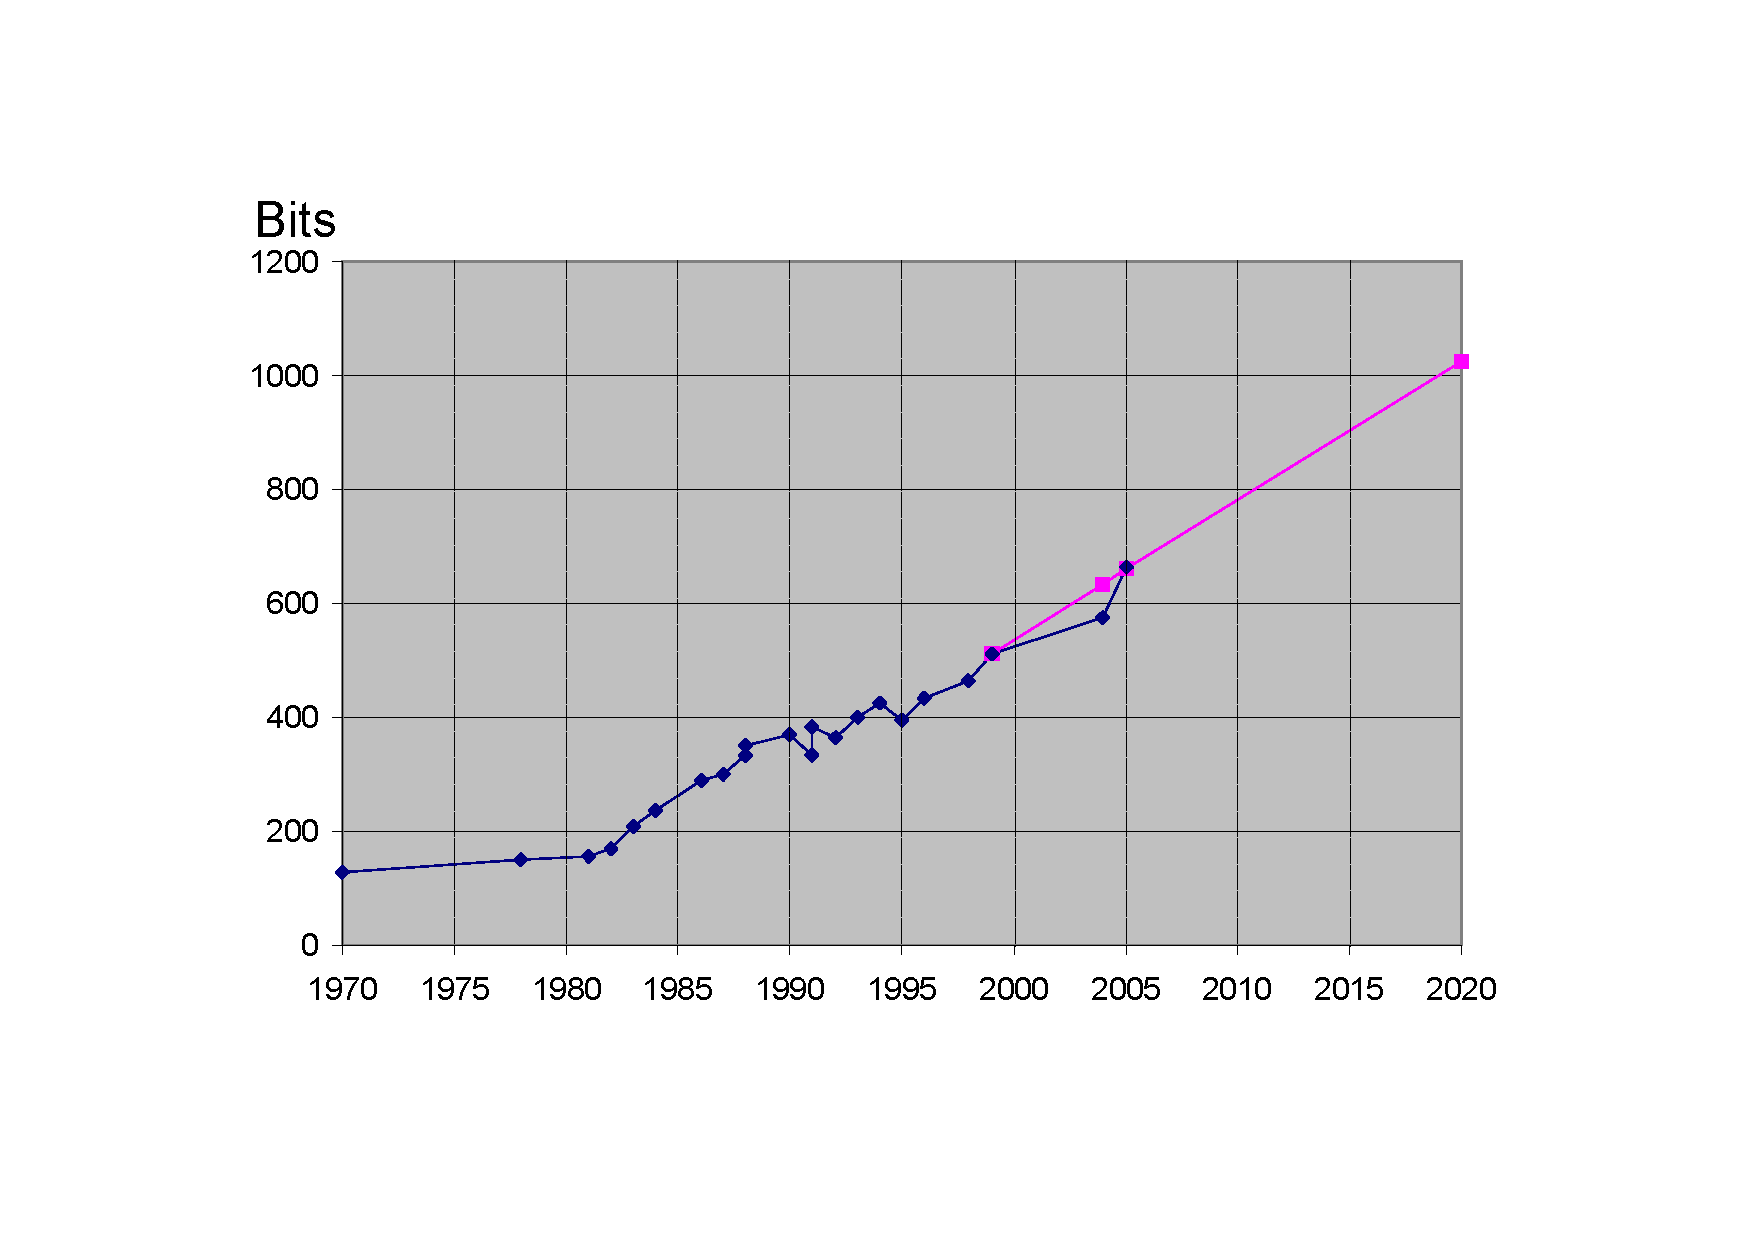
\includegraphics[scale=0.64, clip, viewport=-20 0 680 520]{figures/PrognoseRSAFaktorisierungSecorvo.pdf}
}
\caption{Forecast about future factorization records compared with current results
(from Secorvo)}
\label{secorvo-factorization-forecast}
\end{center}
\end{figure}



\clearpage
% ++++++++++++++++++++++++++++++++++++++++++++++++++++++++++++++++++++++++++
\vspace{4ex}
\begin{center}
\fbox{\parbox{15cm}{
    \emph{Hermann Hesse\footnotemark:}\\
    To let the possible happen, you again and again have to try the impossible.
}}
\end{center}
\addtocounter{footnote}{0}\footnotetext{%
  Hermann Hesse, German/Swiss writer and Nobel Prize winner, July 2, 1877 $-$ August 9, 1962.}
% ++++++++++++++++++++++++++++++++++++++++++++++++++++++++++++++++++++++++++

\subsection{Status regarding factorization of concrete large numbers}
\label{NoteFactorization}

An exhaustive overview about the factoring records
\index{Factorization!factoring records} of composed integers using different
methods can be found on the following web pages:
\vspace{-10pt}
\begin{itemize}
\item[]
     \href{http://www.crypto-world.com}
  {\texttt{http://www.crypto-world.com}} \\
     \href{http://www.tutorgig.com/ed/RSA\_number}
  {\texttt{http://www.tutorgig.com/ed/RSA\_number}}  ~~ The RSA Factoring Challenge \\
     \href{http://en.wikipedia.org/wiki/Integer_factorization_records}
  {\texttt{http://en.wikipedia.org/wiki/Integer\_factorization\_records}}
\end{itemize}
%\footnote{%
%This site was not quite up-to-date end of May 2005: RSA-200 was missing.}

The current record (as of May 2005) obtained using the GNFS method
(General Number Field Sieve) factorized a general 200 decimal digit into its
both prime factors.

\vskip +10pt
The last records\footnote{%
The 'RSA numbers' are certain large semiprime numbers (i.e., numbers with
exactly two prime factors)\index{Number!semi prime}. 
They were generated and published by the 
company RSA Security and they form the basis of the RSA Factoring 
Challenge, in which factorizations for these numbers are sought.
See \href{http://www.rsa.com/rsalabs/node.asp?id=2092}
 {\texttt{http://www.rsa.com/rsalabs/node.asp?id=2092}}.

The first RSA Factoring Challenge labeled the numbers, from RSA-100 
to RSA-500, according to their number of decimal digits; the second 
RSA Factoring Challenge labeled the numbers according to their number 
of binary digits. Within the second challenge cash prizes have been 
offered for successful factorizations of RSA576 to RSA2048 (RSA576, 
RSA640 etc. using 64 bit steps upwards).
An exception to this is RSA617, which was created prior to the 
change in the numbering scheme.

The researchers around Professor Jens Franke (from the University 
of Bonn, the GISA and the CWI) do not aim on getting cash prizes 
but in extending the research limits. So statements about the 
necessary length of a secure RSA modulus are more well-founded.

The 'C-numbers' originate from the Cunningham project:
\href{http://www.cerias.purdue.edu/homes/ssw/cun/}
     {\texttt{http://www.cerias.purdue.edu/homes/ssw/cun/}}
                                                               }
with factorization algorithms for composed numbers are
listed in the table~\ref{factorizationrecords}.

\begin{table}[h]
\begin{center}
\begin{tabular}{|c|cccc|}
\hline
	& {\bf Decimal digits} & {\bf Binary digits} & {\bf Factored on} & {\bf Factored by} \\
\hline
	C307 & 		307 & 1017 & May, 2007 & Jens Franke et al. \\
	RSA-200 & 	200 & 663 & May, 2005 & Jens Franke et al. \\
	RSA640\footnotemark & 	193 & 600 & November, 2005 & Jens Franke et al. \\
	C176 & 		176 & 583 & May, 2005 & Kazumaro Aoki et al. \\
	RSA576 & 	174 & 576 & December, 2003 & Jens Franke et al. \\
	RSA-160 & 	160 & 530 & April, 2003 & Jens Franke et al. \\
	C158 & 		158 & 523 & January, 2002 & Jens Franke et al. \\
	RSA-155	&	155 & 512 & August, 1999 & Herman te Riele et al. \\
\hline
\end{tabular}
\caption{The current factoring records (as of July 2009)}    % Eyecatcher_neue-Mersenne 
\label{factorizationrecords}
\end{center}
\end{table} 
\footnotetext{%
A research group of the GISA solved this challenge which was awarded with
20,000 US dollar using the GNFS method. The researchers needed about five
months to divide this number into its both 320 bit long prime factors.\\
RSA Labs offers its challenges since the beginning of the 1990th.
The next bigger challenge awarded with 30,000 US dollars is RSA-704.\\
See:
\href{http://www.heise.de/newsticker/meldung/print/65957}
{\texttt{http://www.heise.de/newsticker/meldung/print/65957}}
}

%be_2005: Erzwingen, dass die Abb. noch in diesem Kapitel !


Below the last records are explained in more detail.
The two methods, GNFS and SNFS, used to do so are shortly illustrated at the 
following web pages:
\index{General Number Field Sieve (GNFS)}
\index{Special Number Field Sieve (SNFS)}
\vspace{-10pt}
\begin{itemize}
\item[]
      \href{http://en.wikipedia.org/wiki/Special_number_field_sieve}
   {\texttt{http://en.wikipedia.org/wiki/Special\_number\_field\_sieve}} \\
      \href{http://en.wikipedia.org/wiki/General_number_field_sieve}
   {\texttt{http://en.wikipedia.org/wiki/General\_number\_field\_sieve}}
\end{itemize}
%\vspace{-10pt}



% --------------------------------------------------------------------------
\vskip +20pt
\paragraph{RSA-155} \label{RSA-155} \index{RSA-155}\mbox{}

On August 22, 1999 researchers from the Netherlands found the solution of this
RSA challenge. They factorized a 155-digit number into its both 78-digit primes
(see chapter~\ref{chptSecurityParam}). 

This 512 bit RSA-155 meant to reach a kind of {\em magic} border.


% --------------------------------------------------------------------------
\vskip +20pt
\paragraph{C158} \label{C158} \index{C158}\mbox{}
\hypertarget{C158-chap3}{}

On January 18, 2002 researchers at the German University of Bonn\footnote{%
\href{http://www.ercim.org/publication/Ercim\_News/enw49/franke.html, 2002-01}
{\texttt{http://www.ercim.org/publication/Ercim\_News/enw49/franke.html, 2002-01}}}
factorized a 158-digit decimal number into its both prime factors (these are
build with 73 and 86 decimal digits) using the GNFS method (General Number
Field Sieve)\index{General Number Field Sieve (GNFS)}.

This record got much less attention within the press than the solution of
RSA-155.

The task of the researchers from Bonn was not initiated by a challenge, but
they wanted to find the last prime factors of the integer $2^{953} - 1$
(see ``Wanted List'' of the Cunningham Project\index{Cunningham project}\footnote{%
Cunningham project: \href{http://www.cerias.purdue.edu/homes/ssw/cun/}
                 {\texttt{http://www.cerias.purdue.edu/homes/ssw/cun/}}}).

The 6 smaller prime factors, already found before have been:
$$
\begin{array}{c}
3, 1907, 425796183929, \\
1624700279478894385598779655842584377, \\
3802306738549441324432139091271828121 \quad {\rm and} \\
128064886830166671444802576129115872060027.
\end{array}
$$
The first 3 factors can be easily computed\footnote{%
E.g. using CrypTool\index{CrypTool} via menu 
{\bf Indiv. Procedures \textbackslash{} RSA Cryptosystem \textbackslash{} 
Factorization of a Number}. \\
CrypTool can factorize in a reasonable time numbers no longer than 250 bit.
Numbers bigger than 1024 bits are currently not accepted by CrypTool.
}.
The next three prime factors were found by P.~Zimmerman\footnote{%
\href{http://www.loria.fr/~zimmerma/ecmnet}{\tt http://www.loria.fr/\~{}zimmerma/ecmnet}}, 
T.~Grandlund\footnote{\href{http://www.swox.se/gmp/}{\tt http://www.swox.se/gmp/}}
and R. Harley during the years 1999 and 2000 using the elliptic curve factorization method.

The last remaining factor, called ``C158'', was known to be composite by
then, but its factors were not known (the following 3 lines contain one number):
$$
\begin{array}{c}
39505874583265144526419767800614481996020776460304936 \\
45413937605157935562652945068360972784246821953509354 \\
4305870490251995655335710209799226484977949442955603
\end{array}
$$
The factorization of C158 resulted in the following two 73- and 86-digit prime factors:
$$
\begin{array}{c}
3388495837466721394368393204672181522815830368604993048084925840555281177
\end{array}
$$
and
$$
\begin{array}{c}
1165882340667125990314837655838327081813101 \\
2258146392600439520994131344334162924536139.
\end{array}
$$
So now all 8 prime factors of $2^{953} - 1$ have been found.

\noindent\begin{minipage}{\textwidth}
\vspace{3ex}
Links:
\vspace{-10pt}
\begin{itemize}
\item[]   \href{http://www.loria.fr/~{}zimmerma/records/gnfs158}
       {\texttt{http://www.loria.fr/~{}zimmerma/records/gnfs158}} \\
          \href{http://www.crypto-world.com/FactorRecords.html}
       {\texttt{http://www.crypto-world.com/FactorRecords.html}} \\
          \href{http://www.crypto-world.com/announcements/c158.txt}
       {\texttt{http://www.crypto-world.com/announcements/c158.txt}}
\end{itemize}
\end{minipage}
\vspace{12pt}



% --------------------------------------------------------------------------
\vskip +20pt
\paragraph{RSA-160} \label{RSA-160} \index{RSA-160}\mbox{}
\hypertarget{RSA-160-chap3}{}

On January 18, 2002 researchers at the German University of Bonn\footnote{%
          \href{http://www.loria.fr/~zimmerma/records/rsa160}
       {\texttt{http://www.loria.fr/\~{}zimmerma/records/rsa160}} \\
          \href{http://www.loria.fr/~zimmerma/records/factor.html}
       {\texttt{http://www.loria.fr/\~{}zimmerma/records/factor.html}} \\
          \href{http://www.crypto-world.com/FactorWorld.html}
       {\texttt{http://www.crypto-world.com/FactorWorld.html}}
} 
factorized a 160-digit number into its both prime factors (these are build
with each 80 decimal digits) using the GNFS method (General Number Field
Sieve)\index{General Number Field Sieve (GNFS)}.

The  computations for the factorization of RSA-160 also took place at the 
German Information Security Agency (GISA) in Bonn\footnote{%
Every year the GISA\index{GISA} creates a paper to describe which 
crypto algorithms are feasible to generate digital signatures according
to the German signature law -- under participation of experts from
economy and science. To review signature methods based on the
factorization problem the GISA also co-operates with researchers from the
University of Bonn.
Further information about crypto algorithms can be found on the web page of GISA:
   \href{http://www.bsi.bund.de/esig/basics/techbas/krypto/index.htm}
{\texttt{http://www.bsi.bund.de/esig/basics/techbas/krypto/index.htm}}.
}.

The 160-digit decimal number origins from the old challenge list of RSADSI.
This number was retracted after RSA-155 (RSA512) had been factorized 
successfully. The prime factors of RSA-160 were still unknown.
So this record of the team of Prof.\ Franke provides the solution of 
the old challenge, for which RSADSI didn't award a price anymore.

The composite number called ``RSA-160'' is (the following 3 lines contain
one number):
$$
\begin{array}{c}
215274110271888970189601520131282542925777358884567598017049 \\
767677813314521885913567301105977349105960249790711158521430 \\
2079314665202840140619946994927570407753
\end{array}
$$
The factorization of RSA-160 resulted in the following two prime factors:
$$
\begin{array}{c}
p = 45427892858481394071686190649738831 \\         
    656137145778469793250959984709250004157335359
\end{array}
$$
and
$$
\begin{array}{c}
q = 47388090603832016196633832303788951 \\
    973268922921040957944741354648812028493909367
\end{array}
$$

The calculations took place between December 2002 and April 2003.
% \vspace{12pt}
\vspace{24pt}



% --------------------------------------------------------------------------
\vskip +20pt
\hypertarget{RSA-200-chap3}{}
\paragraph{RSA-200} \label{RSA-200} \index{RSA-200}\mbox{}
%\hypertarget{RSA-200-chap3}{}

On May 9, 2005 the research group of Prof. Jens Franke at the German
University of Bonn\footnote{%
   \href{http://www.loria.fr/~zimmerma/records/rsa200}
{\texttt{http://www.loria.fr/\~{}zimmerma/records/rsa200}}} announced,
that they achieved a new world record in number factorization
together with their colleagues of the Amsterdam Centrum voor Wiskunde
en Informatica. 

They factorized a 200-digit number into its both prime factors 
(these are build with each 100 decimal digits) using the GNFS method 
(General Number Field Sieve)\index{General Number Field Sieve (GNFS)}.

The composite number called ``RSA-200'' is (the following 3 lines contain
one number):
$$
\begin{array}{c}
2799783391122132787082946763872260162107044678695542853756000992932 \\
6128400107609345671052955360856061822351910951365788637105954482006 \\
576775098580557613579098734950144178863178946295187237869221823983
\end{array}
$$
The factorization of RSA-200 resulted in the following two prime factors:
$$
\begin{array}{c}
p = 35324619344027701212726049781984643686711974001976 \\         
    25023649303468776121253679423200058547956528088349
\end{array}
$$
and
$$
\begin{array}{c}
q = 79258699544783330333470858414800596877379758573642 \\
    19960734330341455767872818152135381409304740185467
\end{array}
$$

The calculations took place between December 2003 and May 2005.
The factorization done by the group around Bahr, B\"ohm, Franke, Kleinjung, 
Montgomery and te Riele lasted almost 17 months.
The operating expense of the calculations was about 120,000 
MIPS-years\footnote{%
A MIPS-year (MY) is the quantity of operations a machine can perform in one year,
if the machine constantly achieves one million integer operations per second (MIPS).
For illustration: a INTEL Pentium 100 processor achieves about 50 MIPS.
To factorize a 2048 bit module it is estimated to need about {$8.5 \cdot
 10^{40}$ MY}. }.
\vspace{24pt}





% --------------------------------------------------------------------------
\vskip +20pt
\paragraph{C307 / M1039} \label{C307} \index{C307} \index{M1039}\mbox{}
\hypertarget{C307-chap3}{}

In May 2007 Prof. Franke, Prof. Kleinjung (University of Bonn),
the Japanese telecommunication company NTT and Prof. Arjen Lenstra
(Polytechnical University of Lausanne) announced, that they managed to
factorize a $307$ digit decimal number into its both prime factors
with the SNFS method (Special Number Field Sieve)
\index{Special Number Field Sieve (SNFS)} within 11 months
(the two factors have 80 and 227 decimal digits).

The task of the researchers was not initiated by a challenge, but
they wanted to find the last prime factors of the Mersenne number $2^{1039}+1$
(see ``Wanted List'' of the Cunningham Project\index{Cunningham project}\footnote{%
Cunningham project: \href{http://www.cerias.purdue.edu/homes/ssw/cun/}
                 {\texttt{http://www.cerias.purdue.edu/homes/ssw/cun/}}\\
Cunningham table: \href{http://homes.cerias.purdue.edu/~ssw/cun/pmain1206}
                {\texttt{http://homes.cerias.purdue.edu/\~{}ssw/cun/pmain1206}}\\
The numbers in the Cunningham table have the following syntax:\\
``(2,n)-'' means $2^{n}-1$;~~~
``(2,n)+'' means $2^{n}+1$.\\
To describe the magnitude one writes $p<n>$ or $c<n>$: 
``n'' is the number of decimal digits and ``p'' and ``c'' tell,
whether the number is prime or composite.\\
$2^{1039}-1 = p7 * c307 = p7 * p80 * p227$ \\
It is explained more precisely at the CUN page:\\
``2651+ means $2^{651} + 1$ and the size (c209 means 209 decimal digits)
of the
number which was factored.  Then come the new factor(s), the discoverer and
the method used.  Recently, only the multiple polynomial quadratic sieve
(ppmpqs), the elliptic curve method (ecm) and the number field sieve (nfs)
have been used.  `hmpqs' stands for hypercube multiple polynomial quadratic
sieve.  Under `new factors', `p90' means a 90-digit prime and `c201' is a
201-digit composite number.''.
}).\\


The number $2^{1039}-1$ consists of 3 prime factors: The smallest one, 
$p7 = 5080711$ was already known.\footnote{%
This one can also be found using CrypTool\index{CrypTool}  via menu 
{\bf Indiv. Procedures \textbackslash{} RSA Cryptosystem \textbackslash{} 
Factorization of a Number} --- with the algorithms of Brent, Williams or
Lenstra, which are ``relatively'' good to separate small factors. \\
CrypTool can factorize in a reasonable time numbers no longer than 250 bit.
}


To complete this the second factor (co-divider) ``C307'' had to be factorized:
Till then it was only known, that the last remaining factor was composite,
but it was unknown, how many prime factors it had and what are the prime factors.
The following 5 lines contain one number:
$$
\begin{array}{c}
C307 =1159420574072573064369807148876894640753899791702017724986868353538\\
8224838599667566080006095408005179472053993261230204874402860435302\\
8619141014409345351233471273967988850226307575280937916602855510550\\
0425810771176177610094137970787973806187008437777186828680889844712\\
822002935201806074755451541370711023817
\end{array}
$$
The factorization of C307 resulted in the following two 80- and 2276-digit prime factors:
$$
\begin{array}{c}
p80 = 558536666199362912607492046583159449686465270184\\
      88637648010052346319853288374753
\end{array}
$$
and
$$
\begin{array}{c}
p227 = 207581819464423827645704813703594695162939708007395209881208\\
       387037927290903246793823431438841448348825340533447691122230\\
       281583276965253760914101891052419938993341097116243589620659\\
       72167481161749004803659735573409253205425523689
.
\end{array}
$$
So now the number $2^{1039}-1$ is completely factorized in its 3 prime factors.

\noindent\begin{minipage}{\textwidth}
\vspace{3ex}
Links:
\vspace{-10pt}
\begin{itemize}
\item[]   \href{http://www.loria.fr/~zimmerma/records/21039-}
       {\texttt{http://www.loria.fr/\~{}zimmerma/records/21039-}} \\
          \href{http://www.crypto-world.com/announcements/m1039.txt}
       {\texttt{http://www.crypto-world.com/announcements/m1039.txt}} \\
          \href{http://www.crypto-world.com/FactorAnnouncements.html}
       {\texttt{http://www.crypto-world.com/FactorAnnouncements.html}} \\
          \href{http://www1.uni-bonn.de/pressDB/jsp/pressemitteilungsdetails.jsp?detailjahr=2007&detail=160}
       {\texttt{http://www1.uni-bonn.de/pressDB/jsp/pressemitteilungsdetails.jsp?}} \\
          \href{http://www1.uni-bonn.de/pressDB/jsp/pressemitteilungsdetails.jsp?detailjahr=2007&detail=160}
       {\texttt{\quad \quad \quad detailjahr=2007\&detail=160}}\end{itemize}
\end{minipage}






% --------------------------------------------------------------------------
\vskip +70pt
\paragraph{Size of factorized numbers compared to primality proven numbers}
\mbox{}

As you notice the factorized compound numbers built of 2 prime factors are
much smaller than the especially structured numbers, for which primality 
tests\index{Primality testing} are able to decide whether these numbers are prime 
or not (see chapters~\ref{search_for_very_big_primes},~\ref{primality_tests}
and \ref{spezialzahlentypen}). 

% be_2005_UPDATEN_if-new-mersenne-prime-appears % Eyecatcher_neue-Mersenne
Length in bits of the current world records:\\
% (RSA-200 $\longleftrightarrow{}$ 43rd known Mersenne prime) \\
%  ~  $663 \longleftrightarrow 30,402,457$.
%$$ (RSA-200 ~~ \longleftrightarrow{} ~~ 43rd ~known~Mersenne~Prime) $$ mnmnmn
%$$ (RSA~-200 ~~ \longleftrightarrow{} ~~ 43rd ~known~Mersenne~Prime) $$
$$ [RSA{-}200~Number] ~~\longleftrightarrow{}~~ [43rd ~known~Mersenne~Prime] $$
$$ 663 ~~ \longleftrightarrow{} ~~ 30,402,457 ~~~~~$$




% --------------------------------------------------------------------------
\vskip +60pt
\subsection{Further current research about primes and factorization}
\label{FactorizationResearch}
Prime numbers are part of very many topical research areas in number theory
and computer science. Progress made with factorization is bigger than was
estimated 5 years ago -- this is not only due to faster computers but
also new knowledge.

The security of the RSA algorithm is based on the empirical observation
that factoring large numbers is a hard problem. A module $n$ (typically,
1024 bit) can be easily constructed as the product of two large primes $p$,
$q$ (typically, 500$-$600 bit each), by calculating $n=pq$. However, it is
a hard problem to extract $p$, $q$ from $n$.  Without knowing $p$ or $q$,
the private key cannot be calculated.

Thus, any progress in efficiency of factorizing large integers will effect the
security of the RSA. As a consequence, the underlying primes $p$, $q$ and,
thus, the module n (1024 bit as of today) have to be increased. In case of a
quantum leap in factorization, the RSA algorithm might be compromised.


% --------------------------------------------------------------------------
\vskip +20pt
\paragraph{Bernstein's paper and its implication on the
  security of the RSA algorithm}
\label{RSABernstein} \index{Factorization!factorization problem}\mbox{}

In his paper ``Circuits for integer factorization: a proposal'' 
(\href{http://cr.yp.to/djb.html}{\texttt{http://cr.yp.to/djb.html}}),
published November 2001, D.~J.\ Bernstein \cite{nt:Bernstein2001} 
addresses the problem of
factorizing large integers. Therefore, his results are of relevance from a
RSA point of view.  As a main result Bernstein claims that the
implementation of the General Number Field Sieve algorithm (GNFS)
 \index{General Number Field Sieve (GNFS)} can be improved to factor, with
the same effort as before, integers with three times more digits.

We note that the definition of \emph{effort} is a crucial point: Bernstein
claims that effort is the product of time and costs of the machine
(including the memory used). The gist of the paper lies in the fact that he
can reduce a big part of factorizing to sorting. Using Schimmler's scheme,
sorting can be optimized by massive parallel computing.  At the end of
section 3 Bernstein explains this effect: The costs of $m^2$ parallel
computers with a constant amount of memory is a constant times $m^2$.  The
costs of a computer with a single processor and memory of size $m^2$ is
also of the order of $m^2$, but with a different constant factor.  With
$m^2$ processors in parallel, sorting of $m^2$ numbers (with Schimmler's
scheme) can be achieved in time $m$, while a $m^2$-memory computer needs
time of the order of $m^2$. Decreasing memory and increasing the number of
processors, the computing time can be reduced by a factor $1/m$ without
additional effort in terms of total costs.  In section 5 it is said that
massive parallel computing can also increase efficiency of factorizing
using Lenstra's elliptic-curve-method (a search algorithm has costs that
increase in a quadratic square manner instead of cubically).

We note that all results achieved so far are asymptotic results. This means
that they only hold in the limit n to infinity. Unfortunately, there is no
upper limit for the residual error (i.e. the difference between the real
and the asymptotic value) for finite n --- a problem which has already been
addressed by the author. As a consequence, one cannot conclude whether the
costs (in the sense of Bernstein) for factorizing 1024$-$2048-bit RSA modules
can be significantly reduced.

There is no doubt that Bernstein's approach is innovative. However, the
reduction of computing time under constant costs comes along with a massive
use of parallel computing --- a scenario which seems not to be realistic
yet. For example, formally 1 sec computing time on one machine and
1/1,000,000 sec time parallel computing time on 1,000,000 machines might
have same costs.  In reality, it is much harder to realize the second
situation, and Bernstein does not take into account the fixed costs, in
particular for building a network between all these computers.

Although distributed computing over a large network might help to overcome
this problem, realistic costs for data transfer have to be taken into
account --- a point which was not addressed in Bernstein's proposal.

As long as there is neither (low cost) hardware nor a distributed computing
approach (based on Bernstein's ideas), there should not be a problem for
RSA. It has to be clarified from which magnitude of n on Bernstein's method
could lead to a significant improvement (in the sense of the asymptotic
result). 

Arjen Lenstra, Adi Shamir et. al. analyzed the paper of Bernstein
\cite{nt:Lenstra2002}.  In summary they expect a factorization improvement on
how much longer the bit length of the keys could be with a factor of 1.17
(instead of factor 3 as proposed by Bernstein).

The abstract of their paper ``Analysis of Bernstein's Factorization
Circuit'' says:

``... Bernstein proposed a circuit-based implementation of the matrix
step of the number field sieve factorization algorithm. We show that under
the non-standard cost function used in [1], these circuits indeed offer an
asymptotic improvement over other methods but to a lesser degree than
previously claimed: for a given cost, the new method can factor integers
that are 1.17 times larger (rather than 3.01).  We also propose an improved
circuit design based on a new mesh routing algorithm, and show that for
factorization of 1024-bit integers the matrix step can, under an optimistic
assumption about the matrix size, be completed within a day by a device
that costs a few thousand dollars.  We conclude that from a practical
standpoint, the security of RSA relies exclusively on the hardness of the
relation collection step of the number field sieve.''

\href{http://www.rsasecurity.com/}{RSA Security's} analysis of the Bernstein
paper \cite{nt:RSA Security 2002} from April, 8 2002 also -- as expected --
concludes, that RSA is still not compromised.

This is still an ongoing discussion.

When this section was written (June 2002) nothing was publicly known about, how
far there exist implementations of his theoretical onsets and how much
financing there was for his research project.

\vskip +12pt
\noindent\begin{minipage}{\textwidth}
Links:
\vspace{-10pt}
\begin{itemize}
  \item[] \href{http://cr.yp.to/djb.html}
               {\texttt{http://cr.yp.to/djb.html}} \\
          \href{http://www.counterpane.com/crypto-gram-0203.html\#6}
               {\texttt{http://www.counterpane.com/crypto-gram-0203.html\#6}} \\
          \href{http://www.math.uic.edu}
               {\texttt{http://www.math.uic.edu}}
\end{itemize}
\end{minipage}


% --------------------------------------------------------------------------
\vskip +20pt
\paragraph{The TWIRL device} \label{TWIRLDevice} \index{TWIRL device}\mbox{}

In January 2003 Adi Shamir and Eran Tromer from the Weizmann Institute of Science published a preliminary draft called {\em ``Factoring Large Numbers with the TWIRL Device''} raising concerns about the security of key sizes till 1024 bits \cite{nt:Shamir2003}. 

Their abstract summarizes their results very well: ``The security of the RSA
cryptosystem depends on the difficulty in factoring large integers. The best
current factoring algorithm is the Number Field Sieve (NFS), and its most
difficult part is the sieving step. In 1999 a large distributed computation
involving thousands of workstations working for many months managed to factor a
512-bit RSA key, but 1024-bit keys were believed to be safe for the next 15-20
years. In this paper we describe a new hardware implementation of the NFS
sieving step ... which is 3-4 orders of magnitude more cost effective than the
best previously published designs ... . Based on a detailed analysis of all the
critical components (but without an actual implementation), we believe that the
NFS sieving step for 1024-bit RSA keys can be completed in less than a year with
a \$10M device, and that the NFS sieving step for 512-bit RSA keys can be
completed in less than ten minutes with a \$10K device. Coupled with recent
results about the difficulty of the NFS matrix step ... this raises some
concerns about the security of these key sizes.''

A detailed explanation from these two authors also can be found in the
RSA Laboratories CryptoBytes \cite{nt:Shamir2003a}.

The 3-page article in the DuD issue of June 2003 \cite{nt:Weis2003} contains
a very good explanation, how the attack using the Generalized Number Field
Sieve (GNFS) \index{General Number Field Sieve (GNFS)} works and which 
progress is made, to factorize numbers.
At GNFS we can distinguish 2 general steps: 
The sieve step (relation collecting) and the matrix reduction.
Besides the sieve step is highly parallelizable, it dominates the overall
calculation burden. Shamir and Tromer haven't built a TWIRL device yet,
but the estimated costs of 10 till 50 million Euro (in order to factorize
a 1024-bit number) is not prohibitive for secret agencies or big criminal
organizations, because the ``costs for a single espionage satellite is
estimated e.g. to be several billion USD''. The authors therefore
recommend, to get as soon as possible rid of today used sensible RSA, 
Diffie-Hellman or ElGamal keys up to 1024 bit and to use then keys of at
least 2048 bit length.
The planned TCPA/Palladium hardware \index{Palladium} will use 2048-bit
RSA keys!

So recommendations like the ones from the GISA (German Information Security Agency) to use higher key lengths are very valid.


% --------------------------------------------------------------------------
\vskip +20pt
\paragraph{``Primes in P'': Primality testing is polynomial} \label{PrimesinP} 
\index{Primality testing}\mbox{}

In August 2002 the three Indian researchers M. Agrawal, N. Kayal and N. Saxena published the paper {\em ``PRIMES in P''} about a new primality testing algorithm called AKS\index{AKS} \cite{nt:Agrawal2002}. 
They discovered a polynomial\index{Polynomial} time deterministic algorithm for determining if a number is prime or not.

The importance of this discovery is that it provides number theorists with new insights and opportunities for further research. Lots of people over centuries have been looking for a polynomial time test for primality, and this result is a major theoretic breakthrough. It shows that new results can be generated from already known facts.

But even its authors note that other known algorithms may be faster (for example ECPP). The new algorithm works on any integer. For example the GIMPS project uses the Lucas-Lehmer primality test which takes advantage of the special properties of Mersenne numbers. This makes the Lucas-Lehmer test much faster, allowing to test numbers with millions of digits while general purpose algorithms are limited to numbers with a few thousand digits.

\noindent Current research results on this topic can be found at:
\vspace{-10pt}
\begin{itemize}
  \item[] \href{http://www.mersenne.org/}
               {\texttt{http://www.mersenne.org/}} \\
          \href{http://fatphil.org/maths/AKS/}
               {\texttt{http://fatphil.org/maths/AKS/}} Original paper in English\\
          \href{http://ls2-www.cs.uni-dortmund.de/lehre/winter200203/kt/material/primes.ps}
               {\texttt{http://ls2-www.cs.uni-dortmund.de/lehre/winter200203/kt/material/primes.ps}}\\
	       \hspace*{2em}Good explanation in German by Thomas Hofmeister. 
\end{itemize}
\vskip +10 pt





% ++++++++++++++++++++++++++++++++++++++++++++++++++++++++++++++++++++++++++
% \vskip +40 pt
\newpage
\begin{center}
\fbox{\parbox{15cm}{{\em Joanne\index{Rowling, Joanne} K. Rowling\footnotemark:}\\
It is our choices, that show what we truly are, far more than our abilities.}}
\end{center}

\addtocounter{footnote}{0}\footnotetext{Joanne K. Rowling, ~``Harry Potter and the Chamber of Secrets'', Bloomsbury, 1998, 
last chapter ``Dobby's reward'', p.~245, by Dumbledore.}

%\begin{quote}
%{\em Joanne K. Rowling}\footnote{Joanne K. Rowling, ~``Harry Potter and the Chamber of Secrets'', Carlsen, 1998, 
%last chapter ``Dobby's reward'', p.~343.}:\\
%It is our choices, that show what we truly are, far more than our abilities.
%\end{quote}

% ++++++++++++++++++++++++++++++++++++++++++++++++++++++++++++++++++++++++++
\section{Applications of asymmetric cryptography using numerical examples}

The results of modular arithmetic are used extensively in \index{Cryptography!modern} modern cryptography. Here we will provide a few examples from 
cryptography using small\footnote{In the RSA procedure, we call numbers ``small'' if the bit lengths are much less than $1024$ 
bits (i.e. $308$ decimal points). In practice, $1024$ bits is currently the minimum length for a secure Certification 
Authority RSA modulus.} numbers.

Enciphering a text entails applying a function (mathematical operation) to a character string (number) to generate a 
different number. Deciphering entails reversing this function, in other words using the distorted image that the function 
has created from the plaintext in order to restore the original image. For example, the sender could take the plaintext 
$M$ of a confidential message and add a secret number, the key $S$, to obtain the cipher text $C$:
$$C = M + S.$$
The recipient can reconstruct the plaintext by reversing this operation, in other words by subtracting $S$:
$$M = C - S.$$
Adding $S$ reliably makes the plaintext impossible to read. However, this encryption is rather weak, because all an 
interceptor needs to do to calculate the key is obtain a plaintext and the associated cipher text
$$S = C - M,$$
and can then read any subsequent messages encrypted using $S$. \\
The essential reason for this is that subtraction is just as simple an operation as addition. 


% --------------------------------------------------------------------------
\hypertarget{OneWayFunktion2}{}%
\subsection{One way functions}\index{One way function}
\label{OneWayFunktion2}%
If the key is to be impossible to determine even with knowledge of both the 
plaintext and the cipher text, we need a function that is, on the one hand, 
relatively easy to calculate -- we don't want to have problems encrypting 
messages. On the other hand, the inverse function should exist (otherwise 
information would be lost during encryption), but should be de facto 
incalculable.

What are possible candidates for such a {\bf one way function}? We could take multiplication rather than addition, 
but even primary school children know that the inverse function, division, is only slightly more difficult than multiplication 
itself. We need to go one step higher in the hierarchy of calculation methods. It is still relatively simple to calculate the 
power of a number, but the corresponding two reverse functions -- {\em taking roots} (find $b$ in the equation $a = b^c$  when $a$ 
and $c$ are known) and {\em calculating logarithms} (find $c$ in the above equation when $a$ and $b$ are known) are so complicated 
that pupils normally do not learn them at school.

Although a certain structure can still be recognised for addition and multiplication, raising numbers to the power of 
another or calculating exponentials totally mixes up all the numbers. Knowing a few values of the function doesn't tell 
us much about the function as a whole (in contrast to addition and multiplication).


% --------------------------------------------------------------------------
\subsection{The Diffie-Hellman key exchange protocol}
\index{Diffie, Whitfield} 
\index{Hellman, Martin} 
\index{Key agreement (key exchange)!Diffie-Hellman}
\index{Diffie-Hellman}

Whitfield Diffie, Martin E. Hellman and Ralph Merkle developed this DH key 
exchange protocol in Stanford in 1976\footnote{%
With CrypTool\index{CrypTool} this exchange protocol has been
visualized: you can execute the single steps with concrete numbers using 
menu {\bf Indiv. Procedures \textbackslash{} Protocols
\textbackslash{} Diffie-Hellman Demonstration}.
}.

Alice and Bob\footnote{Bob\index{Bob} and Alice\index{Alice} are the default
names used for the two authorized participants in a protocol (see
\cite[p. 23]{nt:Schneier1996nt}).
} use a one way function to obtain a key $S$, the session key, for subsequent
correspondence. This is then a secret that is only known to the two of them.
Alice selects a random number $a$ and keeps it secret. She applies a one way
function to $a$ to calculate the number $A = g^a$ and sends it to Bob. He does
the same, by selecting a secret random number $b$, calculating $B = g^b$ and
sending it to Alice. The number $g$ is random and can be publicly known.
Alice applies the one way function together with her secret number $a$ to
$B$, while Bob does the same with his secret number $b$ and the received
number $A$.

The result $S$ is the same in each case because the one way function is
commutative: $(g^a)^b = (g^b)^a$. But even Bob cannot reconstruct Alice's
secret number $a$ from the data available to him, while Alice cannot
determine Bob's secret number $b$. And a perpetrator who knows $g$ and
has intercepted both $A$ and $B$ cannot use this knowledge to 
determine $a, b$ or $S$.

\vskip +10 pt
\input{figures/DH-en.latex}
\vskip +10 pt


{\bf Procedure:}

\noindent Alice and Bob want to negotiate a secret session key $S$ via a channel that may be intercepted. 
\begin{itemize}
\item[{\bf 1.}] They select a prime number $p$ and a random number $g$ and exchange this information openly.
\item[{\bf 2.}] Alice now selects $a$, a random number less than $p$ and keeps it secret.

                Similarly, Bob selects $b,$ a random number less than $p$ and keeps it secret.
\item[{\bf 3.}] Alice now calculates $A \equiv g^a {\rm ~(mod~} p)$.\\
                Bob calculates $B \equiv g^b {\rm ~(mod~} p)$.
\item[{\bf 4.}] Alice sends the result $A$ to Bob.\\
                Bob sends the result $B$ to Alice.
\item[{\bf 5.}] In order to now determine the session key to be used by both,
                they both separately raise the respective results they have
                received to the power of their secret random number modulo $p$.
                This means: 
\begin{itemize}
    \item[-] Alice calculates $S \equiv B^a {\rm ~(mod~} p)$ and
    \item[-] Bob calculates $S \equiv A^b {\rm ~(mod~} p)$.
\end{itemize}
\end{itemize}
Even if a spy intercepts $g, p$, and the interim results $A$ and $B$, he cannot
use these in order to determine the used session key used -- due to the
difficulty of calculating the discrete logarithm\footnotemark.
\footnotetext{%
Further details about
the\index{Logarithm problem!discrete}\index{Discrete logarithm}
\hyperlink{HT-Discrete-Logarithm-as-Basis}{discrete logarithm problem}
can be found in chapter~\ref{L-Discrete-Logarithm-as-Basis}.
}

\vskip + 5pt
\noindent We will now use an example with (unrealistically) small numbers to illustrate this.
\vskip +1em

\begin{example}{ using small numbers:}
\begin{itemize}
\item[{\bf 1.}] Alice and Bob select $g = 11, p = 347$.
\item[{\bf 2.}] Alice selects $a = 240$, Bob selects $b = 39$ and they keep $a$ and $b$ secret.
\item[{\bf 3.}] Alice calculates $A \equiv g^a \equiv 11^{240}  \equiv 49 {\rm ~(mod~} 347).$\\
                Bob calculates $B \equiv g^b \equiv 11^{39} \equiv 285 {\rm ~(mod~} 347).$
\item[{\bf 4.}] Alice sends Bob:   $A \equiv 49$,\\
                Bob sends Alice: $B \equiv 285$.
\item[{\bf 5.}] Alice calculates $B^a \equiv 285^{240} \equiv 268 {\rm ~(mod~} 347),$\\
                Bob calculates $A^b \equiv   49^{39} \equiv 268 {\rm ~(mod~} 347).$
\end{itemize}
Alice and Bob can now communicate securely using their shared session key. Even if spies were to intercept everything 
transferred via the connection:
$g = 11, p = 347, A = 49$ and $B = 285$, they would not be able to calculate the secret key.
\end{example}

\begin{remark}{:}\\
In this example using such small numbers, it is easily possible to calculate the discrete
logarithms, but with large numbers the discrete logarithm\index{Discrete logarithm}
problem\footnote{%
You can use Sage to determine the discrete logarithm $x$ that solves the
equation $11^x \equiv 49 \pmod{347}$ (here for Alice)\index{Sage}:
\texttt{discrete\_log(mod(49, 347), mod(11, 347))}. The returned value
is $67$.\\
Such number theoretic tasks can also be solved using other
tools like PariGP\index{Pari-GP}, LiDIA\index{LiDIA}, BC\index{BC} or
Mathematica\index{Mathematica}
(see the list of web sites in the appendix at the end of this chapter):\\
- Pari-GP: \texttt{znlog(Mod(49,347),Mod(11,347))}.\\
- LiDIA:   \texttt{dl(11,49,347)}.\\
- Mathematica: The general Solve function delivers the {em tdep message} ``The equations
  appear to involve the variables to be solved for in an essentially non-algebraic way''.\\
- Mathematica: {\tt MultiplicativeOrder[11, 347, 49]}.\\
All deliver the result $67$.
}${}^,$\footnote{%
Why have the functions delivered the value $67$ for the discrete
logarithm\index{Discrete logarithm} of Alice rather than $240$ which Alice
selected as exponent $a$?\\
The discrete logarithm is
the smallest natural exponent that solves the equation 
$11^x \equiv 49 \pmod{347}$. Both $x = 67$ and $x = 240$ (the number
selected in the example) satisfy the equation and can therefore be
used to calculate the session key: 
$285^{240} \equiv 285^{67} \equiv 268 \pmod{347}$.
If Alice and Bob
had selected a primitive root\index{Primitive root} modulo $p$ as base $g$, then for every
remainder from the set $\{1, 2, \dots, p-1 \}$ there is exactly one
exponent from the set $\{0, 1, \dots, p-2 \}$. \\
\indent As an aside, there are $172$ different primitive roots modulo $347$,
$32$ of which are prime (not necessary). Since the number $11$
selected for $g$ in the example is not a primitive root\index{Primitive root} of $347$, the
remainders do not take all values from the set $\{1, 2, \dots, 346 \}$. 
Thus, for a particular remainder there may be more than one exponent
or even no exponent at all in the set $\{0, 1, \dots, 345 \}$ that
satisfies the equation.\\
With the relevant Sage\index{Sage} commands you find:\\
\texttt{is\_prime(347)=True}, \texttt{euler\_phi(347)=346}, \texttt{gcd(11,347)=1} and 
\texttt{multiplicative\_order(mod(11, 347))=173}.

\begin{tabular}{|c|c|l|}
\hline
i  & $11^i \bmod 347$ & \\
\hline
      0  &          1   &  \\
      1  &         11   &  \\                                     
      2  &        121   &  \\                                     
      3  &        290   &  \\                                     
     67  &         49   & searched exponent \\                    
    172  &        284   &  \\                                                  
    173  &          1   &= multiplicative order of $11^i \bmod 347$ \\ 
    174  &         11   &  \\                                                     
    175  &        121   &  \\                                     
    176  &        290   &  \\                                     
    240  &         49   & searched exponent \\
\hline
\end{tabular}
\vskip +6 pt

Further information concerning \hyperlink{AppArith3a2}{primitive roots\index{Primitive root}}
can be found in appendix E of this chapter. %\ref{primitive-roots-with-sage}. xxxxxprro
% appendix E eigentlichnicht gut, aber~\ref{primitive-roots-with-sage}. liefert 4.13.5!  xxxxxprro

} is extremely difficult to solve.
\end{remark}

\noindent To get the discrete logarithms, here we need to calculate:\\
For Alice: $11 ^ x \equiv 49 {\rm ~(mod~}347)$, that means $\log_{11}(49) {\rm ~(mod~}347).$\\
For Bob: $11 ^ y \equiv 285 {\rm ~(mod~}347)$, that means $\log_{11}(285){\rm ~(mod~}347)$.



% ++++++++++++++++++++++++++++++++++++++++++++++++++++++++++++++++++++++++++
\newpage
\hypertarget{Chapter_ElementaryNT_12}{}
\section[The RSA procedure with actual numbers]{The RSA procedure with actual numbers\footnotemark}
\footnotetext{%
    \index{Sage}%
    \index{Minh Van Nguyen}%
    Additional material: Minh Van Nguyen, ``Number Theory and the RSA
    Public Key Cryptosystem'', 2009. An introductory tutorial on using
    Sage to study elementary number theory and public key
    cryptography. A didactically very clear article about some basic
    number theory and Sage usage. 
    \href{http://nguyenminh2.googlepages.com/numtheory-crypto-sage.pdf}
    {\url{http://nguyenminh2.googlepages.com/numtheory-crypto-sage.pdf}}.
}
\label{rsaconcrete}\index{RSA}
Having described above \hyperlink{RSA}{how the RSA procedure works}, we will now work through the steps using actual, but small, numbers.


% --------------------------------------------------------------------------
\subsection{RSA with small prime numbers and with a number as message}

Before applying the RSA procedure to a text, we will first demonstrate it
directly using a single number as message\footnote{Using CrypTool\index{CrypTool} you can solve this with the menu 
{\bf Indiv. Procedures \textbackslash{} RSA Cryptosystem \textbackslash{} RSA Demonstration}.}.
\begin{itemize}
\item[{\bf 1.}] Let the selected prime numbers be $p=5$ and $q=11$. \\
Thus, $n=55$ and $J(n)=(p-1)*(q-1)=40$.
\item[{\bf 2.}] $e = 7$ (should\footnote{%
                See footnote~\ref{foot:Selection-of-e} on page
                \pageref{foot:Selection-of-e}.}
                lie between $11$ and $39$ and must be relatively prime
                to $40$).
\item[{\bf 3.}] $d = 23$ (since $23*7 \equiv 161 \equiv 1{\rm ~(mod~} 40)$),
    \begin{itemize}
    \item[] $\rightarrow$ Public key of the recipient:  $(55, 7),$
    \item[] $\rightarrow$ Private key of the recipient: $(55, 23).$
    \end{itemize}
\item[{\bf 4.}] Let the message be the number $M = 2$ (so no division into blocks is required).
\item[{\bf 5.}] Encryption: $C \equiv 2^7 \equiv 18 {\rm ~(mod~}55).$
\item[{\bf 6.}] The cipher text is simply the number $C = 18$ (we therefore do not need to divide it into blocks).
\item[{\bf 7.}] Decryption: 
        $M \equiv 18^{23} \equiv 18^{(1+2+4+16)} \equiv 18*49*36*26 \equiv 2 {\rm ~(mod~}55).$
\end{itemize}


We will now apply the RSA procedure to a text, first using the upper case alphabet ($26$ characters), then using the entire ASCII character set as the basis for the messages.


% --------------------------------------------------------------------------
\subsection[RSA with slightly larger primes and an upper-case message]{RSA with slightly larger primes and a text of upper case letters}
\label{rsaex2}

We have the text ``ATTACK AT DAWN'' and the characters are coded according to table~\ref{alphacode}.\footnote{Using
CrypTool\index{CrypTool} you can solve this with the menu 
{\bf Indiv. Procedures \textbackslash{} RSA Cryptosystem \textbackslash{} RSA Demonstration}.
This is also described in the tutorial/scenario in CrypTool's online help [Options, specify alphabet, number system, block length\index{Block length} 2 and decimal representation].}

\begin{table}[h]
\begin{center}
\begin{tabular}{|c|l||c|l|}
\hline
Character & Numerical value & Character & Numerical value \\
\hline
\hline
Blank    & 0   & M  & 13 \\
A        & 1   & N    & 14 \\ 
B        & 2   & O    & 15 \\ 
C        & 3   & P    & 16 \\  
D        & 4   & Q    & 17 \\ 
E        & 5   & R    & 18 \\ 
F        & 6   & S    & 19 \\  
G        & 7   & T    & 20 \\  
H        & 8   & U    & 21 \\ 
I        & 9   & V    & 22 \\   
J       & 10   & W    & 23 \\  
K       & 11   & X    & 24 \\ 
L       & 12   & Y    & 25 \\
&              & Z    & 26 \\
\hline
\end{tabular}
\end{center}
\hypertarget{Grossbuchstaben-Alphabet}{}    
\caption{Capital letters alphabet}\index{Capital letters alphabet}
\label{alphacode}
\end{table}
\vskip +20 pt

\noindent {\bf Key generation (steps 1 to 3)}:\\
{\bf 1.} $p=47, q=79$ $( n= 3713; ~J(n) = (p-1)*(q-1)=3588).$ \\
{\bf 2.} $e = 37$ (should\footnote{%
                See footnote~\ref{foot:Selection-of-e} on page
                \pageref{foot:Selection-of-e}.}
                lie between $79$ and $3587$ and must be relatively prime
                to $3588$). \\
{\bf 3.} $d=97$ (since $e*d=1{\rm ~mod~}J(n); 37*97 \equiv 3589 \equiv 1{\rm ~(mod~}3588) \;$)\footnote{How
to compute $d = 97$ using the {\em extended} gcd algorithm is shown in appendix~\ref{NumberTheory_Appendix_GCD}}. \\

\noindent {\bf 4. Encryption}:\\
{\tt
\begin{tabular}{rcccccccccccccccccccc}
{\rm Text:} & A & T & T & A & C & K & & A & T &  & D & A & W & N \\
{\rm Number:} & 01 & 20 & 20 & 01 & 03 & 11 & 00 & 01 & 20 & 00 & 04 & 01 & 23 & 14
\end{tabular}
}

\noindent This $28$-digit number is divided into $4$-digit parts
(because $2626$ is still smaller than $n=3713$):\\
{\tt 0120 2001 0311 0001 2000 0401 2314}

\label{SrcArith4a}
\noindent All 7 parts are encrypted using: $C \equiv M^{37}{\rm ~(mod~}3713)$\footnote{%
See \hyperlink{AppArith4a}{Appendix E of this chapter} for source code
to do RSA encryption using Sage. \\
You can also encrypt the message with CrypTool\index{CrypTool} via the menu path 
{\bf Indiv. Procedures \textbackslash{} RSA Cryptosystem \textbackslash{} RSA Demonstration}.}: \\
{\tt 1404 2932 3536 0001 3284 2280 2235}

\noindent {\bf 5. Decryption}: \\
Cipher text: {\tt 1404 2932 3536 0001 3284 2280 2235 }

\noindent This $28$-digit number is divided into $4$-digit parts.

\noindent All 7 parts are decrypted using:  $M \equiv C^{97}{\rm ~(mod~}3713)$: \\
{\tt 0120 2001 0311 0001 2000 0401 2314}

\noindent The 2-digit numbers are transformed into capital letters and blanks.

\noindent Using the selected values it is easy for a cryptanalyst\index{Cryptanalysis}
to derive the secret values from the public 
parameters $n=3713$ and $e=37$ by revealing that $3713 = 47 * 79$.

\noindent If $n$ is a $768$-bit number, there is, according to present knowledge, little chance of this.


% --------------------------------------------------------------------------
\subsection{RSA with even larger primes and a text made up of ASCII characters}

In real life, the ASCII alphabet is used to code the individual characters of the message as $8$-bit numbers.

\noindent The idea for this task\footnote{Using CrypTool\index{CrypTool} you can 
solve this via the menu path
{\bf Indiv. Procedures \textbackslash{} RSA Cryptosystem \textbackslash{} RSA Demonstration}.} 
is taken from the example in \cite[p. 271]{nt:Eckert2003}\index{Eckert 2003}.

\noindent Coded in decimal notation, the text ``RSA works!'' is as follows: \\
{\tt
\begin{tabular}{rcccccccccccccccccccc}
{\rm Text:} & R & S & A &   & w & o & r & k & s & ! \\
{\rm Number:} & 82 & 83 & 65 & 32 & 119 & 111 & 114 & 107 & 115 & 33 
\end{tabular} } % \tt

\noindent We will work through the example in 2 variants. The steps 1 to 3 are common for both.
\par
\noindent {\bf Key generation (steps 1 to 3)}: \label{SrcArith4b} \\
{\bf 1.} $p=503,~q=509 \quad (n= 256,027; \; J(n)=(p-1)(q-1)=255,016=2^3*127*251)$\footnote{%
See \hyperlink{AppArith4b}{Appendix E of this chapter} for the source
code to factorize the number $J(n)$ using Sage.
Using CrypTool\index{CrypTool} you can solve this with the 
{\bf Indiv. Procedures \textbackslash{} RSA Cryptosystem \textbackslash{} 
Factorization of a Number}.}. \\
{\bf 2.} $e=65,537$ \\
\strut\quad\ (should\footnote{%
                See footnote~\ref{foot:Selection-of-e} on page
                \pageref{foot:Selection-of-e}.}
                lie between $509$ and $255,015$ and must\footnote{%
       $e$ cannot, therefore, be $2, 127$ or $251$
       ($65,537 = 2^{16}+1$) ($255,016 = 2^{3}*127*251$).\\
       In real life, $J(n)$ is not factorized but rather the Euclidean
       algorithm is used for the selected e to guarantee that
       ${\rm gcd}(e,J(n))=1$.
                 } be relatively prime to $255,016$).\\
{\bf 3.} $d=231,953$ \\
\strut\quad\ (since $e \equiv d^{-1}{\rm ~mod~}J(n): ~65,537*231,953 \equiv 15,201,503,761 \equiv 1
{\rm ~(mod~}255,016)$)\footnote{Other possible combinations of $(e,d)$ include: $(3, 170,011)$, $(5, 204,013)$, $(7, 36,431)$.}.


% --------------------------------------------------------------------------
\subsection*{Variant 1: All ASCII characters are en-/decrypted separately (no blocks\index{Block length} are formed).}

{\bf 4. Encryption}:\\
{\tt
\begin{tabular}{rcccccccccccccccccccc}
{\rm Text:} & R & S & A &   & w & o & r & k & s & ! \\
{\rm Number:} & 82 & 83 & 65 & 32 & 119 & 111 & 114 & 107 & 115 & 33 
\end{tabular} } % \tt

\noindent The letters are not combined\footnote{For secure procedures we need large numbers that assume -- as far as possible -- all 
values up to $n-1$. If the possible value set for the numbers in the message is too small, even large prime numbers 
cannot make the procedure secure.  An ASCII character is represented by $8$ bits. If we want larger values we must 
combine several numbers. Two characters need $16$ bits, whereby the maximum value that can be represented is $65536$. 
The modulus $n$ must then be greater than $2^{16} = 65536$. This is applied in variant 2.
When the numbers are combined, the leading zeros are kept in binary notation (just as if we were to write all numbers with $3$ 
digits in decimal notation above and were then to obtain the sequence 
{\tt 082 083,  065 032, 119 111,  114 107,  115 033}).}!

\label{SrcArith4c}
\noindent Each character is encrypted using: $C = M^{65,537} {\rm ~(mod~} 256,027)$\footnote{%
See \hyperlink{AppArith4c}{Appendix E of this chapter} for the source
code for RSA exponentiation using Sage.
}: \\
{\tt
\begin{tabular}{lllll}
212984 & 025546 & 104529 & 031692 & 248407 \\
100412 & 054196 & 100184 & 058179 & 227433\\
\end{tabular} }

\noindent {\bf 5. Decryption}:\\
Cipher text: 

{\tt
\begin{tabular}{lllll}
212984 & 025546 & 104529 & 031692 & 248407 \\
100412 & 054196 & 100184 & 058179 & 227433\\
\end{tabular} } 

\noindent Each character is decrypted using: $M \equiv C^{231,953}{\rm ~mod~}256,027$: \\
{\tt 82 83 65 32 119 111 114 107 115 33}


% --------------------------------------------------------------------------
\subsection*{Variant 2: The ASCII characters are en-/decrypted two at a time as blocks.}

In variant 2 the block formation is done in two different sub-variants: (4./5. and 4'./5'.).

{\tt
\begin{tabular}{rcccccccccccccccccccc}
{\rm Text:} & R & S & A &   & w & o & r & k & s & ! \\
{\rm Number:} & 82 & 83 & 65 & 32 & 119 & 111 & 114 & 107 & 115 & 33 
\end{tabular} } % \tt

\noindent {\bf 4. Encryption:}\\
Blocks are formed\footnote{\vskip +3 pt \tt \begin{tabular}{ll@{ }l@{ }l}
single character& binary representation  && decimal representation\\
01010010, 82 & 01010010 01010011 & = &21075 \\
01010011, 83 & \\
01000001, 65 & 01000001 00100000 & = &16672  \\
00100000, 32  \\
01110111, 119 & 01110111 01101111 & = &30575 \\
01101111, 111 \\ 
01110010, 114 & 01110010 01101011 & = &29291 \\
01101011, 107 \\
01110011, 115 & 01110011 00100001 & = &29473 \\
00100001, 33: 
\end{tabular}} (each ASCII character is encoded into a 8 digit binary number below):\\
{\tt 21075 16672 30575 29291 29473}\footnote{Using CrypTool\index{CrypTool} 
you can solve this with the menu
{\bf Indiv. Procedures \textbackslash{} RSA Cryptosystem \textbackslash{} RSA Demonstration} 
with the following options: all 256 ASCII characters, b-adic, block length\index{Block length} 2 and decimal representation.}

\label{SrcArith4d}
\noindent Each block is encrypted using: $C \equiv M^{65,537}{\rm ~(mod~}256,027)$\footnote{%
See \hyperlink{AppArith4d}{Appendix E of this chapter} for the source
code for RSA exponentiation using Sage.
}: \\
{\tt 158721 137346 37358 240130 112898}

\noindent {\bf 5. Decryption:} \\
Cipher text:\\
{\tt 158721 137346 37358 240130 112898}

\noindent Each block is decrypted using: $M \equiv C^{231,953}{\rm ~(mod~}256,027)$: \\
{\tt 21075 16672 30575 29291 29473}


% Conversion:
%   Divide each block into $2$ numbers using binary.
%   Then convert each number to ASCII characters.

\noindent {\bf 4'. Encryption:} \\
Blocks are formed: (each ASCII character is encoded into a 3 digit decimal number below):\\
 {\tt 82083 65032 119111 114107 115033}\footnote{The RSA encryption works correctly with the
modulus $n=256.027$ because each ASCII block of two characters will be encoded into a number that is smaller or equal than
the number $255,255$.  } 

\label{SrcArith4e}
\noindent Each block is encrypted using: $C \equiv M^{65,537}{\rm ~(mod~}256,027)$\footnote{%
See \hyperlink{AppArith4e}{Appendix E of this chapter} for the source
code for RSA exponentiation using Sage.
}: \\
{\tt 198967 051405 254571 115318 014251}

\noindent {\bf 5'. Decryption:} \\
Cipher text:\\
 {\tt 198967 051405 254571 115318 014251}

\noindent Each block is decrypted using: $M \equiv C^{2473}{\rm ~(mod~}67,519)$: \\
{\tt 82083 65032 119111 114107 115033}


% --------------------------------------------------------------------------
\subsection{A small RSA cipher challenge (1)} \index{RSA!cipher challenge}

The task is taken from \cite[Exercise 4.6]{nt:Stinson1995}\index{Stinson 1995}:
The pure solution has been published by Prof. Stinson at 
\href{http://www.cacr.math.uwaterloo.ca/~dstinson/solns.html}{\texttt{http://www.cacr.math.uwaterloo.ca/\~{}dstinson/solns.html}}.\footnote{or
\href{http://bibd.unl/~stinson/solns.html}{\texttt{http://bibd.unl/\~{}stinson/solns.html}}.}

However, it is not the result that is important here but rather the
individual steps of the solution, that is, the explanation of the 
cryptanalysis\index{Cryptanalysis}\footnote{The method of solving the
problem is outlined in the scenario of the online help to
CrypTool\index{CrypTool} and in the presentation on the website.
If anyone sends us a well prepared exact method of solving the problem,
we would be pleased to include it in the documentation.}:

Two samples of RSA cipher text are presented in Tables~\ref{stinson1}\footnote{The numbers of this table can be worked with via Copy and Paste.} and \ref{stinson2}\footnote{The numbers of this table are in the online-help ``Example illustrating the RSA demonstration'' of CrypTool\index{CrypTool}.}. 
Your task is to decrypt them. The public parameters of the system are 

\noindent $n = 18,923$ and $e = 1261$ (for Table~\ref{stinson1}) and \\
\noindent $n = 31,313$ and $e = 4913$ (for Table~\ref{stinson2}). 

This can be accomplished as follows. First, factor $n$ (which is easy
because it is so small). Then compute the exponent $d$ from $J(n)$, and,
finally, decrypt the cipher text. Use the square-and-multiply
\index{Square and multiply} algorithm to exponentiate modulo $n$. 

In order to translate the plaintext back into ordinary English text, you
need to know how alphabetic characters are ``encoded'' as elements in
$\mathbb{Z}_n$. Each element of $\mathbb{Z}_n$ represents three alphabetic
characters as in the following examples:

{\tt \begin{tabular}{lll}
DOG & $\mapsto$ & $3 * 26^2 + 14 * 26 + 6= 2398$ \\
CAT & $\mapsto$ & $2 * 26^2 + 0 * 26 + 19 = 1371$ \\
ZZZ & $\mapsto$ & $25 * 26^2 + 25 * 26 + 25 = 17,575$. 
\end{tabular} }

You will have to invert this process as the final step in your program.

The first plaintext was taken from ``The Diary of Samuel Marchbanks'', by Robertson Davies, 1947, and the second was 
taken from ``Lake Wobegon Days'', by Garrison Keillor, 1985.


\begin{table}[h]
\begin{center}
{\tt 
\begin{tabular}{llllllll}
12423 & 11524  & 7243  & 7459 & 14303  & 6127 & 10964 & 16399 \\
 9792 & 13629 & 14407 & 18817 & 18830 & 13556  & 3159 & 16647 \\
 5300 & 13951    & 81  & 8986  & 8007 & 13167 & 10022 & 17213 \\
 2264   & 961 & 17459  & 4101  & 2999 & 14569 & 17183 & 15827 \\
12693  & 9553 & 18194  & 3830  & 2664 & 13998 & 12501 & 18873 \\
12161 & 13071 & 16900  & 7233  & 8270 & 17086  & 9792 & 14266 \\
13236  & 5300 & 13951  & 8850 & 12129  & 6091 & 18110  & 3332 \\
15061 & 12347  & 7817  & 7946 & 11675 & 13924 & 13892 & 18031 \\
 2620  & 6276  & 8500   & 201  & 8850 & 11178 & 16477 & 10161 \\
 3533 & 13842  & 7537 & 12259 & 18110    & 44  & 2364 & 15570 \\
 3460  & 9886  & 8687  & 4481 & 11231  & 7547 & 11383 & 17910 \\
12867 & 13203  & 5102  & 4742  & 5053 & 15407  & 2976  & 9330 \\
12192    & 56  & 2471 & 15334   & 841 & 13995 & 17592 & 13297 \\
 2430  & 9741 & 11675   & 424  & 6686   & 738 & 13874  & 8168 \\
 7913  & 6246 & 14301  & 1144  & 9056 & 15967  & 7328 & 13203 \\
  796   & 195  & 9872 & 16979 & 15404 & 14130  & 9105  & 2001 \\
 9792 & 14251  & 1498 & 11296  & 1105  & 4502 & 16979  & 1105 \\
   56  & 4118 & 11302  & 5988  & 3363 & 15827  & 6928  & 4191 \\
 4277 & 10617   & 874 & 13211 & 11821  & 3090 & 18110    & 44 \\
 2364 & 15570  & 3460  & 9886  & 9988  & 3798  & 1158  & 9872 \\
16979 & 15404  & 6127  & 9872  & 3652 & 14838  & 7437  & 2540 \\
 1367  & 2512 & 14407  & 5053  & 1521   & 297 & 10935 & 17137 \\
 2186  & 9433 & 13293  & 7555 & 13618 & 13000  & 6490  & 5310 \\
18676  & 4782 & 11374   & 446  & 4165 & 11634  & 3846 & 14611 \\
 2364  & 6789 & 11634  & 4493  & 4063  & 4576 & 17955  & 7965 \\
11748 & 14616 & 11453 & 17666   & 925    & 56  & 4118 & 18031 \\
 9522 & 14838  & 7437  & 3880 & 11476  & 8305  & 5102  & 2999 \\
18628 & 14326  & 9175  & 9061   & 650 & 18110  & 8720 & 15404 \\
 2951   & 722 & 15334   & 841 & 15610  & 2443 & 11056  & 2186 
\end{tabular} } % tt
\end{center}
\caption{RSA cipher text A}
\label{stinson1}
\end{table}

\begin{table}[h]
\begin{center}
{\tt 
\begin{tabular}{llllllll}
 6340  & 8309 & 14010  & 8936 & 27358 & 25023 & 16481 & 25809 \\
23614  & 7135 & 24996 & 30590 & 27570 & 26486 & 30388  & 9395 \\
27584 & 14999  & 4517 & 12146 & 29421 & 26439  & 1606 & 17881 \\
25774  & 7647 & 23901  & 7372 & 25774 & 18436 & 12056 & 13547 \\
 7908  & 8635  & 2149  & 1908 & 22076  & 7372  & 8686  & 1304 \\
 4082 & 11803  & 5314   & 107  & 7359 & 22470  & 7372 & 22827 \\
15698 & 30317  & 4685 & 14696 & 30388  & 8671 & 29956 & 15705 \\
 1417 & 26905 & 25809 & 28347 & 26277  & 7897 & 20240 & 21519 \\
12437  & 1108 & 27106 & 18743 & 24144 & 10685 & 25234 & 30155 \\
23005  & 8267  & 9917  & 7994  & 9694  & 2149 & 10042 & 27705 \\
15930 & 29748  & 8635 & 23645 & 11738 & 24591 & 20240 & 27212 \\
27486  & 9741  & 2149 & 29329  & 2149  & 5501 & 14015 & 30155 \\
18154 & 22319 & 27705 & 20321 & 23254 & 13624  & 3249  & 5443 \\
 2149 & 16975 & 16087 & 14600 & 27705 & 19386  & 7325 & 26277 \\
19554 & 23614  & 7553  & 4734  & 8091 & 23973 & 14015   & 107 \\
 3183 & 17347 & 25234  & 4595 & 21498  & 6360 & 19837  & 8463 \\
 6000 & 31280 & 29413  & 2066   & 369 & 23204  & 8425  & 7792 \\
25973  & 4477 & 30989                               
\end{tabular} } % tt
\end{center}
\caption{RSA cipher text B}
\label{stinson2}
\end{table}


% --------------------------------------------------------------------------
\subsection{A small RSA cipher challenge (2)} \index{RSA!cipher challenge}

The following task is a corrected version from the book written by Prof. Yan 
\cite[Example 3.3.7, p. 318]{nt:Yan2000}\index{Yan 2000}.
However, it is not the result that is important here but rather the individual steps of the solution, that is, 
the explanation of the cryptanalysis\index{Cryptanalysis}\footnote{The method of solving the problem is outlined in the scenario of 
the online help to CrypTool\index{CrypTool} and in the CrypTool presentation. If anyone sends us a well prepared exact 
method of solving the problem, we would be pleased to include it in the documentation.}.

There are three tasks with completely different degrees of difficulty here. In
each case we know the cipher text 
and the public key $(e,n)$:
\begin{itemize}
\item[{\bf (a)}] Known plaintext: \index{Attack!known plaintext} find the secret key $d$ using the additionally known original message.
\item[{\bf (b)}] Cipher text only: \index{Attack!cipher text only} find $d$ and the plaintext.
\item[{\bf (c)}] Calculate the RSA modulus, in other words factorization (with no knowledge of the message). \index{Factorization!factorization problem}
\end{itemize}

\newpage
$n = 63978486879527143858831415041, ~e = 17579$

Message\footnote{%
The numbers of this table are in the online help 
``Example illustrating the RSA demonstration'' of CrypTool\index{CrypTool}.
}:

{\tt
\begin{tabular}{l}
1401202118011200, \\
1421130205181900, \\
0118050013010405, \\
0002250007150400 
\end{tabular} } % tt

Cipher:

{\tt
\begin{tabular}{l}
45411667895024938209259253423, \\
16597091621432020076311552201, \\
46468979279750354732637631044, \\
32870167545903741339819671379
\end{tabular} } % tt
\vskip +8pt

\begin{remark}{:}\\
The original message consisted of a sentence containing $31$ characters (coded
with the capital letters alphabet \index{Capital letters alphabet} from
section~\ref{rsaex2}).  Each group of $16$ decimal numbers is then combined to
form one number (the last number is filled with zeros). These numbers are
raised to the power of $e$.
\end{remark}

When you decrypt the message you must fill the calculated numbers with leading
zeros in order to obtain plaintext.

This needs to be stressed because the type of padding is extremely important
during implementation and standardization for interoperable algorithms.








% ---------------------------------------------------------------------------
% ---------------------------------------------------------------------------

% ++++++++++++++++++++++++++++++++++++++++++++++++++++++++++++++++++++++++++
\newpage
\hypertarget{NumberTheory_Appendix_GCD}{}
\section[Appendix: gcd and the two algorithms of Euclid]
        {Appendix: The greatest common divisor (gcd) of whole numbers
         and the two algorithms of Euclid\footnotemark}
\footnotetext{%
    \index{NT, Learning Tool for Number Theory}%
    \index{Educational tool NT}%
With the educational tool for number theory {\bf NT} you can see\\
a) how Euklid's algorithm calculates the gcd (learning unit 1.3, pages 14-19/21) and \\
b) how Euklid's enhanced algorithm finds the multiplicative inverse
   (learning unit 2.2, page 13/40).\\
NT can be called in CrypTool\index{CrypTool} via the menu path
{\bf Indiv. Procedures \textbackslash{} Number Theory Interactive
\textbackslash{} Learning Tool for Number Theory}.
See appendix~\ref{s:appendix-Learn-NT}.
}
\label{NumberTheory_Appendix_GCD}
% \addcontentsline{toc}{section}{Appendix A: gcd of whole numbers and the two
%  algorithms of Euclid}\index{Euclidean algorithm!extended}\index{Gcd}
\index{Euclidean algorithm!extended} \index{Gcd}

%%%\begin{enumerate}
%%%\item
The greatest common divisor of two natural numbers $a$ and $b$ is an important value
that can be calculated very quickly. Here we make use of the fact that if a number
$c$ divides the numbers $a$ and $b$ (i.e. there exists an $a'$ and a $b'$ such that
$a = a'*c$ and $b = b'*c$), then $c$ also divides the remainder $r$ of $a/b$.
In short notion we can write: If $c$ divides $a$ and $b$ it follows that 
$c$ divides $r =  a - \lfloor a/b \rfloor * b$\footnote{%
The Gauss\index{Gauss bracket} bracket  $\lfloor x \rfloor $ of a real number $x$
is defined via: $\lfloor x \rfloor $ is the next integer less or equal $x$.
}.

As the latter statement is valid for each common divisor $c$ of $a$ and $b$ it
follows that: $$gcd(a,b) = gcd(a - \lfloor a/b \rfloor * b, b).$$
Using this information, the algorithm for calculating the gcd of two numbers can be
written as follows (in pseudo code):

\begin{verbatim}
INPUT: a,b != 0
1. if ( a < b ) then  x = a; a = b; b = x; // Swap a and b (a > b)
2. a = a - int(a/b) * b                    // a is smaller than b, the 
                                           // gcd(a, b) is unchanged 
3. if ( a != 0 ) then goto 1.              // a falls after each step and 
                                           // the algorithm ends when a==0.
OUTPUT "gcd(a,b) = " b    // b is the gcd of the original a and b
\end{verbatim}

%%%\item 
Also further relationships can be derived from the gcd:
For this, we need the set of equations for $a$ and $b$:
\begin{eqnarray*}
 a & = & 1*a + 0*b \nonumber \\
 b & = & 0*a + 1*b, \nonumber
\end{eqnarray*}
or, in matrix notation:
$$ \left(\begin{array}{c}a \\ b\end{array}\right) = 
   \left(\begin{array}{cc} 1 & 0 \\ 0 & 1 \end{array}\right) *
   \left(\begin{array}{c} a \\ b \end{array} \right).$$

We summarize this information in the extended matrix:
$$\left(\begin{array}{cccc} a & | & 1 & 0 \\ b & | & 0 & 1 \end{array} \right)$$
If we apply the above gcd algorithm to this matrix, we obtain the
{\em extended Euclid algorithm} which can be used to calculate the multiplicative inverse: 
\index{Euclidean algorithm!extended}

\newpage
\noindent {\tt INPUT:} $a,b \not= 0$
\begin{itemize}
  \item[\tt 0.] $x_{1,1} := 1, x_{1,2} := 0, x_{2,1} := 0, x_{2,2} := 1$
  \item[\tt 1.] $ \left(\begin{array}{cccc} a & | & x_{1,1} & x_{1,2} \\ b & | & x_{2,1} & x_{2,2} \end{array} \right) := 
           \left(\begin{array}{cc} 0 & 1  \\ 1 & - \lfloor a/b \rfloor * b \end{array} \right)*
           \left(\begin{array}{cccc} a & | & x_{1,1} & x_{1,2} \\ b & | & x_{2,1} & x_{2,2} \end{array} \right).$
  \item[\tt 2.] {\tt if (b != 0) then goto 1.}
\end{itemize}

{\tt OUTPUT:} ``gcd$(a,b) = a*x +b*y$: '', ``gcd$(a,b) =$ '' $b$,
              ``$x = $'' $x_{2,1}$, ``$y = $'' $x_{2,2}$

Since this algorithm only performs linear transformations, the same equations always apply
\begin{eqnarray*}
 a & = & x_{1,1}*a + x_{1,2}*b \nonumber \\
 b & = & x_{2,1}*a + x_{2,2}*b, \nonumber
\end{eqnarray*}
We get the extended gcd equation at the end of the algorithm\footnote{%
By termination of the gcd algorithm, the program variables $a$ and $b$ contain
the values $a= 0$ and $b=gcd(a,b)$. Please keep in mind, that the program
variables are different to the numbers $a$ and $b$ and that they are only
relevant for the scope of the algorithm.}:
$$gcd(a,b) = a*x_{2,1} + b*x_{2,2}.$$

\begin{example}{:}\\
Using the extended gcd we can determine for $e = 37$ the multiplicative inverse
number $d$ to modulo $3588$ (i.e. $37*d \equiv 1 {\rm ~(mod~} 3588$)): 

{\tt 0.}
 $ \left(\begin{array}{cccc} 3588 & | & 1 & 0 \\ 37 & | & 0 & 1 \end{array} \right)$ 
 
{\tt 1.}
 $ \left(\begin{array}{cccc} 37 & | & 1 & 0 \\ 36 & | & 0 & -96 \end{array} \right) = 
   \left(\begin{array}{cc} 0 & 1  \\ 1 & - (\lfloor 3588/36 \rfloor = 96) * 37 \end{array} \right)*
   \left(\begin{array}{cccc} 3588 & | & 1 & 0 \\ 37 & | & 0 & 1 \end{array} \right).$
   
{\tt 2.}
 $ \left(\begin{array}{cccc} 36 & | & 1 & -96 \\ 1 & | & -1 & 97 \end{array} \right) = 
   \left(\begin{array}{cc} 0 & 1  \\ 1 & - (\lfloor 37/36 \rfloor = 1) * 36 \end{array} \right)*
   \left(\begin{array}{cccc} 37 & | & 1 & 0 \\ 36 & | & 0 & -96 \end{array} \right).$
   
{\tt 3.}
 $ \left(\begin{array}{cccc} {\bf 1} & | & {\bf -1} & {\bf 97} \\ 0 & | & 37 & -3588 \end{array} \right) = 
   \left(\begin{array}{cc} 0 & 1  \\ 1 & - (\lfloor 36/1 \rfloor = 36) * 1 \end{array} \right)*
   \left(\begin{array}{cccc} 36 & | & 1 & -96 \\ 1 & | & -1 & 97 \end{array} \right).$\\

\vskip + 12pt
\noindent {\tt OUTPUT:} \\
gcd($37,3588) = a*x + b*y$: \\
gcd($37,3588$) = 1, $x = -1$, $y=97$.

\noindent Thus 
\begin{enumerate}

\item $37$ and $3588$ are relatively prime ($37$ has an inverse modulo $3588$).
      \index{Number!co-prime}

\item $37*97 = (1 * 3588) + 1$ in other words $37*97 \equiv 1 {\rm ~(mod~} 3588).$ \\
      and therefore the number $97$ is the multiplicative inverse to $37$ modulo $3588$.

\end{enumerate}

\end{example}
% End of gcd and the two algorithms of Euclid.



% ++++++++++++++++++++++++++++++++++++++++++++++++++++++++++++++++++++++++++
\newpage
\hypertarget{NumberTheory_Appendix_B}{}
\section{Appendix: Forming closed sets}
\label{l:NumberTheory_Appendix_B}{}

The property of closeness\index{Closeness} within a set is always defined in
relation to an operation.
The following shows how to construct the ``closed set'' $G$ with respect to
the operation $+ {\rm ~(mod~} 8)$ for a given initial set $G_0$:

\begin{eqnarray*}
G_0 & = & \{ 2, 3 \} {\rm ~~--- addition~of~the~numbers~in~} G_0
{\rm ~determines~further~numbers:} \nonumber \\
    & &    2 + 3 \equiv 5{\rm ~(mod~}8) = 5 \nonumber \\
    & &    2 + 2 \equiv 4{\rm ~(mod~}8) = 4 \nonumber \\
    & &    3 + 3 \equiv 6{\rm ~(mod~}8) = 6 \nonumber \\ 
G_1 & = & \{ 2, 3, 4, 5, 6 \} {\rm ~~--- addition~of~the~numbers~in~} G_1
{\rm ~determines:}\nonumber \\
    & &    3 + 4 \equiv 7{\rm ~(mod~}8) = 7 \nonumber \\
    & &    3 + 5 \equiv 8{\rm ~(mod~}8) = 0 \nonumber \\
    & &    3 + 6 \equiv 9{\rm ~(mod~}8) = 1 \nonumber \\ 
G_2 & = & \{ 0, 1, 2, 3, 4, 5, 6, 7 \} {\rm ~~--- addition~of~the~numbers~in~} G_2
{~does~not~extend~the~set!} \nonumber \\
G_3 & = & G_2 {\rm ~~--- we~say:~} G_2 {\rm~is~closed~for~addition~~(mod~}8). \nonumber 
\end{eqnarray*}
% End of forming a closed set.



% ++++++++++++++++++++++++++++++++++++++++++++++++++++++++++++++++++++++++++
\vskip +60pt
\hypertarget{NumberTheory_Appendix_C}{}
\section{Appendix: Comments on modulo subtraction}
\label{l:NumberTheory_Appendix_C}{}

Comment on subtraction modulo 5: $2 - 4 = -2 \equiv 3{\rm ~mod~}2$.\\
It is therefore not true that $-2 = 2 mod 5$ !

People often make the mistake of equating this.
You can show this clearly if you place the permutation $(0, 1, 2, 3, 4)$
in $\mathbb{Z}_5$, for example from $-11$ to $+11$, over the range of
numbers in $\mathbb{Z}$.

\vskip +10 pt
\input{figures/line-en.latex}



% ++++++++++++++++++++++++++++++++++++++++++++++++++++++++++++++++++++++++++
\newpage
\hypertarget{NumberTheory_Appendix_D}{}
\section[Appendix: Base representation of numbers, estimation of length of digits]
        {Appendix: Base representation and base transformation of numbers,
         estimation of length of digits}
\label{l:NumberTheory_Appendix_D}{}

For a given number $z$ one may ask how to represent such a number. In general
we use representations like $z = 2374$ or $z = \sqrt{2}$. The second number
consists of an infinite number of digits and therefore it can never be
described precisely by the first representation. You can get around this problem
by writing the number symbolically. But if you have to write it in digits,
the number must be rounded.

We represent numbers usually in the decimal system (base 10). Computers
are working with the binary representation of numbers --- only for the
display numbers are represented in decimal or sometimes hexadecimal (base 16)
form.

This appendix describes how to generate arbitrary base representations of
any positive integer and how to determine the number of required digits
via the logarithm function.


\subsection*{$b$-adic sum representation of positive integers}

Given base $b$, each positive integer $z$ can be represented as a $b$-adic
sum  $$ z = a_nb^n + a_{n-1}b^{n-1} + \cdots + a_1b + a_0, $$ where
$a_i \in \{0, 1, \dots, b-1\}, \; i=0,1,\dots, n$ are called {\em digits}.

For this sum, it follows that:\\
1) For arbitrary digits $a_0, a_1, \dots, a_n$ it is:
   $b^{n+1} > a_nb^n + a_{n-1}b^{n-1} + \cdots + a_1b + a_0$.\\
2) There exist digits $a_0, a_1, \dots, a_n$
   ~(namely $a_i = b-1$ for $i=0, \dots, n$), following that  
   $b^{n+1} -1 \le a_nb^n + a_{n-1}b^{n-1} + \cdots + a_1b + a_0$.\\
(Using these inequalities it can be shown that each positive integer can be
represented by a $b$-adic sum).

By writing the digits $a_na_{n-1} \cdots a_1a_0$ in a row directly after each
other (without the $b^i$) the usual writing for numbers comes to hand.

\begin{example}{:}\\
Base $b = 10$: $10278 =  1\cdot10^4 +  0\cdot 10^3 + 2\cdot 10^2 + 7\cdot 10^1 + 8$\\
Base $b = 16$: $FE70A = 15\cdot16^4 + 14\cdot 16^3 + 7\cdot 16^2 + 0\cdot 16^1 + 10$.
\end{example}


\vskip +20 pt
\subsection*{Number of digits to represent a positive integer}
For a positive integer $z$ the length of the $b$-adic representation can be determined
via the following steps. Starting from the inequality $b^{n+1} > z \ge b^n$ 
we have --- after applying the logarithm function on basis $b$\footnote{%
Applying the logarithm formula on base $b$ and $b'$ we have
$\log_b z = \log_{b'} z / \log_{b'} (b)$. 
It is therefore easy using e.g. logarithm tables for the base $b' = 10$ to compute
the logarithm of base $b = 2$.
}
:~$n+1 > log_b z \ge n$. Therefore we have $n = \lfloor log_b z \rfloor$\footnote{%
The function $\lfloor x \rfloor$ determines the next integer smaller than $x$
(in case $x \ge 0$ the digits after the decimal point are truncated). 
}
. We call $l_b(z)$ {\em the number of required digits to represent the number
$z$ on the base $b$}. We have $$l_b(z) := \lfloor log_b z \rfloor +1.$$

\vskip +10 pt
\begin{example}{ 1 (decimal$\rightarrow$hex):}\\
We compute for the decimal number $z = 234$ (EA in hex) the hexadecimal
representation (number base $b = 16$)
$$l_{16}(z) = \lfloor \log_{16}(z) \rfloor + 1 = \lfloor \ln (z) / \ln(16) \rfloor + 1 = \lfloor 1.96... \rfloor + 1 = 1 + 1 = 2.$$
\end{example}

\vskip +10 pt
\begin{example}{ 2 (decimal$\rightarrow$binary):}\\
We compute for the decimal number $z = 234$ (11101010 in binary) the binary
representation (number base $b = 2$)
$$l_{2}(z) = \lfloor \log_{2}(z) \rfloor + 1 = \lfloor \ln (z) / \ln(2) \rfloor + 1 = \lfloor 7.87... \rfloor + 1 = 7 + 1 = 8.$$
\end{example}

\vskip +10 pt 
\begin{example}{ 3 (binary$\rightarrow$decimal):}\\
We compute for the decimal number $z = 11101010$ (234 decimal) the decimal
representation (number base $b = 10$)
$$l_{10}(z) = \lfloor \log_{10}(z) \rfloor + 1 = \lfloor \ln (z) / \ln(10) \rfloor + 1 = \lfloor 2,36... \rfloor + 1 = 2 + 1 = 3.$$
\end{example}



\vskip + 20 pt
\subsection*{Algorithm to compute the base representation}
Given the number $z$ one can compute the base $b$ representation of $z$ using
the following algorithm:
\begin{tabbing}
bla\= \kill
{\bf input}: $z, b$ \\
$n := 0, z' := z$ \\
{\bf while} $z' > 0$ {\bf do} \\
 \> $a_n := z' {\rm ~mod~} b$,\\
 \> $z' := \lfloor z' / b \rfloor$  \\
 \> $n := n+1$ \\
{\bf end do} \\
{\bf output}:  $a_n a_{n-1} \cdots a_1 a_0$ in base $b$ representation. 
\end{tabbing}


\begin{example}{ 1 (decimal$\rightarrow$hex):}\\
The integer $z = 234$ on the number base $10$ will be transformed into the hex representation via
$a_0 = 234 {\rm ~mod~} 16 = 10 = A$, $234 / 16 = 14 = E$,\\
$a_1 = 14 {\rm ~mod~} 16 = E$\\
and therefore we have $EA$. 
\end{example}


\vskip +10 pt
\begin{example}{ 2 (binary$\rightarrow$decimal):}\\
The binary number $z = 1000100101110101$ is transformed into the decimal
representation via the following steps:\\
$1000100101110101 = 1001$ (mod $1010)  \Longrightarrow a_0 = 9$, ~ ~ $1000100101110101 / 1010 = 110110111110$ \\
$110110111110 = 1000$ (mod $1010) \Longrightarrow a_1 = 8$, $110110111110 / 1010 = 101011111$ \\
$101011111 = 1$ (mod $1010) \Longrightarrow a_2 = 1$, $10101111 / 1010 = 100011$ \\
$100011 =  101$ (mod $1010) \Longrightarrow a_3 = 5$, $100011 / 1010 = 1$ \\
$11 = 11$ (mod $1010) \Longrightarrow a_4 = 3$ \\
therefore $z = 35189$. 
\end{example}
% End of Base representation and base transformation of numbers.



% ++++++++++++++++++++++++++++++++++++++++++++++++++++++++++++++++++++++++++
\newpage
\hypertarget{NumberTheory_Appendix_E}{}
\section{Appendix: Examples using Sage}
\label{NumberTheory_Appendix_E}{}
\index{Sage}
\index{Sage!Code examples}

\noindent Below is Sage source code related to contents of the
chapter~\ref{Chapter_ElementaryNT} (``\nameref{Chapter_ElementaryNT}''). 


% ---------------------------------------------------------------------------
\hypertarget{AppArith1}{}
\subsection{Multiplication table modulo m}     % $ removed at $m$
\label{l:AppArith1}{}

The multiplication table~\ref{mulmod17} (from page \pageref{SrcArith1a})
for $a \times i \pmod{m}$, where
$m = 17$, $a=5$ and $a=6$, and $i$ ranges over all integers from $0$ to $16$
can be computed using Sage as follows:

\begin{sagecode}
\begin{Verbatim}%
[fontsize=\footnotesize,fontshape=tt]
sage: m = 17; a = 5; b = 6
sage: [mod(a * i, m).lift() for i in xrange(m)]
[0, 5, 10, 15, 3, 8, 13, 1, 6, 11, 16, 4, 9, 14, 2, 7, 12]
sage: [mod(b * i, m).lift() for i in xrange(m)]
[0, 6, 12, 1, 7, 13, 2, 8, 14, 3, 9, 15, 4, 10, 16, 5, 11]
\end{Verbatim}
\caption{Multiplication tables for $a \times i \pmod{m}$ with $m = 17$, $a=5$ and $a=6$}
\end{sagecode}

\noindent The function \verb!mod()! returns an object that represents
integers modulo $m$ (in our case $m = 17$).
From the {\tt Mod} object you can get its single components either with the function
\texttt{component} or with the function \texttt{lift}.
We use the method \verb!lift()! to convert that object to an integer representation.

The other multiplication table examples modulo $13$ (table~\ref{mulmod13})
and modulo $12$ (table~\ref{mulmod12}) on page
\pageref{SrcArith1b} can similarly be computed by replacing {\tt m = 17}
with {\tt m = 13} and {\tt m = 12} respectively.


% ---------------------------------------------------------------------------
\vskip +25 pt
\hypertarget{AppArith2}{}
\subsection{Fast exponentiation}
\label{l:AppArith2}{}

The fast exponentiation modulo $m$ can be computed using the Sage
function \verb!power_mod()!. The result of this function is an
integer. We can compute the exponentiation in the example in chapter
``\nameref{hohpot}'' on page \pageref{SrcArith2} as follows:

\begin{sagecode}
\begin{Verbatim}%
[fontsize=\footnotesize,fontshape=tt]
sage: a = 87; m = 103
sage: exp = [2, 4, 8, 16, 32, 43]
sage: [power_mod(a, e, m) for e in exp]
[50, 28, 63, 55, 38, 85]
\end{Verbatim}
\caption{Fast exponentiation mod $m = 103$}
\end{sagecode}


% ---------------------------------------------------------------------------
\newpage
\hypertarget{AppArith3a1}{}
\subsection{Multiplicative order}
\label{l:AppArith3a1}{}

The order $\text{ord}_m(a)$ of a number $a$ in the multiplicative
group $\mathbf{Z}_m^{\ast}$ is the smallest number $i \geq 1$ such that
$a^i \equiv 1 \pmod{m}$ holds (see chapter ``\nameref{MultOrdPrimitveRoot}'').

To create table~\ref{expmod11} on page~\pageref{SrcArith3a} we can print
all exponentiation $a^i \pmod{11}$ as follows:

\begin{sagecode}
\begin{Verbatim}%
[fontsize=\footnotesize,fontshape=tt]
sage: m = 11
sage: for a in xrange(1, m):
....:     print [power_mod(a, i, m) for i in xrange(1, m)]
....:
[1, 1, 1, 1, 1, 1, 1, 1, 1, 1]
[2, 4, 8, 5, 10, 9, 7, 3, 6, 1]
[3, 9, 5, 4, 1, 3, 9, 5, 4, 1]
[4, 5, 9, 3, 1, 4, 5, 9, 3, 1]
[5, 3, 4, 9, 1, 5, 3, 4, 9, 1]
[6, 3, 7, 9, 10, 5, 8, 4, 2, 1]
[7, 5, 2, 3, 10, 4, 6, 9, 8, 1]
[8, 9, 6, 4, 10, 3, 2, 5, 7, 1]
[9, 4, 3, 5, 1, 9, 4, 3, 5, 1]
[10, 1, 10, 1, 10, 1, 10, 1, 10, 1]

and including the last column with the order of each a mod (11)

sage: m = 11
sage: for a in xrange(1, m):
....:     lst= [power_mod(a, i, m) for i in xrange(1, m)]
....:     lst.append(multiplicative_order(mod(a,m)))
....:     print lst
....:
[1, 1, 1, 1, 1, 1, 1, 1, 1, 1, 1]
[2, 4, 8, 5, 10, 9, 7, 3, 6, 1, 10]
[3, 9, 5, 4, 1, 3, 9, 5, 4, 1, 5]
[4, 5, 9, 3, 1, 4, 5, 9, 3, 1, 5]
[5, 3, 4, 9, 1, 5, 3, 4, 9, 1, 5]
[6, 3, 7, 9, 10, 5, 8, 4, 2, 1, 10]
[7, 5, 2, 3, 10, 4, 6, 9, 8, 1, 10]
[8, 9, 6, 4, 10, 3, 2, 5, 7, 1, 10]
[9, 4, 3, 5, 1, 9, 4, 3, 5, 1, 5]
[10, 1, 10, 1, 10, 1, 10, 1, 10, 1, 2]
\end{Verbatim}
\caption{Table with all powers $a^i \pmod{m}$ for $m=11$, $a=1,...,10$}
\end{sagecode}


\newpage
\hypertarget{AppArith3b}{}
\label{l:AppArith3b}{}

Table~\ref{expmod45} on page~\pageref{SrcArith3b} gives examples for the order modulo
45 $\text{ord}_{45}(a)$ and the Euler number $J(45)$.

The following Sage code constructs a table similar to that on page~\pageref{SrcArith3b}.

\begin{sagecode}
\begin{Verbatim}%
[fontsize=\footnotesize,fontshape=tt]
sage: m = 45
sage: for a in xrange(1, 13):
....:     lst = [power_mod(a, i, m) for i in xrange(1, 13)]
....:     try:
....:         lst.append(multiplicative_order(mod(a, m)))
....:     except:
....:         lst.append("None")
....:     lst.append(euler_phi(m))
....:     print lst
....:
[1, 1, 1, 1, 1, 1, 1, 1, 1, 1, 1, 1, 1, 24]
[2, 4, 8, 16, 32, 19, 38, 31, 17, 34, 23, 1, 12, 24]
[3, 9, 27, 36, 18, 9, 27, 36, 18, 9, 27, 36, 'None', 24]
[4, 16, 19, 31, 34, 1, 4, 16, 19, 31, 34, 1, 6, 24]
[5, 25, 35, 40, 20, 10, 5, 25, 35, 40, 20, 10, 'None', 24]
[6, 36, 36, 36, 36, 36, 36, 36, 36, 36, 36, 36, 'None', 24]
[7, 4, 28, 16, 22, 19, 43, 31, 37, 34, 13, 1, 12, 24]
[8, 19, 17, 1, 8, 19, 17, 1, 8, 19, 17, 1, 4, 24]
[9, 36, 9, 36, 9, 36, 9, 36, 9, 36, 9, 36, 'None', 24]
[10, 10, 10, 10, 10, 10, 10, 10, 10, 10, 10, 10, 'None', 24]
[11, 31, 26, 16, 41, 1, 11, 31, 26, 16, 41, 1, 6, 24]
[12, 9, 18, 36, 27, 9, 18, 36, 27, 9, 18, 36, 'None', 24]
\end{Verbatim}
\caption{Table with all powers $a^i \pmod{45}$ for $a=1,...,12$ plus the order of a}
\end{sagecode}

The number $\text{ord}_m(a)$ only exists if $a$ is relatively prime
\index{Number!co-prime} to $m$, which can be checked with \verb!gcd(a, m)!.

In the above code example, we put the calculation of the multiplicative order
within a \verb!try!-\verb!except! block. This allows Sage to catch any
exceptions or errors raised by the function \verb!multiplicative_order()!.
If an exception or error is raised in the \verb!try! block, then we know
that $\text{ord}_m(a)$ does not exist for that particular value of $a$,
hence in the \verb!except! block we append the string \verb!"None"! to
the row as represented by the object \verb!lst!.


\newpage
\hypertarget{AppArith3c}{}
\label{l:AppArith3c}{}

Table~\ref{modexp46} on page~\pageref{SrcArith3c} displays exponentiation
$a^i \pmod{46}$ as well as the order $\text{ord}_{46}(a)$.

Sage can create that table as follows:

\begin{sagecode}
\begin{Verbatim}%
[fontsize=\footnotesize,fontshape=tt]
sage: m = 46
sage: euler_phi(m)
22
sage: for a in xrange(1, 24):
....:     lst = [power_mod(a, i, m) for i in xrange(1, 24)]
....:     try:
....:         lst.append(multiplicative_order(mod(a, m)))
....:     except:
....:         lst.append("None")
....:     print lst
....:
[1, 1, 1, 1, 1, 1, 1, 1, 1, 1, 1, 1, 1, 1, 1, 1, 1, 1, 1, 1, 1, 1, 1, 1]
[2, 4, 8, 16, 32, 18, 36, 26, 6, 12, 24, 2, 4, 8, 16, 32, 18, 36, 26, 6, 12, 24, 2, 'None']
[3, 9, 27, 35, 13, 39, 25, 29, 41, 31, 1, 3, 9, 27, 35, 13, 39, 25, 29, 41, 31, 1, 3, 11]
[4, 16, 18, 26, 12, 2, 8, 32, 36, 6, 24, 4, 16, 18, 26, 12, 2, 8, 32, 36, 6, 24, 4, 'None']
[5, 25, 33, 27, 43, 31, 17, 39, 11, 9, 45, 41, 21, 13, 19, 3, 15, 29, 7, 35, 37, 1, 5, 22]
[6, 36, 32, 8, 2, 12, 26, 18, 16, 4, 24, 6, 36, 32, 8, 2, 12, 26, 18, 16, 4, 24, 6, 'None']
[7, 3, 21, 9, 17, 27, 5, 35, 15, 13, 45, 39, 43, 25, 37, 29, 19, 41, 11, 31, 33, 1, 7, 22]
[8, 18, 6, 2, 16, 36, 12, 4, 32, 26, 24, 8, 18, 6, 2, 16, 36, 12, 4, 32, 26, 24, 8, 'None']
[9, 35, 39, 29, 31, 3, 27, 13, 25, 41, 1, 9, 35, 39, 29, 31, 3, 27, 13, 25, 41, 1, 9, 11]
[10, 8, 34, 18, 42, 6, 14, 2, 20, 16, 22, 36, 38, 12, 28, 4, 40, 32, 44, 26, 30, 24, 10, 'None']
[11, 29, 43, 13, 5, 9, 7, 31, 19, 25, 45, 35, 17, 3, 33, 41, 37, 39, 15, 27, 21, 1, 11, 22]
[12, 6, 26, 36, 18, 32, 16, 8, 4, 2, 24, 12, 6, 26, 36, 18, 32, 16, 8, 4, 2, 24, 12, 'None']
[13, 31, 35, 41, 27, 29, 9, 25, 3, 39, 1, 13, 31, 35, 41, 27, 29, 9, 25, 3, 39, 1, 13, 11]
[14, 12, 30, 6, 38, 26, 42, 36, 44, 18, 22, 32, 34, 16, 40, 8, 20, 4, 10, 2, 28, 24, 14, 'None']
[15, 41, 17, 25, 7, 13, 11, 27, 37, 3, 45, 31, 5, 29, 21, 39, 33, 35, 19, 9, 43, 1, 15, 22]
[16, 26, 2, 32, 6, 4, 18, 12, 8, 36, 24, 16, 26, 2, 32, 6, 4, 18, 12, 8, 36, 24, 16, 'None']
[17, 13, 37, 31, 21, 35, 43, 41, 7, 27, 45, 29, 33, 9, 15, 25, 11, 3, 5, 39, 19, 1, 17, 22]
[18, 2, 36, 4, 26, 8, 6, 16, 12, 32, 24, 18, 2, 36, 4, 26, 8, 6, 16, 12, 32, 24, 18, 'None']
[19, 39, 5, 3, 11, 25, 15, 9, 33, 29, 45, 27, 7, 41, 43, 35, 21, 31, 37, 13, 17, 1, 19, 22]
[20, 32, 42, 12, 10, 16, 44, 6, 28, 8, 22, 26, 14, 4, 34, 36, 30, 2, 40, 18, 38, 24, 20, 'None']
[21, 27, 15, 39, 37, 41, 33, 3, 17, 35, 45, 25, 19, 31, 7, 9, 5, 13, 43, 29, 11, 1, 21, 22]
[22, 24, 22, 24, 22, 24, 22, 24, 22, 24, 22, 24, 22, 24, 22, 24, 22, 24, 22, 24, 22, 24, 22, 'None']
[23, 23, 23, 23, 23, 23, 23, 23, 23, 23, 23, 23, 23, 23, 23, 23, 23, 23, 23, 23, 23, 23, 23, 'None']
\end{Verbatim}
\caption{Table with all powers $a^i \pmod{46}$ for $a=1,...,23$ plus the order of a}
\end{sagecode}


% ---------------------------------------------------------------------------
\newpage
\hypertarget{AppArith3a2}{}
\subsection{Primitive roots}
\label{primitive-roots-with-sage}\index{Primitive root}

Computing a primitive root (see chapter ``\nameref{MultOrdPrimitveRoot}'')
in Sage is very straightforward. If \verb!n! is an integer, the command
\verb!primitive_root(n)! computes a primitive root of the multiplicative group
$(\mathbf{Z} / n \mathbf{Z})^{\ast}$, if one exists.
Where $n$ is prime, then this is the same as calculating a primitive root of
$\mathbf{Z} / n \mathbf{Z}$.

\noindent Here, we calculate some primitive roots of a few integers.

\begin{sagecode}
\begin{Verbatim}%
[fontsize=\footnotesize,fontshape=tt]
sage: primitive_root(4)
3
sage: primitive_root(22)
13
sage: for p in primes(1, 50):
....:     print p, primitive_root(p)
....:     
2 1
3 2
5 2
7 3
11 2
13 2
17 3
19 2
23 5
29 2
31 3
37 2
41 6
43 3
47 5
\end{Verbatim}
\caption{Calculating one primitive root for some primes}
\end{sagecode}

\noindent If $p$ is prime, then $\mathbf{Z} / p \mathbf{Z}$ has at least one
primitive root.



\newpage
Sometimes we want to compute \texttt{all} the primitive roots
of $\mathbf{Z} / p \mathbf{Z}$, not just any primitive root of
$\mathbf{Z} / p \mathbf{Z}$.
The following function can do this%
\footnote{This code was developed in a Sage script file and
executed non-interactively. That is why you don't see "sage:" and "....:"
at the beginning of the lines like in the Sage samples before.}.

\begin{sagecode}
\begin{Verbatim}%
[fontsize=\footnotesize,fontshape=tt]
def enum_PrimitiveRoots_of_an_Integer(M):
    r"""
    Return all the primitive roots of the integer M (if possible).
    """
    try:
        g = primitive_root(M)
    except:
        return None
    targetOrder = euler_phi(M)
    L=[]
    # Stepping through all odd integers from 1 up to M, not including
    # M. So this loop only considers values of i where 1 <= i < M.
    for i in xrange(1,M,2):
            testGen = Mod(g^i,M)
            if testGen.multiplicative_order() == targetOrder:
                L.append(testGen.lift())
    # removing duplicates
    return Set(L)

# AA_Start -- Testcases for enum_PrimitiveRoots_of_an_Integer(M)
print "AA_Start -- Testcases for enum_PrimitiveRoots_of_an_Integer(M)"
M=10; print "1-----------Testcase: M = %s" % M
LL = enum_PrimitiveRoots_of_an_Integer(M)
if LL==None:
    print M
else:
    print LL
M=8; print "2-----------Testcase: M = %s" % M
# M=8 hat keine primitive root mod m. Checke, ob per try - except abgefangen.
LL = enum_PrimitiveRoots_of_an_Integer(M)
if LL==None:
    print M
else:
    print LL
M=17; print "3-----------Testcase: M = %s" % M
LL = enum_PrimitiveRoots_of_an_Integer(M)
if LL==None:
    print M
else:
    print LL
# AA_End -- Testcases

OUTPUT:
AA_Start -- Testcases for enum_PrimitiveRoots_of_an_Integer(M)
1-----------Testcase: M = 10
{3, 7}
2-----------Testcase: M = 8
8
3-----------Testcase: M = 17
{3, 5, 6, 7, 10, 11, 12, 14}
\end{Verbatim}
\caption{Function ``enum\_PrimitiveRoots\_of\_an\_Integer'' to calculate all primitive roots for a given number}
\end{sagecode}



\newpage
\noindent For example, here is a list of all primitive roots of the prime 541.

\begin{sagecode}
\begin{Verbatim}%
[fontsize=\footnotesize,fontshape=tt]
sage: L=enum_PrimitiveRoots_of_an_Integer(541)
{2, 517, 10, 523, 13, 14, 527, 528, 18, 531, 24, 539, 30, 37, 40, 51,
54, 55, 59, 62, 65, 67, 68, 72, 73, 77, 83, 86, 87, 91, 94, 96, 98,
99, 107, 113, 114, 116, 117, 126, 127, 128, 131, 132, 138, 150, 152,
153, 156, 158, 163, 176, 181, 183, 184, 195, 197, 199, 206, 208,
210, 213, 218, 220, 223, 224, 244, 248, 250, 257, 258, 259, 260,
261, 263, 267, 269, 270, 271, 272, 274, 278, 280, 281, 282, 283,
284, 291, 293, 297, 317, 318, 321, 323, 328, 331, 333, 335, 342,
344, 346, 357, 358, 360, 365, 378, 383, 385, 388, 389, 391, 403,
409, 410, 413, 414, 415, 424, 425, 427, 428, 434, 442, 443, 445,
447, 450, 454, 455, 458, 464, 468, 469, 473, 474, 476, 479, 482,
486, 487, 490, 501, 504, 511}
sage: L
sage: len(L)
144
\end{Verbatim}
\caption{Table with all primitive roots for the given prime 541}
\end{sagecode}



\newpage
\noindent With a little bit of programming, we can count how many primitive roots
are in a given range of integers. We can check this for all numbers or only for the
primes within this range.

\begin{sagecode}
\begin{Verbatim}%
[fontsize=\footnotesize,fontshape=tt]
def count_PrimitiveRoots_of_an_IntegerRange(start, end, bPrimesOnly=True):
	r"""
	Compute all primitive roots of all numbers between start and end,
	inclusive, and count them.
	If the flag bPrimesOnly is True, it performs primality tests, so it
	allows us to count the number of primes from start to end, inclusive.
        If the flag bPrimesOnly is false, it additionally counts these even
	numbers which have no primitive root.
	"""
	nCheckedNumb = 0
	nCheckedNumb_WithoutPrimitivRoots = 0
	nPrimitiveRoots = 0
	for n in xrange(start, end+1):
		if bPrimesOnly:
			if is_prime(n):
				nCheckedNumb += 1
				L = enum_PrimitiveRoots_of_an_Integer(n)
				nPrimitiveRoots += len(L)
		else:
			nCheckedNumb += 1
			L = enum_PrimitiveRoots_of_an_Integer(n)
			if L==None:
				nCheckedNumb_WithoutPrimitivRoots += 1
			else:
				nPrimitiveRoots += len(L)

	if bPrimesOnly:
		print "Found all %s" % nPrimitiveRoots + \
		      " primitive roots of %s primes." % nCheckedNumb
	else:
		if nCheckedNumb_WithoutPrimitivRoots == 0:
			print "Found all %s " % nPrimitiveRoots + \
			      "primitive roots of %s numbers." % nCheckedNumb
		else:
			print "Found all %s " % nPrimitiveRoots + \
			      "primitive roots of %s numbers." % \
			          (nCheckedNumb - nCheckedNumb_WithoutPrimitivRoots)
			print "(Total of numbers checked: %s, " % nCheckedNumb + \
			      "Amount of numbers without primitive roots: %s)" % \
			          nCheckedNumb_WithoutPrimitivRoots
\end{Verbatim}
\caption{Function ``count\_PrimitiveRoots\_of\_an\_IntegerRange'' to calculate all primitive roots for a given range of integers}
\end{sagecode}


\newpage
\noindent Using the Sage command \verb!time!, we can also find out how long it takes on
our computer.

\begin{sagecode}
\begin{Verbatim}%
[fontsize=\footnotesize,fontshape=tt]
# BB_Start -- Testcases for count_PrimitiveRoots_of_an_IntegerRange(start, end, bPrimesOnly=True)
print "\n\nBB_Start -- Testcases for count_PrimitiveRoots_of_an_IntegerRange(start, end, True)"

print "\n1-----------Testcase: (1, 500)"
time count_PrimitiveRoots_of_an_IntegerRange(1, 500)

print "\n2-----------Testcase: (5, 6, False)"
time count_PrimitiveRoots_of_an_IntegerRange(5, 6, False)

print "\n3-----------Testcase: (1, 500, False)"
time count_PrimitiveRoots_of_an_IntegerRange(1, 500, False)
# BB_End -- Testcases

OUTPUT:
BB_Start -- Testcases for count_PrimitiveRoots_of_an_IntegerRange(start, end, bPrimesOnly=True)

1-----------Testcase: (1, 500)
Found all 8070 primitive roots of 95 primes.
Time: CPU 0.94 s, Wall: 0.97 s

2-----------Testcase: (5, 6, False)
Found all 3 primitive roots of 2 numbers.
Time: CPU 0.00 s, Wall: 0.00 s

3-----------Testcase: (1, 500, False)
Found all 11010 primitive roots of 170 numbers.
(Total of numbers checked: 500, Amount of numbers without primitive roots: 330)
Time: CPU 1.52 s, Wall: 1.59 s
\end{Verbatim}
\caption{Function ``count\_PrimitiveRoots\_of\_an\_IntegerRange'': testcases and output}
\end{sagecode}




\newpage
\newpage
\noindent Using our custom-defined function \verb!enum_PrimitiveRoots_of_an_Integer!,
we can find all primitive roots of one prime integer $p$.

The following function counts how many primes are in a given range
and enumerate all their primitive roots.

From this list of primitive roots, we can determine the smallest and largest
primitive root for $\mathbf{Z} / p \mathbf{Z}$, as well as count the number
of primitive roots of $\mathbf{Z} / p \mathbf{Z}$.

\begin{sagecode}
\begin{Verbatim}%
[fontsize=\footnotesize,fontshape=tt]
def count_PrimitiveRoots_of_a_PrimesRange(start, end):
      r"""
      Compute all primitive roots of all primes between start and end,
      inclusive. This uses a primes iterator.
      """
      nPrimes = 0
      nPrimitiveRoots = 0
      for p in primes(start, end+1):
          L = enum_PrimitiveRoots_of_an_Integer(p)
	  print p, len(L)
          nPrimes += 1
          nPrimitiveRoots += len(L)
      print "Found all %s" % nPrimitiveRoots + " primitive roots of %s primes." % nPrimes

# CC_Start -- Testcases for count_PrimitiveRoots_of_a_PrimesRange(start, end)
print "\n\nBB_Start -- Testcases for count_PrimitiveRoots_of_a_PrimesRange(start, end)"
print "-----------Testcase: (1, 1500)"
time count_PrimitiveRoots_of_a_PrimesRange(1, 1500)
# CC_End -- Testcases

OUTPUT:
CC_Start -- Testcases for count_PrimitiveRoots_of_a_PrimesRange(start, end)
-----------Testcase: (1, 1500)
2 1
3 1
5 2
7 2
11 4
13 4
17 8
19 6
23 10
29 12
31 8
37 12
...
1483 432
1487 742
1489 480
1493 744
1499 636
Found all 62044 primitive roots of 239 primes.
Time: CPU 7.55 s, Wall: 7.85 s
\end{Verbatim}
\caption{Function ``count\_PrimitiveRoots\_of\_a\_PrimesRange'' to calculate primitive roots for a given range of primes}
\end{sagecode}



\newpage
\newpage
\noindent A slightly modified version of our function
\verb!count_PrimitiveRoots_of_a_PrimesRange!, is used to generate
a database of all primitive roots of all primes between 1 and 100,000.

\begin{sagecode}
\begin{Verbatim}%
[fontsize=\footnotesize,fontshape=tt]
start = 1
end = 10^5
fileName = "/scratch/mvngu/primroots.dat"
file = open(fileName, "w")
for p in primes(start, end+1):
    L = enum_PrimitiveRoots_of_an_Integer(p)
    print p, len(L)
    # Output to a file. The format is:
    # (1) the prime number p under consideration
    # (2) the number of primitive roots of Z/pZ
    # (3) all the primitive roots of Z/pZ
    file.write(str(p) + " " + str(len(L)) + " " + str(L) + "\n")
    file.flush()
file.close()
\end{Verbatim}
\caption{Code to generate the database with all primitive roots for all primes between 1 and 100,000}
\end{sagecode}

It took about one day on the machine sage.math to generate the
file ``primroots.dat'' (done in July 2009 by Minh Van Nguyen).

This code and the function \verb!enum_PrimitiveRoots_of_an_Integer!
was put in a Sage script file and executed non-interactively.

The file ``primroots.dat'' is a database of all primitive roots of all primes
between 1 and 100,000 inclusive. It is a very large file (about 1 GB
uncompressed, and 285 MB compressed with bzip2). You can find the file
at
   \href{http://sage.math.washington.edu/home/mvngu/doc/primitive-roots/primroots.dat.bz2}
   {\url{http://sage.math.washington.edu/home/mvngu/doc/primitive-roots/primroots.dat.bz2}}.



\newpage
\newpage
\noindent This database file ``primroots.dat'' was used then to create three graphics using the following code.

\begin{sagecode}
\begin{Verbatim}%
[fontsize=\footnotesize,fontshape=tt]
sage: # open a database file on primitive roots from 1 to 100,000
sage: file = open("/scratch/mvngu/primroots.dat", "r")
sage: plist = []    # list of all primes from 1 to 100,000
sage: nlist = []    # number of primitive roots modulo prime p
sage: minlist = []  # smallest primitive root modulo prime p
sage: maxlist = []  # largest primitive root modulo prime p
sage: for line in file:
....:     # get a line from the database file and tokenize it for processing
....:     line = line.strip().split(" ", 2)
....:     # extract the prime number p in question
....:     plist.append(Integer(line[0]))
....:     # extract the number of primitive roots modulo p
....:     nlist.append(Integer(line[1]))
....:     # extract the list of all primitive roots modulo p
....:     line = line[-1]
....:     line = line.replace("{", "")
....:     line = line.replace("}", "")
....:     line = line.split(", ")
....:     # sort the list in non-decreasing order
....:     line = [Integer(s) for s in line]
....:     line.sort()
....:     # get the smallest primitive root modulo p
....:     minlist.append(line[0])
....:     # get the largest primitive root modulo p
....:     maxlist.append(line[-1])
....:
sage: file.close()  # close the database file
sage: # plot of number of primitive roots modulo p
sage: nplot = point2d(zip(plist, nlist), pointsize=1)
sage: nplot.axes_labels(["x", "y"])
sage: nplot
sage: # plot of smallest primitive root modulo prime p
sage: minplot = point2d(zip(plist, minlist), pointsize=1)
sage: minplot.axes_labels(["x", "y"])
sage: minplot
sage: # plot of largest primitive root modulo prime p
sage: maxplot = point2d(zip(plist, maxlist), pointsize=1)
sage: maxplot.axes_labels(["x", "y"])
sage: maxplot
\end{Verbatim}
\caption{Code to generate the the graphics about the primitive roots}
\end{sagecode}




\newpage
Figure~\ref{fig:primitive_roots_all} graphs the number of primitive
roots for each prime between 1 and 100,000. The $x$-axis represents
primes between 1 and 100,000, while the $y$-axis counts the number of
primitive roots for each prime within that interval.

\begin{figure}[!htbp]
\centering
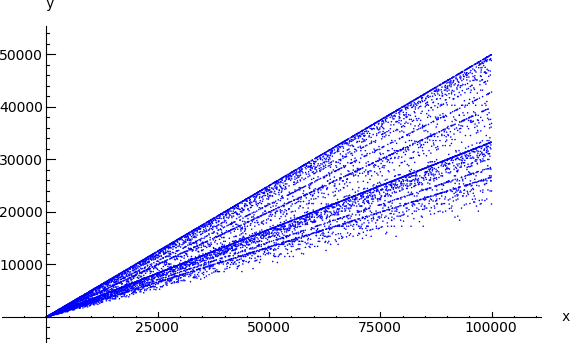
\includegraphics{figures/primitive-roots-all}
\caption{The number of primitive roots of all primes between 1 and 100,000.}
\label{fig:primitive_roots_all}
\end{figure}

\vskip +50 pt
Figure~\ref{fig:primitive_roots_smallest} graphs the smallest
primitive roots of all primes between 1 and 100,000. The $x$-axis
represents primes between 1 and 100,000. The $y$-axis represents the
smallest primitive root of each prime within that
interval.

\vskip +25 pt
Figure~\ref{fig:primitive_roots_largest} shows a
corresponding graph for the largest primitive root of each prime
within the above interval.

\begin{figure}[!htbp]
\centering
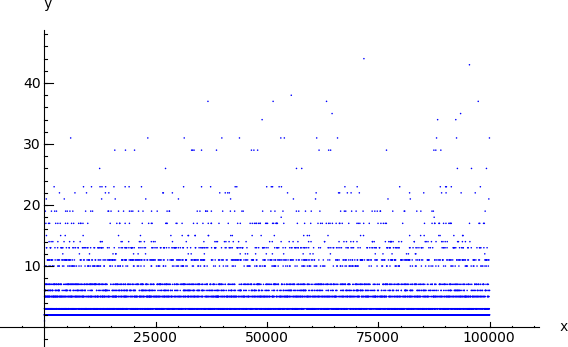
\includegraphics{figures/primitive-roots-smallest}
\caption{The smallest primitive roots of all primes between 1 and 100,000.}
\label{fig:primitive_roots_smallest}
\end{figure}

\begin{figure}[!htbp]
\centering
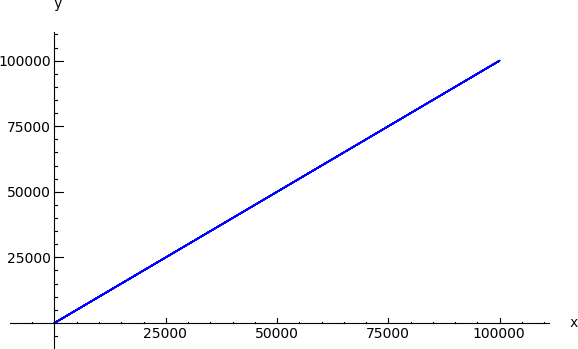
\includegraphics{figures/primitive-roots-largest}
\caption{The largest primitive roots of all primes between 1 and 100,000.}
\label{fig:primitive_roots_largest}
\end{figure}

% To enforce that the next chapter starts at the beginning of a new page after
% the freely placed graphics, it is necessary to have TWO newpages and in between
% something to be printed (here invisible blanks).
% \newpage
% $ $



% ---------------------------------------------------------------------------
\newpage
\hypertarget{NumberTheory_Sage_RSA sample}{}
\subsection{RSA examples with Sage}
\label{l:NumberTheory_Sage_RSA sample}{}

\noindent Below is Sage source code for the simple RSA examples in
section~\ref{rsaconcrete} (``\nameref{rsaconcrete}''). 

\vskip +10 pt 
\hypertarget{AppArith4a}{%
\noindent \textbf{Example on page~\pageref{SrcArith4a}:}} \\
The RSA exponentiation $M^{37} \pmod{3713}$ on message $M = 120$ can be
calculated in Sage as follows:

\begin{Verbatim}%
[fontsize=\footnotesize,fontshape=tt]
sage: power_mod(120, 37, 3713)
1404
\end{Verbatim}


\vskip +10 pt 
\hypertarget{AppArith4b}{%
\noindent {\bf Example on page~\pageref{SrcArith4b}:}} \\
The factorization of $J(256027) = 255016 = 2^3 * 127 * 251$ can be
calculated using Sage as follows:

\begin{sagecode}
\begin{Verbatim}%
[fontsize=\footnotesize,fontshape=tt]
sage: factor(255016)
2^3 * 127 * 251
\end{Verbatim}
\caption{Factoring a number}
\end{sagecode}


\vskip +10 pt 
\hypertarget{AppArith4c}{%
\noindent {\bf Example on page~\pageref{SrcArith4c}:}} \\
Sage can do RSA encryption as follows:

\begin{sagecode}
\begin{Verbatim}%
[fontsize=\footnotesize,fontshape=tt]
sage: A = [82, 83, 65, 32, 119, 111, 114, 107, 115, 33]
sage: e = 65537; m = 256027
sage: [power_mod(a, e, m) for a in A]
[212984, 25546, 104529, 31692, 248407, 100412, 54196, 100184, 58179, 227433]
\end{Verbatim}
\caption{RSA encryption by modular exponentiation of a number (used as message)}
\end{sagecode}


\vskip +10 pt 
\hypertarget{AppArith4d}{%
\noindent {\bf Example on page~\pageref{SrcArith4d}:}} \\
RSA encryption using Sage:

\begin{Verbatim}%
[fontsize=\footnotesize,fontshape=tt]
sage: A = [21075, 16672, 30575, 29291, 29473]
sage: e = 65537; m = 256027
sage: [power_mod(a, e, m) for a in A]
[158721, 137346, 37358, 240130, 112898]
\end{Verbatim}


\vskip +10 pt 
\hypertarget{AppArith4e}{%
\noindent {\bf Example on page~\pageref{SrcArith4e}:}} \\
RSA encryption using Sage:

\begin{Verbatim}%
[fontsize=\footnotesize,fontshape=tt]
sage: A = [82083, 65032, 119111, 114107, 115033]
sage: e = 65537; m = 256027
sage: [power_mod(a, e, m) for a in A]
[198967, 51405, 254571, 115318, 14251]
\end{Verbatim}





% ++++++++++++++++++++++++++++++++++++++++++++++++++++++++++++++++++++++++++
% \vskip +12pt
\newpage
\hypertarget{NumberTheory_Appendix_F}{}  %\hypertarget{AppendixListAndDef}{}
\section{Appendix: List of the definitions and theorems formulated in this chapter}
\label{l:NumberTheory_Appendix_F}{}  %\label{l:AppendixListAndDef}{}

% \vskip +8 pt
\begin{center}
\begin{tabular}{|l|l|l|}\hline
 & Short description ~~ & Page \\ \hline
Definition~\ref{def-zth-prime} & prime numbers &  \pageref{def-zth-prime} \\
Definition~\ref{def-zth-composite} & composite numbers & \pageref{def-zth-composite}  \\ \hline
Theorem~\ref{thm-zth-cnum} & factors of composite numbers~~~~~~~ & \pageref{thm-zth-cnum}\\
Theorem~\ref{thm-zth-mthm} &  1st fundamental theorem of number theory &  \pageref{thm-zth-mthm} \\  \hline
Definition~\ref{def-zth-divisibility} & divisibility & \pageref{def-zth-divisibility} \\
Definition~\ref{def-zth-remainder} & remainder class $r$ modulo $m$ & \pageref{def-zth-remainder} \\
Definition~\ref{def-zth-congruence} & congruent & \pageref{def-zth-congruence} \\ \hline
Theorem~\ref{thm-zth-div} & congruence with difference  & \pageref{thm-zth-div} \\
Theorem~\ref{thm-zth-multinv} & multiplicative inverse (existance) & \pageref{thm-zth-multinv}  \\
Theorem~\ref{thm-zth-exhperm} & exhaustive permutation & \pageref{thm-zth-exhperm} \\
Theorem~\ref{thm-zth-pot} & power mod $m$ & \pageref{thm-zth-pot} \\ \hline
Definition~\ref{def-zth-zn} & $\mathbb{Z}_n$  & \pageref{def-zth-zn}\\
Definition~\ref{def-zth-znmult} &   $\mathbb{Z}_n^*$ & \pageref{def-zth-znmult} \\ \hline
Theorem~\ref{thm-zth-znmult} & multiplicative inverse in $\mathbb{Z}_n^*$& \pageref{thm-zth-znmult} \\ \hline
Definition~\ref{def-zth-phiofn} & Euler function $J(n)$ & \pageref{def-zth-phiofn} \\
Theorem~\ref{thm-zth-phiprime} & $J(p)$ &  \pageref{thm-zth-phiprime}\\
Theorem~\ref{thm-zth-phipq} & $J(p*q)$ &  \pageref{thm-zth-phipq}\\
Theorem~\ref{thm-zth-phimultprime} & $J(p_1 * \cdots *p_k)$ & \pageref{thm-zth-phimultprime} \\
Theorem~\ref{thm-zth-phinum} & $J(p_1^{e_1} * \cdots *p_k^{e_k})$ & \pageref{thm-zth-phinum} \\
Theorem~\ref{thm-zth-fermat1} & little Fermat  &  \pageref{thm-zth-fermat1}\\
Theorem~\ref{thm-zth-fermateuler} & Euler-Fermat theorem & \pageref{thm-zth-fermateuler} \\ \hline
Definition~\ref{def-zth-ordn} & multiplicative order $ {\rm ord}_{m} (a)$ & \pageref{def-zth-ordn} \\
Definition~\ref{def-zth-primitiveroot} & primitive root of $m$ &  \pageref{def-zth-primitiveroot}\\
Theorem~\ref{thm-zth-ordp} & exhausting of all possible values & \pageref{thm-zth-ordp} \\ \hline
\end{tabular}
\end{center}
\vskip +6 pt





% ++++++++++++++++++++++++++++++++++++++++++++++++++++++++++++++++++++++++++
% ++++++++++++++++++++++++++++++++++++++++++++++++++++++++++++++++++++++++++
\newpage
\begin{thebibliography}{99999}
\addcontentsline{toc}{section}{Bibliography}

\bibitem[Agrawal2002]{nt:Agrawal2002}  \index{Agrawal 2002} 
    M. Agrawal, N. Kayal, N. Saxena, \\
    {\em PRIMES in P}, August 2002, revised paper: \\
       \href{http://www.cse.iitk.ac.in/~manindra/algebra/primality_v6.pdf}
    {\texttt{http://www.cse.iitk.ac.in/~manindra/algebra/primality\_v6.pdf}} \\
    See also the website "The AKS "PRIMES in P" Algorithm Resource":
       \href{http://fatphil.org/maths/AKS/}
    {\texttt{http://fatphil.org/maths/AKS/}}

\bibitem[Bartholome1996]{nt:3Bartholome1996}  \index{Bartholome 1996} 
    A. Bartholome, J. Rung, H. Kern, \\
    {\em Zahlentheorie f\"ur Einsteiger}, Vieweg 1995, 2nd edition 1996.

\bibitem[Bauer1995]{nt:Bauer1995} \index{Bauer 1995}
    Friedrich L. Bauer, \\
    {\em Entzifferte Geheimnisse}, Springer, 1995.

\bibitem[Bauer2000]{nt:Bauer2000} \index{Bauer 2000}
    Friedrich L. Bauer, \\
    {\em Decrypted Secrets}, Springer 1997, 2nd edition 2000.

\bibitem[Bernstein2001]{nt:Bernstein2001} \index{Bernstein 2001}
    D.~J. Bernstein, \\
    {\em Circuits for integer factorization: a proposal},\\ 
    \href{http://cr.yp.to/papers/nfscircuit.ps}
    {\texttt{http://cr.yp.to/papers/nfscircuit.ps}} \\
    \href{http://cr.yp.to/djb.html}{\texttt{http://cr.yp.to/djb.html}}

\bibitem[Beutelspacher1996]{nt:Beutelspacher1996} \index{Beutelspacher 1996}
    Albrecht Beutelspacher, \\
    {\em Kryptologie}, Vieweg 1987, 5th edition 1996.

\bibitem[Bourseau2002]{nt:Bourseau2002} \index{Bourseau 2002} \index{Fox 2002}
    F. Bourseau, D. Fox, C. Thiel, \\
    {\em Vorz\"uge und Grenzen des RSA-Verfahrens},\\
    In: Datenschutz und Datensicherheit (DuD) 26/2002, pp~84-89 (see www.dud.de),
    \href{http://http://www.secorvo.de/publikationen/rsa-grenzen-fox-2002.pdf}
         {\texttt{http://www.secorvo.de/publikationen/rsa-grenzen-fox-2002.pdf}}

\bibitem[Brands2002]{nt:Brands2002} \index{Brands 2002}
    Gilbert Brands, \\
    {\em Verschl\"usselungsalgorithmen -- Angewandte Zahlentheorie 
    rund um Sicherheitsprotokolle}, Vieweg, 2002.

\bibitem[Buchmann2004]{nt:Buchmann2004} \index{Buchmann 2004}
    Johannes Buchmann, \\
    {\em Introduction to Cryptography}, Springer, 2nd edition, 2004.

\bibitem[Buhler1993]{nt:Buhler1993} \index{Buhler 1993} 
    J.P. Buhler, H.W. Lenstra, C. Pomerance, \\
    {\em Factoring integers with the number field sieve}, \\
    In: A.K. Lenstra, H.W. Lenstra (Hrsg.): The Development of the 
    Number Field Sieve, Lecture Notes in Mathematics, Vol.~1554, 
    Springer, Heidelberg 1993, pp~50$-$94.

\bibitem[Eckert2003]{nt:Eckert2003} \index{Eckert 2003}
    Claudia Eckert, \\
    {\em IT-Sicherheit: Konzepte-Verfahren-Protokolle}, 
    Oldenbourg 2001, 2nd edition 2003.

\bibitem[Ertel2001]{nt:Ertel2001} \index{Ertel 2001} 
    Wolfgang Ertel, \\
    {\em Angewandte Kryptographie}, 
    Fachbuchverlag Leipzig FV 2001.

\bibitem[GISA2002]{nt:GISA2002} \index{GISA 2002}
    GISA (German Information Security Agency), \\
    {\em Recommendation for key length selection}, Bonn, Sep. 2002, \\
    \href{http://www.bsi.bund.de/esig/basics/techbas/krypto/bund02v7.pdf}
    {\tt http://www.bsi.bund.de/esig/basics/techbas/krypto/bund02v7.pdf} \\
    A statement on these recommendations: \\
    \href{http://www.secorvo.de/publikat/stellungnahme-algorithmenempfehlung-020307.pdf}
    {\texttt{http://www.secorvo.de/publikat/}}\\
    \hspace*{1cm}
    \href{http://www.secorvo.de/publikat/stellungnahme-algorithmenempfehlung-020307.pdf}
    {\texttt{stellungnahme-algorithmenempfehlung-020307.pdf}}

\bibitem[Graham1994]{nt:Graham1994} \index{Graham 1994}
    Graham, Knuth, Patashnik, \\
    {\em Concrete Mathemathics, a Foundation of Computer Science}, \\
    Addison Wesley 1989, 6th printing 1994.

\bibitem[Kippenhahn1997]{nt:Kippenhahn1997} \index{Kippenhahn 1997}
    Rudolph Kippenhahn, \\
    {\em Verschl\"usselte Botschaften -- Geheimschrift, Enigma und Chipkarte}, 
    Rowohlt, 1997.

\bibitem[Kippenhahn1999]{nt:Kippenhahn1999} \index{Kippenhahn 1999}
    Rudolph Kippenhahn, \\
    {\em Code Breaking -- A History and Exploration}, 
    Constable, 1999.

\bibitem[Knuth1998]{nt:Knuth1998} \index{Knuth 1998}
    Donald E. Knuth, \\
    {\em The Art of Computer Programming, vol 2: Seminumerical Algorithms}, \\
    Addison-Wesley, 2nd edition 1998.
    % wann war erste Edition ?

\bibitem[Lenstra1993]{nt:Lenstra1993} \index{Lenstra 1993}
     A. Lenstra, H. Lenstra: \\ 
     {\em The development of the Number Field Sieve}, \\
     Lecture Notes in Mathematics 1554, Springer, New York 1993

\bibitem[Lenstra1999]{nt:Lenstra1999} Arjen K. Lenstra, Eric R. Verheul
     \index{Lenstra/Verheul 1999} \\
     {\em Selecting Cryptographic Key Sizes (1999)},\\
     Journal of Cryptology: the journal of the International 
     Association for Cryptologic Research \\
     \href{http://www.cryptosavvy.com/cryptosizes.pdf}
     {\texttt{http://www.cryptosavvy.com/cryptosizes.pdf}}

\bibitem[Lenstra2002]{nt:Lenstra2002} \index{Lenstra 2002}
    Arjen K. Lenstra, Adi Shamir, Jim Tomlinson, Eran Tromer,\\
    {\em Analysis of Bernstein's Factorization Circuit},\\
    \href{http://www.cryptosavvy.com/mesh.pdf}
    {\texttt{http://www.cryptosavvy.com/mesh.pdf}}

\bibitem[Menezes2001]{nt:Menezes2001} \index{Menezes 2001}
    Alfred J. Menezes, Paul C. van Oorschot, Scott A. Vanstone \\
    {\em Handbook of Applied Cryptography}, 
    CRC Press 1997, 5th printing 2001.

\bibitem[Pfleeger1997]{nt:Pfleeger1997} \index{Pfleeger 1997}
    Charles P. Pfleeger, \\
    {\em Security in Computing}, Prentice-Hall, 2nd edition 1997.
    % im Buch stand nicht, wann die 1. Edition rauskam.

\bibitem[Pomerance1984]{nt:Pomerance1984} \index{Pomerance 1984} 
    C. Pomerance, \\
    {\em The quadratic sieve factoring algorithm}, \\
    In: G.R. Blakley, D. Chaum (Hrsg.): Proceedings of Crypto '84, 
    LNCS 196, Springer Berlin 1995, pp~169-182.

\bibitem[RSA Security 2002]{nt:RSA Security 2002} \index{RSA Security 2002} 
    RSA Security, \\
    {\em Has the RSA algorithm been compromised as a result 
    of Bernstein's Paper?}, \\
    April 8th, 2002, \\
    \href{http://www.rsasecurity.com/}{\tt http://www.rsasecurity.com/}
    
\bibitem[SchneiderM2004]{nt:SchneiderM2004} \index{SchneiderM 2004} 
    Matthias Schneider, \\
    {\em Analyse der Sicherheit des RSA-Algorithmus. \\
     M\"ogliche Angriffe, deren Einfluss auf sichere Implementierungen und \"okonomische Konsequenzen}, \\
    Diploma thesis at the University of Siegen, Germany, 2004.

\bibitem[Schneier1996]{nt:Schneier1996nt} \index{Schneier 1996} 
    Bruce Schneier, \\
    {\em Applied Cryptography, Protocols, Algorithms, and Source Code in C}, \\
    Wiley and Sons, 2nd edition 1996.

\bibitem[Schwenk2002]{nt:Schwenk2002}\index{Schwenk 2002}
    J\"org Schwenk, \\
    {\em Sicherheit und Kryptographie im Internet}, 
    Vieweg 2002.

\bibitem[Sedgewick1990]{nt:Sedgewick1990} \index{Sedgewick 1990}
    Robert Sedgewick,\\
    {\em Algorithms in C}, Addison-Wesley, 1990.

\bibitem[Shamir2003]{nt:Shamir2003} \index{Shamir 2003} \index{TWIRL device} 
    Adi Shamir, Eran Tromer, \\
    {\em Factoring Large Numbers with the TWIRL Device}, 
    Januar 2003, \\
    \href{http://www.wisdom.weizmann.ac.il/~tromer/}
    {\texttt{http://www.wisdom.weizmann.ac.il/\~{}tromer/}}.

\bibitem[Shamir2003a]{nt:Shamir2003a} \index{Shamir 2003a} \index{TWIRL device} 
    Adi Shamir, Eran Tromer, \\
    {\em On the Cost of Factoring RSA-1024}, 
    RSA Laboratories CryptoBytes Volume 6, No. 2, Summer 2003, p. 11-20 \\
    \url{http://www.rsasecurity.com/rsalabs/cryptobytes/CryptoBytes_August_2003.pdf}

\bibitem[Silverman2000]{nt:Silverman2000} \index{Silverman 2000}
     Robert D. Silverman: \\ 
     {\em A Cost-Based Security Analysis of Symmetric and Asymmetric 
          Key Lengths} \\
     In: RSA Laboratories Bulletin, No. 13, April 2000, p. 1-22

\bibitem[Stinson1995]{nt:Stinson1995} \index{Stinson 1995}
    Douglas R. Stinson,\\
    {\em Cryptography - Theory and Practice}, CRC Press, 1995.

\bibitem[Weis2003]{nt:Weis2003} \index{Weis 2003} \index{Lucks 2003} \index{Bogk 2003}
    R\"udiger Weis, Stefan Lucks, Andreas Bogk, \\
    {\em Sicherheit von 1024 bit RSA-Schl\"usseln gef\"ahrdet},\\
    In: Datenschutz und Datensicherheit (DuD) 6/2003, pp~360-362 (see www.dud.de)\\
    The article explains details about the TWIRL device\index{TWIRL device}.

\bibitem[Welschenbach2001]{nt:Welschenbach2001} \index{Welschenbach 2001}
    Welschenbach, Michael, \\
    {\em Kryptographie in C und C++}, Springer 2001.
    
\bibitem[Wiles1994]{nt:Wiles1994} \index{Wiles, Andrew}
    Wiles, Andrew, \\
    {\em Modular elliptic curves and Fermat's Last Theorem}, 
    \index{Fermat!last theorem} \\
    In: Annals of Mathematics 141 (1995).

\bibitem[Wolfenstetter1998]{nt:Wolfenstetter1998} \index{Wolfenstetter 1998}
    Albrecht Beutelspacher, J\"org Schwenk, Klaus-Dieter Wolfenstetter, \\
    {\em Moderne Verfahren in der Kryptographie}, 
    Vieweg 1995, 2nd edition 1998.

\bibitem[Yan2000]{nt:Yan2000} \index{Yan 2000} 
    Song Y. Yan, \\
    {\em Number Theory for Computing}, Springer, 2000.
\end{thebibliography}



% ++++++++++++++++++++++++++++++++++++++++++++++++++++++++++++++++++++++++++
\newpage
\section*{Web links}
\addcontentsline{toc}{section}{Web links}

\begin{enumerate}
   \item \hypertarget{knott}{}  \index{Knott, Ron}
         Ron Knott's Fibonacci \index{Fibonacci} page, \\
         Here, everything revolves around Fibonacci numbers.\\
         \href{http://www.mcs.surrey.ac.uk/personal/R.Knott/Fibonacci/fib.html}
         {\texttt{http://www.mcs.surrey.ac.uk/personal/R.Knott/Fibonacci/fib.html}}
          
   \item CrypTool, \index{CrypTool} \\
         Open source e-learning software to illustrate cryptography and cryptanalysis\\
         \href{http://www.cryptool.de}{\texttt{http://www.cryptool.de}},\\
         \href{http://www.cryptool.org}{\texttt{http://www.cryptool.org}},\\ 
         \href{http://www.cryptool.com}{\texttt{http://www.cryptool.com}}
          
   \item Mathematica, \index{Mathematica} \\
         Commercial mathematics package \\
         \href{http://www.wolfram.com}{\texttt{http://www.wolfram.com }}
          
   \item LiDIA, \index{LiDIA} \\
         Extensive library containing number-theory functions and the LC interpreter \\
         \href{http://www.informatik.tu-darmstadt.de/TI/LiDIA}
         {\texttt{http://www.informatik.tu-darmstadt.de/TI/LiDIA}}
          
   \item BC, \index{BC} \\
         Interpreter with number-theory functions \\
         \href{http://www.gnu.org/software/bc/bc.html}
         {\texttt{http://www.gnu.org/software/bc/bc.html}}
          
   \item Pari-GP, \index{Pari-GP} \\
         Excellent, fast, free interpreter with number theoretical functions.\\
         \href{http://pari.math.u-bordeaux.fr/}
              {\texttt{http://pari.math.u-bordeaux.fr/}}\\
         \href{http://en.wikipedia.org/wiki/PARI/GP}
              {\texttt{http://en.wikipedia.org/wiki/PARI/GP}}\\
         Resources for PARI/GP at Karim Belabas's website:\\
         \href{http://www.math.u-bordeaux.fr/~belabas/pari/}
              {\texttt{http://www.math.u-bordeaux.fr/\~{}belabas/pari/}}
           
   \item \index{Munchenbach@M\"unchenbach, Carsten}
         Only after I had completed this article, did I come across the
         website of Mr.\ M\"unchenbach, which interactively and didactically
         uses elementary number theory to provide a sophisticated
         description of the fundamental mathematical thought processes. 
         It was created for a teaching project in the 11th grade 
         of the technical grammar school (unfortunately only available in German): \\
         \href{http://www.hydrargyrum.de/kryptographie}
         {\texttt{http://www.hydrargyrum.de/kryptographie}}
                      
   \item Web site of Mr.~Wagner, who is responsible for the development
	 of the curriculum of computer science in one of the German federal 
         states (L\"ander). Here you can get hold of a collection of texts
	 and (Java-)\discretionary{}{}{}programs (available only in German):\\
         \href{http://www.saar.de/~awa/kryptolo.htm}
         {\texttt{http://www.saar.de/\~{}awa/kryptolo.htm}}
          
   \item GISA, \index{GISA} \\
         German Information Security Agency \\
         \href{http://www.bsi.bund.de}{\texttt{http://www.bsi.bund.de}}

   \item Factorization records and challenges\index{Factorization!factoring records},\\
         \href{http://www.crypto-world.com/}
           {\texttt{http://www.crypto-world.com/}} \\
         \href{http://www.crypto-world.com/FactorWorld.html}
           {\texttt{http://www.crypto-world.com/FactorWorld.html}}, page by Scott Contini \\
         \href{http://www.loria.fr/~zimmerma/records/factor.html}
           {\texttt{http://www.loria.fr/\~{}zimmerma/records/factor.html}} \\
         \href{http://www.tutorgig.com/ed/RSA\_number}
           {\texttt{http://www.tutorgig.com/ed/RSA\_number}} \\

         \href{http://www.uni-bonn.de/Aktuelles/Pressemitteilungen/pm02/pm035-02.html}
           {\texttt{http://www.uni-bonn.de/Aktuelles/Pressemitteilungen/pm02/pm035-02.html}} \\
         \href{http://www.ercim.org/publication/Ercim\_News/enw49/franke.html, 2002-01}
           {\texttt{http://www.ercim.org/publication/Ercim\_News/enw49/franke.html, 2002-01}} \\
         \href{http://www.loria.fr/~zimmerma/records/rsa160}
           {\texttt{http://www.loria.fr/\~{}zimmerma/records/rsa160}} \\
 
         \href{http://www.rsa.com/rsalabs/node.asp?id=2092}
           {\texttt{http://www.rsa.com/rsalabs/node.asp?id=2092}}\\
	 
   \item The Cunningham Project, \index{Cunningham project}\\ 
         \href{http://www.cerias.purdue.edu/homes/ssw/cun/}
         {\texttt{http://www.cerias.purdue.edu/homes/ssw/cun/}}

   \item Sage, \index{Sage} \\
         Excellent, open source computer algebra system with Python as script language,
	 used to build the code samples in this chapter.
	 See the introduction in chapter~\ref{s:appendix-using-sage}.\\
         \href{http://www.sagemath.org/}
              {\texttt{http://www.sagemath.org/}}\\
         \href{http://en.wikipedia.org/wiki/Sage_%28mathematics_software%29}
              {\texttt{http://en.wikipedia.org/wiki/Sage\_\%28mathematics\_software\%29}}\\

\end{enumerate}



% ++++++++++++++++++++++++++++++++++++++++++++++++++++++++++++++++++++++++++
\vskip +20 pt
\section*{Acknowledgments}
\addcontentsline{toc}{section}{Acknowledgments}

I would like to take this opportunity to thank 
\begin{itemize}

  \item {Henrik Koy for making many very useful suggestions, 
         for the very constructive proof-reading of the first version of
	 this article, and for helping with TeX. \\
	 Mr.\ Koy designed and developed in his leisure time the 
	 functions and the complex dialog box of the RSA cryptosystem within CrypTool, 
	 which enables you to execute the RSA samples of this article.}

  \item {J\"org Cornelius Schneider for his enthusiastic TeX support and for the
         many cases where he helped when facing programming or design problems.}
  
  \item {Dr.\ Georg Illies for pointing me to Pari-GP\index{Pari-GP}.}
  
  \item {Lars Fischer for his help with fast Pari-GP\index{Pari-GP} code for primitive roots.}
  
  \item {Minh Van Nguyen from Australia for his always fast, professional and exhaustive
         help with the Sage\index{Sage} code samples in this chapter.}

\end{itemize}



% Local Variables:
% TeX-master: "../script-en.tex"
% End:
